\documentclass{textbook}

\begin{document}

  \frontmatter

  % Title page
  \pdfbookmark[section]{Title}{title}
  \newgeometry{margin=2.5in}
  \thispagestyle{empty}
  \ThisLRCornerWallPaper{1}{cover}
  \begin{center}
    {\huge\bfseries An Introduction to}
    \vspace{1em}\par
    {\Huge\bfseries Machine Learning}
    \vspace{0.25in}\par
    {\large A textbook for Harvard's CS181}
    \vfill
  \end{center}
  \clearpage

  % Acknowledgment
  % \pdfbookmark[section]{Acknowledgment}{acknowledgment}
  \newgeometry{margin=2.5in}
  \thispagestyle{empty}
  \begin{center}
    {\small Thank you to William J. Deuschle, the original author of this textbook, and to course staffs and students for maintaining this work across the years.}
    \vfill
    {\small Last updated February 2022.}
  \end{center}
  \clearpage

  % Epigraph
  \vspace*{2in}
  \thispagestyle{empty}
  {\itshape ``Nobody phrases it this way, but I think that artificial intelligence is almost a humanities discipline. It’s really an attempt to understand human intelligence and human cognition.''}
  \vskip 0.1in
  {\hfill - Sebastian Thrun}
  \clearpage
  \restoregeometry

  % Table of contents
  \pdfbookmark[section]{Contents}{toc}
	\tableofcontents
  \clearpage

  % Notation
  \markboth{NOTATION}{}
  \chapter*{Notation}
\addcontentsline{toc}{chapter}{\protect\numberline{}Notation}%

The machine learning community is notorious for using widly varying notations. The following standard is not meant to provide a standard lookup for all machine learning literature, but specifically for this textbook. The fastest way to become fluent in understanding notation is by reading machine learning papers.
% Breakdown of notation is standard in ML and is shared with D2l.ai and Machine Learning book.

% \verb|https://nthu-datalab.github.io/ml/slides/Notation.pdf|

% \verb|https://d2l.ai/chapter_notation/index.html|

\renewcommand{\arraystretch}{1.15}
\subsection*{Set theory}
\begin{tabular}{p{0.13\linewidth}p{0.07\linewidth}p{0.80\linewidth}}
  $\mathcal{A}$             &   & a set \\
  $\mathbb{N}$              &   & the set of all natural numbers \\
  $\mathbb{N}^*$            &   & the set of all natural numbers excluding 0 \\
  $\mathbb{Z}$              &   & the set of all integers \\
  $\mathbb{R}$              &   & the set of all real numbers \\
  $\mathbb{R}^D$            &   & the set of all real-valued $D$-dimensional vectors \\
  $\mathbb{R}^{N \times D}$ &   & the set of all real-valued $N \times D$ matrices \\
\end{tabular}


\subsection*{Numerical objects}
% \begin{tabular}{p{0.13\linewidth}p{0.07\linewidth}p{0.80\linewidth}}
%   $x$            & $\mathbb{R}$              & a scalar \\
%   $\mathbf{x}$   & $\mathbb{R}^D$            & a vector \\
%   $\mathbf{X}$   & $\mathbb{R}^{N \times D}$ & a matrix \\
%   %  $\mathsf{X}$ & $\mathbb{R}$ & a general tensor \\
%   $\mathbf{I}_N$ & $\mathbb{R}^{N \times N}$ & the identify matrix \\
% \end{tabular}
\begin{tabular}{p{0.2\linewidth}p{0.8\linewidth}}
  $x \in \mathbb R$ & a scalar \\
  $\bm x \in \mathbb R^D$ & a vector \\
  $\bm X \in \mathbb{R}^{N \times D}$ & a matrix \\
  %  $\mathsf{X}$ & $\mathbb{R}$ & a general tensor \\
  $\bm I_N \in \mathbb{R}^{N \times N}$ & the identify matrix \\
\end{tabular}


\subsection*{Functions and operators}
\begin{tabular}{p{0.23\linewidth}p{0.75\linewidth}}
  $a := b$ or $b =: a$ &  $a$ is defined to be $b$ \\
  $f : \mathcal{A} \to \mathcal{B}$ &  a function $f$ that maps from domain $\mathcal{A}$ to codomain $\mathcal{B}$ \\
  $f \circ g $ & the composite function $f(g(\cdot))$ \\
  $f(x;\, \theta)$ & a function of $x$ parametrized by $\theta$ \\
  $\log(\cdot)$ & the natural logarithm \\
  $\log_b(\cdot)$ & the base $b$ logarithm \\
  $||\mathbf{x}||_p$ & the $L^p$ norm of $\mathbf{x}$ \\
  $||\mathbf{x}||$ & the $L^2$ norm of $\mathbf{x}$ \\
  $\bm{1}(\cdot)$ & the indicator function, evaluates to 1 if argument is true else 0 \\
\end{tabular}


\subsection*{Probability theory}
\begin{tabular}{p{0.13\linewidth}p{0.07\linewidth}p{0.80\linewidth}}
  $\mathrm x$           & $\mathbb{R}$   & a scalar-valued r.v. \\
  $\mathbf x$      & $\mathbb{R}^D$ & a vector-valued r.v. \\
  $\mathbf X$      & $\mathbb{R}^{N\times D}$ & a matrix-valued r.v. \\
  % $X \perp Y$   &                & r.v.s $X$ and $Y$ are independent \\
  % $X \perp Y \mid Z$   &            & r.v.s $X$ and $Y$ are conditionally independent given $Z$\\
  $\mathrm x \sim \operatorname{P}$    &                & r.v. $X$ is distributed as some distribution $\operatorname{P}$ \\
  $\mathrm x \sim p(x)$ &                & r.v. $X$ is distributed as some distribution whose PDF is $p(x)$ \\
  $P(\mathrm x = x)$    &                & the probability of the event $X$ takes on value $x$ \\
  $\E[X]$       &                & expectation of r.v. $X$ \\
  $\Var(X)$  &                & variance of r.v $X$ \\
  $\Cov(X, Y)$  &                & covariance of r.v.s $X$ and $Y$ \\
  $\mathcal{N}(\mu, \sigma)$ & & the Guassian distribution with mean $\bm\mu$ and covariance matrix $\bm\Sigma$ \\
  $\mathcal{N}(x;\, \mu, \sigma)$ & & the PDF of the distribution $\mathcal{N}(\mu, \Sigma)$ \\
\end{tabular}


\subsection*{Indexing}
\begin{tabular}{p{0.13\linewidth}p{0.07\linewidth}p{0.80\linewidth}}
  $x_i$,  $[\mathbf{x}]_i$         & $\mathbb{R}$   & the $i$-th element of vector $\mathbf{x}$ \\
  $x_{i,j}$, $[\mathbf{X}]_{i,j}$ & $\mathbb{R}$   & the element of matrix $\mathbf{X}$ at row $i$ and column $j$. Commas in the subscript can be ommitted if not ambiguous. \\
  $\mathbf{X}_{:,j}$              & $\mathbb{R}^N$ & the $j$-th column of matrix $\mathbf{X} \in \mathbb{R}^{N \times D}$  \\
  $\mathbf{X}_{i,:}$              & $\mathbb{R}^D$ & the $i$-th row of matrix $\mathbf{X} \in \mathbb{R}^{N \times D}$  \\
\end{tabular}

\subsection*{Object generation}
\begin{tabular}{p{0.13\linewidth}p{0.07\linewidth}p{0.80\linewidth}}
  $[a:b]$                                &                           & the set of integers $\mathbb Z \cup [a, b]$ between $a$ and $b$ (inclusive) \\
  $[a]$                                  &                           & the set of integers $[1:a]$ \\
  $\{x_i\}_{n=1}^{N}$                    &                           & the set of $N$ objects $x_1, \dots, x_N$. \\
  $[\bm{x}_1, \ldots, \bm{x}_n]$ & $\mathbb{R}^{d \times n}$ & the matrix $\bm{X}$ such that $\bm{X}_{:,i} = x_i$ where $x_i \in \mathbb{R}^d$ \\
\end{tabular}

\subsection*{Machine learning}
\begin{tabular}{p{0.13\linewidth}p{0.07\linewidth}p{0.80\linewidth}}
  $N$ & $\mathbb R$ & number of datapoints in our training dataset \\
  $D$ & $\mathbb R$ & number of features in each datapoint; dimensionality of our input space \\
  $x$ & $\mathcal X$ & An example. Here, $\mathcal X$ is our input space. Usually, $\mathcal X = \mathbb R^D$. \\
  $x^*$ & $\mathcal X$ & A test example. This is refers to an example outside our training dataset whose label we do not know and are trying to predict. \\
  $y$ & $\mathcal Y$ & A label. Here, $\mathcal Y$ is our output space. In linear regression, $\mathcal Y = \mathbb R$. \\
  $\hat y^*$ &  $\mathcal Y$ & A predicted label. This is the label our model predicts for some test example $x^*$. \\
  $w$ or $\theta$ & $\mathcal W$ & The model weights \\
  $\mathcal L : \mathcal W \to \mathbb R$ & & a loss or objective function \\
  \mbox{$f : \mathcal X \times \mathcal W \to \mathcal Y$} & & a model parametrized by possible weights $\mathcal W$. \\
\end{tabular}

% \subsection*{Abbreviations}
% \begin{tabular}{p{0.23\linewidth}p{0.75\linewidth}}
%   r.v. & random variable
%   % GMM & Gaussian mixture model
% \end{tabular}

  \clearpage

  % Textbook chapters
  \mainmatter
  \chapter{Introduction}

Machine learning refers to the study of algorithms which improve automatically through experience or the use of data. These algorithms often build some model, or mathematical understanding of the world, based on data which we, the humans, provide. After learning from this data, a model can help us make predictions, decision, or conclusions that we never explicitly programmed or even knew beforehand. A bank, for example, may use some machine learning algorithm to inform their decisions on who they should give out loans to. With this algorithm, the bank hopes to achieve its original goal of making fewer risky investments.

Indeed, machine learning is indeed very useful in aiding human decision making. However, it is irresponsible of us to surrender all our decision-power onto machines. If the bank's machine learning algorithm learned from historical data, it may learn to distrust certain demographics who have been socio-economically disadvantaged in the past, thus perpetuating historical prejudices by refusing to recommend loans to the people of these communities. Machine learning has made it all too easy to simply delegate our actions onto whatever an algorithm tells us will ``maximize profits'' or ``minimize cost''. Too often are these algorithms are built thoughtlessly and used within some decision-system wrecklessly. The purpose of this book is to provide a framework with which to approach machine learning problems and understand how these tools we create ought to be situated in the real world.

\section{Data representation}

\begin{figure}
    \centering
    \begin{subfigure}{0.49\textwidth}
        \centering
        \begin{tabular}{llll}\toprule
        Name   & Age  & Weight  & Height \\ \midrule
        Juan   & $18$ & $162$lb & $6$ft $1$in \\
        Joe    & $34$ & $146$lb & $5$ft $10$in \\
        Mei    & $39$ & $193$lb & $5$ft $8$in \\
        Bella  & $21$ & $124$lb & $5$ft $3$in \\
        Abdul  & $57$ & $141$lb & $5$ft $7$in \\
        Hanna  & $40$ & $134$lb & $5$ft $4$in \\ \bottomrule
        \end{tabular}
        \caption{Data in raw representation.}
        \label{fig:data represented by vectors a}
    \end{subfigure}
    \begin{subfigure}{0.5\textwidth}
        \centering
        \begin{tabular}{llll}\toprule
        Age  & Weight (kg) & Height (cm) \\ \midrule
        $18$ & $73.48$ & $185.42$ \\
        $34$ & $66.22$ & $177.80$ \\
        $39$ & $87.54$ & $172.72$ \\
        $21$ & $56.25$ & $160.02$ \\
        $57$ & $63.96$ & $170.18$ \\
        $40$ & $60.78$ & $162.56$ \\ \bottomrule
        \end{tabular}
        \caption{Data in numerical representation.}
        \label{fig:data represented by vectors b}
    \end{subfigure}
    \caption{Data representations; raw data must be given a chosen numerical representations in order to be operated on by an algorithm.}
    \label{fig:data represented by vectors}
\end{figure}

The idea behind any machine learning algorithm is to reveal patterns and extrapolate information from data. Consider the example data in \autoref{fig:data represented by vectors a}. Each row in the table represents one \emph{datapoint}, and each datapoint has the same number of values or \emph{features} in them. Since some of these features are non-numerical, like ``name'', a data scientist might choose a numerical representation. With the aid of a \emph{domain expert}, an expert in the field that this data comes from, a numerical representation is chosen which might look like \autoref{fig:data represented by vectors b}. Some features, like the individual's name, may be left out not only for privacy but because that information probably does not lend insight on the task at hand. Mathematically, the table in \autoref{fig:data represented by vectors b} is represented by the dataset $\{\bm x_i\}_{i=1}^{6}$ where $\bm x_i \in \mathbb R^3$. This would mean, for example, that $\bm x_2 = [34, 66.22, 177.80]^\top$. In machine learning convention, we denote the number of examples in a dataset with $N$ and the number of features in each example with $D$. 
\begin{definition}[datapoint]
    A datapoint or example $x \in \mathcal X$ is a numerical representation of an element from a real-world class of objects. If our data is tabular, the input space $\mathcal X$ is a subset of $\mathbb R^D$ where each dimension correspnds to a feature or attribute of $x$.
\end{definition}

With our data represented numerically, we can use mathematics to extract information from the data. For example, we can choose to interpret some distance metric between any two datapoints as the similarity between those examples.

A common machine learning problem is trying to predict an unknown quality of interest. For example, given a person's age, weight, and height in \autoref{fig:data represented by vectors}, can we predict their blood pressure? This additional, unknown feature is referred to as the \emph{label}.
\begin{definition}[label]
    The label $y \in \mathcal Y$ is an unknown feature of a datapoint $x$. We often want the power to predict the label $y$ of any arbitrary $x$.
\end{definition}

In the case of predicting blood pressure, our label is continuous and the output space $\mathcal Y$ takes on $\mathbb R$. However, labels can be discrete. We could instead by trying to classify people into either being at risk or not at risk for a disease. In this example, the output space is discrete and takes on $\{ \text{``at risk''},\; \text{``not at risk''} \}$.

It is worth noting that not all data is tabular. Commonly natural language processing (NLP), we wish to process audio signals or written text which can be of varying, sequential length. In computer vision, our datapoints may be images which encode spatial information which would be lost if we collapsed everything into vectors. In such cases, we represent each datapoint as a matrix or tensor.

\section{Models}
Similarly to real-world data, we can also translate our understanding of real-world dynamics and relationships into mathematics. For example, imagine that we are placing text onto a background color. If that background color is dark, we intuitively know we should use white text. If the background color is bright, naturally we know we should use black text. Notice that with clever thinking, we can translate this understanding into math.

First we represent background colors as datapoints in $[0, 1] \times [0, 1] \times [0, 1] \subset \mathbb R^3$ (red, green, and blue as values between 0 and 1). One standard way of calculating the brightness, or luma, of a color $\bm x$ is to take a convex combination of the red, green, and blue channels: $$\operatorname{luma}(\bm x) = 0.2 x_1 + 0.7 x_2 + 0.1 x_3.$$ We can arbitrarily make up a model that when given a background color $\bm x^*$ predicts a text font $\hat y^* \in \{\text{``white'',\; ``black''}\}$. Logically, one could construct such a model to be a function $$f(\mathbf x) = \begin{cases} \text{black} & \text{if } \operatorname{luma}(\mathbf x) > 0.5, \\ \text{white} & \text{otherwise}. \end{cases}$$

What makes things more interesting is that people have differing standards on how to calcualte the luma of a color. Some standards, for example, give more weight to the blue channel: $$\operatorname{luma}(\mathbf x) = 0.1 x_1 + 0.5 x_2 + 0.4 x_3.$$ In fact, there is an entire family of functions that calculate luma indexed by these three coefficients. You can imagine these three coefficients (which we will vectorize as $\bm w \in \mathbb R^3$) as dials that we can toggle up and down freely to get models which behave differently. Consider the model parametrized by the settings, or \emph{weights}, $\bm w = [1, 0, 0]^\top$; interpretting this model, we see that it equates the amount of red in the background color as the brighness, completely disregarding the blue and green channels.

\begin{definition}[model]
    A model is a mathematical articulation of some real-world dynamic which we hope to make inference on or whatever this is hard. 
\end{definition}

A natural question arises: how do we compare the different models? That is to say, whose function will give us the best predictions? One could say a good model should make accurate predictions or conclusions, but what does this even mean? As we have done before, we will translate the idea of measuring ``goodness'' into maths. One way we can achieve this is to define a \emph{loss function}.
\begin{definition}[loss function]
    A loss function $\mathcal L : \mathcal W \to \mathbb R$ is a metric quantifying the badness of set of model parameters. If $\mathcal L(\bm w_1) > \mathcal L(\bm w_2)$, then the model parametrized by weights $\bm w_1$ achieves less loss than that of $\bm w_2$.
\end{definition}

With the colors example, one way to measure loss could be to simply count how many times our model makes an incorrect prediction. Let's say we have a set of background colors paired with labels which a perfect model should predict: $\mathcal D = \{ (\bm x_n, y_n) \}_{n=1}^{N}$. We can define the loss, then, to be

$$\mathcal L(\bm w) = \sum_{n = 1}^N \bm 1(f(\bm x_n) \text{ is } y_n).$$

Now we can directly compare two models, but this is still not enough to find a good model from scratch. The size of the model family (that is, the number of all possible combinations of weights), is infinite in this case and therefore impossible to individually comb through. The way we search for a possible model is called \emph{learning}.

\begin{warning}
    The loss function is implicitly a function of the labelled dataset $\mathcal D$. This means that for the same weights $\bm w$, this loss metric can produce different values depending the training dataset we use. This delema in selecting models reappears in our discussion of the bias-variance tradeoff.
\end{warning}


% \section{Learning}
% Indeed, we can search for different, hopefully better settings of weights through a process called \emph{learning} or \emph{training}. Training models is a significant part of 

% \subsection{Supervised learning}
% We have a labelled training dataset. For example, in before we did that.

% \subsection{Unsupervised learning}
% Someitmes, we need to make decisions even through we don't have labelled training data. 

% % In this case, an algorithm may need to learn from a dataset that contains labelled data. Imagine a algorithm that hopes to predict the drug dosage $y$ to prescribe some new patient $\mathbf{x}$. In order to learn how to become good at this task, the algorithm may need to learn from a set of datapoints paired with their proper labels. Such a dataset is called a labelled dataset. 
% % \begin{definition}[Labelled dataset]
% %   A set of datapoint-label tuples $\mathcal{D} = \{(\mathbf{x}_i, y_i)\}_{i=1}^N\}$. The label $y_i$ assigned to each datapoint $\mathbf{x}_i$ is considered to be the true or proper label the algorithm should strive to predict.
% % \end{definition}

% % Note that these target values are often labelled are often not perfect, the same way measurements of a person's weight or height are inherently noisy. 

\section{The Cube}
We will use the \textbf{Machine Learning Cube} in order to describe the domain of the problems we encounter. The hope is that the cube will be a useful way to delineate the techniques we will apply to different types of problems. Understanding the different facets of the cube will aid you in understanding machine learning as a whole, and can even give you intuition about techniques that you have never encountered before. Let's now describe the features of the cube.

\subsection{Discrete vs continuous}

Our cube has three axes. On the first axis we will put the output domain. The domain of our output can take on one of two forms: \textbf{discrete} or \textbf{continuous}. Discrete, or categorical data, is data that can only fall into one of a finite number of classes. For example, if we sample random flowers of a field of $K$ many species, each flower will fall cleanly into one of the $K$ species. Continuous data is that which falls on the real number line. For example, if we sample people from the street, their blood pressure will be a continuous, positive number.

\subsection{Probabilistic vs non-probabilistic}
The second axis of the cube is reserved for the statistical nature of the machine learning technique in question. Specifically, it will fall into one of two broad categories: \textbf{probabilistic} or \textbf{non-probabilistic} techniques. Probabilistic techniques are those for which we incorporate our data using some form of statistical distribution or summary. In general, we are then able to discard some or all of our data once we have finished tuning our probabilistic model.

In contrast, non-probabilistic techniques are those that use the data directly to perform some action. A very common and general example of this is comparing how close a new data point is to other points in your existing data set. Non-probabilistic techniques potentially make fewer assumptions, but they do require that you keep around some or all of your data. They are also potentially slower techniques at runtime because they may require touching all of the data in your dataset to perform some action. These are a very broad set of guidelines for the distinction between probabilistic and non-probabilistic techniques - you should expect to see some exceptions and even some techniques that fit into both of these categories to some degree. Having a sense for their general benefits and drawbacks is useful, and you will gain more intuition about the distinction as we begin to explore different techniques.

\subsection{Supervised vs unsupervised}
The third and final axis of the cube describes the type of training we will use. There are two major classes of machine learning techniques: \textbf{supervised} and \textbf{unsupervised}. In fact, these two classes of techniques are so important to describing the field of machine learning that we will roughly divide this textbook into two halves dedicated to techniques found within each of these categories. A supervised technique is one for which we get to observe a data set of both the inputs and the outputs ahead of time, to be used for training. For example, we might be given a data set about weather conditions and crop production over the years. Then, we could train a machine learning model that learns a relationship between the input data (weather) and output data (crop production). The implication here is that given new input data, we will be able to predict the unseen output data. An unsupervised technique is one for which we only get a data set of `inputs' ahead of time. In fact, we don't even need to consider these as inputs anymore: we can just consider them to be a set of data points that we wish to summarize or describe. Unsupervised techniques revolve around clustering or otherwise describing our data.

We will see examples of all of these as we progress throughout the book, and you will gain an intuition for where different types of data and techniques fall in our cube. Eventually, given just the information in the cube for a new technique, you will have a solid idea of how that technique operates.

  \chapter{Regression}
As hinted to before, a major problem that machine learning hopes to solve is being able to predict some target value $y$ given some explanatory inputs $x$. When this prediction is a continuous, real number, we call this prediction procedure \emph{regression}.

We can think of a few real-world situations where it would be helpful to be able to predict continuous targets:

\begin{enumerate}
    \item Predicting a person's height given the height of their parents.
    \item Predicting the amount of time someone will take to pay back a loan given their credit history.
    \item Predicting what time a package will arrive given current weather and traffic conditions.
\end{enumerate}

In each of these examples, we are trying to estimate a single value after being given one or more input values. The assumption is that these inputs hopefully encode enough information about the desired target value. It seems reasonable to predict a person's height given their parents' heights. However, it seems foolish to try to predict stock prices given meteorlogical activity on Mars. An attempt to do either of these is indeed still regression. The term ``regression'' is general and encompasses any method that will predict a value by trying to model its relationship to some inputs.

\begin{definition}[regression]
    A class of method that make predictions about unknown target $y$ given observed inputs $x$.
\end{definition}


% \section{Solution Options}
% Now that you understand the type of problems we are trying to solve with regression, we can start to think at a high level of the different ways we might arrive at a solution. Here is a short, nonexhaustive list of regression techniques with brief explanations:

% \subsection{$K$-Nearest neighbors}
% $K$-Nearest neighbors is an extremely intuitive, non-parametric technique for regression or classification. It works as follows in the regression case:

% \begin{itemize}
%     \item Identify the $K$ points in our dataset that are closest to the new data point. ``Closest'' is some measure of distance, usually Euclidean.
%     \item Average the value of interest for those $K$ data points.
%     \item Return that averaged value of interest: it is the prediction for our new data point.
% \end{itemize}

% \begin{warning}
%     A \textit{non-parametric} model simply means we don't make any assumptions about the form of our data. We only need to use the data itself to make predictions.
% \end{warning}

% \subsection{Neural networks}
% A neural network works by scaling and combining input variables many times. Furthermore, at each step of scaling and combining inputs, we typically apply some form of \textit{nonlinearity} over our data values. The proof is beyond the scope of this textbook, but neural networks are known to be \textit{universal function approximators}. This means that given enough scaling and combining steps, we can approximate any function to an arbitrarily high degree of accuracy using a neural network.

% \subsection{Random forests}
% Random forests are what's known as an \textit{ensemble method}. This means we average the results of many smaller regressors known as \textit{decision trees} to produce a prediction. These decision trees individually operate by partitioning our original dataset with respect to the value of predictive interest using a subset of the features present in that dataset. Each decision tree individually may not be a reliable regressor; by combining many of them we achieve a model with better performance.

% \subsection{Gradient boosted trees}
% Gradient boosted trees are another technique built on decision trees. Assume we start with a set of decision trees that together achieve a certain level of performance. Then, we iteratively add new trees to improve performance on the hardest examples in our dataset, and reweight our new set of decision trees to produce the best level of performance possible.

% \subsection{Turning to linear regression}
% You've likely never even heard of some of these preceding techniques - that's okay. The point is that we have a number of existing methods that take different approaches to solving regression problems. Each of these will have their own strengths and weaknesses that contribute to a decision about whether or not you might use them for a given regression problem. We obviously do not cover these methods in great detail here; what's more important is the understanding that there are a variety of ways to go about solving regression problems. From here on out, we will take a deeper dive into linear regression. There are several reasons for which we are exploring this specific technique in greater detail. The two main reasons are that it has been around for a long time and thus is very well understood, and it also will introduce many concepts and terms that will be utilized extensively in other machine learning topics.

\section{Linear Regression}
The simplest form of regression is \emph{linear regression}, which predicts the target value by taking a linear combination of the input features.

\begin{definition}[linear regression]
    Linear regression is the process of predicting the target value of some input features $\bm x \in \mathbb R^d$ through the linear function
    \begin{equation}
        \label{eq:linreg}
        f(\bm x; \bm w) := w_0 + w_1 x_1 + \ldots + w_d x_d.
    \end{equation}
\end{definition}

A linear regression model $f(\bm x; \bm w)$ is fully specified by its weights $\bm w$. Therefore, we refer to a model as simply the set of weights $\bm w$ which parametrize it.

Technically, \autoref{eq:linreg} is affine, not linear, because it includes a bias term. For convinience, we often use the ``bias trick'' to express the model as a linear function:
\begin{equation}
    \label{eq:bias trick}
    f(\bm x; \bm w) = \bm w\T \bm x.
\end{equation}
This is possible because we impose $x_0 = 1$ for all $\bm x \in \mathbb R^d$. More specifically, we apply the following transformation before feeding our inputs into our model: $$\bm x = \cvec{x_1\\\vdots\\x_d} \mapsto \cvec{1\\x_1\\\vdots\\x_d}.$$ With this trick, we recover our original definition \autoref{eq:linreg}:
\begin{align*}
    f(\bm x; \bm w) &= \bm w\T \bm x \\
    &= w_0 x_0 + w_1 x_1 + \ldots + w_d x_d \\
    &= w_0 \cdot 1 + w_1 x_1 + \ldots + w_d x_d \\
    &= w_0 + w_1 x_1 + \ldots + w_d x_d.
\end{align*}

\begin{warning}
    Even though this adds a dimension to the input space, we still say that $\bm x \in \mathbb R^d$ for convinience-sake. This means we also say $\bm w \in \mathbb R^d$.
\end{warning}

\begin{example}[predicting height]
    Assume we are working in a healthcare setting and the doctor gives us a linear regression model $$\bm w = \cvec{34 \\ 0.39 \\ 0.33}$$ predict any child's future height. The model assumes we represent any child $\bm x$ by two features: $x_1$ describing the mother's height (in cm) and $x_2$ describing the father's height (in cm). If the child's mother is 165cm tall and father 185cm tall, then $$\bm x^* = \cvec{165 \\ 185}$$ represents the child which we hope to make a prediction for. Using our model, we predict this child's future height is $$\hat y^* := f(\bm x^*; \bm w) = \bm w\T \bm x^* = 34 + 0.39(165) + 0.33(185) = 159.4.$$ Notice the use of $\hat y^*$ to mean our model prediction.
\end{example}

% Let's inspect the categories linear regression falls into for our ML framework cube:
% \begin{mlcube}[Non-Probabalistic Linear Regression]{Continuous}{Supervised}{No}
%  Linear regression deals with a continuous output space $\mathcal Y \in \mathbb R$. As we will explore soon, we learn which weights to use by looking at preexisting examples of ideal predictions. Using this labelled dataset in training makes regression a \textbf{supervised} technique. So far regression is \textbf{non-probabilistic}. Note that there also exist probabilistic interpretations of linear regression which we will discuss later in the chapter.
% \end{mlcube}

\subsection{Visualizing a linear regression model}
Let's try to build some intuition about how linear regression works. Our algorithm is given a labelled training dataset $\mathcal D = \{(\bm x_i, y_i)\}_{i=1}^{n}$ where $\bm x_i \in \mathbb R^d$ is the $i$-th input and $y_i \in \mathbb R$ is that input's corresponding target. Our goal is to find weights $\bm w$ such that given a new data point $\bm x^* \not \in \mathcal D$, we can predict its target value $y^*$. Admittedly, it is not likely that we can exactly predict the true target $y^*$ for every $\bm x \in \mathcal X$. (In fact, just the idea that there even exists a true $y^*$ out there is imposed by us). Hence, we instead try to estimate $y^*$ with a different but hopefully ``close" value $\hat y^*$ (we can define what close means in many ways). This is visualizable in the simple case where we only have 1-dimensional inputs: $\mathcal{X} \subset \mathbb{R}$.

\begin{figure}
    \centering
    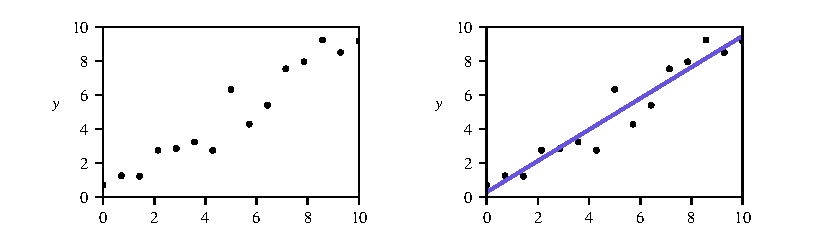
\includegraphics{simple-lin-reg}
    \caption{A dataset with a clear linear trend (left). A line which seems to fit the apparent linear relationship (right).}
    \label{fig:simple-lin-reg}
\end{figure}

Our eyes are naturally able to detect the very clear trend in this data. If we were given a datapoint $\bm x^*$, not necessarily in our training dataset, how would we predict its target value $y^*$? We would first fit a line to our data, as in \autoref{fig:simple-lin-reg} (right), and then we select $\hat y^*$ according to the point $(\bm x^*, \hat y^*)$ on the line.

That is the entirety of linear regression. It fits a line to our training data, and then uses that line to make predictions. In 1-dimensional input space, this manifests itself as the simple problem seen above,where  we need only find a single bias term $w_0$ (which acts as the intercept of the line) and single weight $w_1$ (which acts as the slope of the line). However, the same principle applies to higher dimensional data as well. We're always fitting the hyperplane that best predicts the data.

\begin{warning}
    Although our input data points $\bm x$ can take on multiple dimensions, our output data $y$ is always a 1-dimensional real number when dealing with regression problems.
\end{warning}


\subsection{Least squares loss}
% Now that we have some intuition for what linear regression is, a natural question arises: how do we find the optimal values for $\bm w$?
Now that we've defined our model as a weighted combination of our input variables, we need some way to choose our value of $\bm w$. To do this, we need an objective or loss function.

Recall that the objective function measures the ``goodness'' of a model. We can optimize this function to identify the best possible model for our data. Note that in the case of linear regression, our model is entirely specified by our settings of parameters $\bm w$.

An objective function will sometimes be referred to as \textit{loss}. Loss actually measures how bad a model is, and then our goal is to minimize it. It is common to think in terms of loss when discussing linear regression, and we incur loss when the hyperplane we fit is far away from our data.

So how do we compute the loss for a specific setting of $\bm w$? To do this, we often use \emph{residuals}.

\begin{definition}[residual]
    The residual is the difference between the target $y$ and prediction $\hat y = f(\bm x; \bm w)$ value that a model produces: $$y - f(\bm x; \bm w) = y - \bm w\T \bm x.$$
\end{definition}

Commonly, loss is a function of the residuals produced by a model. For example, you can imagine taking the absolute value of all of the residuals and adding those up to produce a measurement of loss. This is referred to as \textit{L1 loss}. Or, you might square all of the residuals and then add those up to produce loss, which is called \textit{L2 loss} or \textit{least squares loss}. You might also use some combination of L1 and L2 loss. For the most part, these are the two most common forms of loss you will see when discussing linear regression.

\begin{definition}[least squares loss]
    The least squares loss of a model $\bm w$ over a labelled dataset $\mathcal D$ is the sum of the squared residuals or ``losses'': $$\mathcal L(\bm w; \mathcal D) := \frac12 \sum_{(\bm x, y) \in \mathcal D} (y - f(\bm x; \bm w))^2.$$
\end{definition}

\begin{warning}
    Notice that our summation happens over the dataset: this means that for same model $\bm w$ can have very different losses depending on the training dataset collected. This is why we hope our training dataset is an accurate representation of the entire global dataset of possible inputs yet seen. We often will leave this out as implicit, simply using $\mathcal L(\bm w)$.
\end{warning}

When minimized, these distinct measurements of loss will produce solutions for $\bm w$ that have different properties. For example, L2 loss is not robust to outliers due to the fact that we are squaring residuals. Furthermore, L2 loss will produce only a single solution while L1 loss can potentially have many equivalent solutions. Finally, L1 loss produces unstable solutions, meaning that for small changes in our dataset, we may see large changes in our solution $\bm{w}$.

Loss is a concept that we will come back to very frequently in the context of supervised machine learning methods. Before exploring exactly how we use loss to fit a line, let's consider least squares loss in greater depth.


There is a satisfying statistical interpretation for using this loss function which we will explain later in this chapter, but for now it will suffice to discuss some of the properties of this loss function that make it desirable.

First, notice that it will always take on positive values. This is convenient because we can focus exclusively on minimizing our loss, and it also allows us to combine the loss incurred from different data points without worrying about them cancelling out.

A more subtle but enormously important property of this loss function is that it is strongly convex. This means we also know that there exists a unique global minimum where the derivative of the function is equal to 0, as seen in \autoref{fig:lin-reg-minima}. This is in part credit to the fact that strongly convex functions are continuously differentiable. In contrast, L1 loss is not continuously differentiable over the entirety of its domain.

\begin{figure}
    \centering
    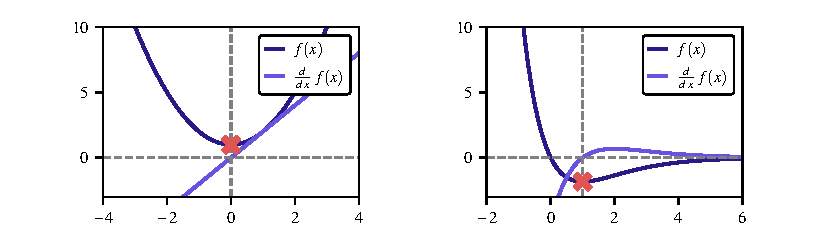
\includegraphics{lin-reg-minima}
    \caption{Strongly convex functions are minimized where their derivative 0.}
    \label{fig:lin-reg-minima}
\end{figure}

\subsection{Solving for Optimal Weights Analytically}
Now that we have our least squares loss function, we can finally begin to fit a line to our data. Our goal is to find the optimal set of weights $\bm{w}^*$ with respect to a particular labelled training dataset $\mathcal{D}$: $$\bm{w}^* := \argmin_w \mathcal{L}(\bm{w}; \mathcal{D}).$$

For convinience, we can concatenate our dataset $\mathcal{D} := \{(\bm{x}_i, y_i)\}_{i=1}^{n}$ as $\mathcal{D} = (\bm{X}, \bm{y})$ where $\bm{X} := [\bm{x}_1, \ldots, \bm{x}_n]\T \in \mathbb{R}^{n \times d}$ and $\bm{y} := [y_1, \ldots, y_n]\T$. The matrix $\bm{X}$ is commonly referred to as the \emph{design matrix}.

\begin{derivation}[least squares optimal weights]
    \label{der:least-squares-derivation}
    We find the optimal weights $\bm{w}^*$ as follows:

    Start by taking the gradient of the loss with respect to our parameter $\bm{w}$: $$\nabla \mathcal{L}(\bm{w}; \mathcal D) = \sum_{n=1}^{N} (y_n - \bm{w}\T \bm{x}_n)(-\bm{x}_n).$$

    Setting this gradient to 0 and multiplying both sides by -1, we get 
    \begin{align*}
        0 &= \sum_{n=1}^{N} y_n \bm{x}_n - \sum_{n=1}^N (\bm{w}\T\bm{x}_n)\bm{x}_n \\
        &= \sum_{n=1}^{N} y_n \bm{x}_n - \sum_{n=1}^N \bm{x}_n(\bm{x}_n\T\bm{w}).
    \end{align*}
    
    We get this last line by noticing that $(\bm{w}\T\bm{x}_n)\bm{x}_n = (\bm{x}_n\T\bm{w})\bm{x}_n = \bm{x}_n(\bm{x}_n\T\bm{w})$. (This is because $a\T=a$ and $a\bm{v}=\bm{v}a$ for any scalar $a$ and vector $\bm{v}$).

    At this point, it is convenient to rewrite these summations as matrix operations. Using the design matrix $\bm{X}$ and target values $\bm{y}$, we have
    \begin{align*}
    \bm{X}\T\bm{y}=\sum_{n=1}^N y_n \bm{x}_n, \quad
    \bm{X}\T\bm{X}\bm{w}=\sum_{n=1}^N\bm{x}_n(\bm{x}_n\T\bm{w}).
    \end{align*}

    After substituting, $$0 = \bm{X}\T\bm{y} - \bm{X}\T\bm{X}\bm{w},$$

    we can solve for $\bm{w}^*$:
    \begin{equation}
        \label{eq:least-squares-solved-for-w}
        \bm{w}^* = (\bm{X}\T \bm{X})^{-1} \bm{X}\T \bm{y}.
    \end{equation}

    For this to be well defined we need $\bm{X}$ to have full column rank (features are not colinear) so that $\bm{X}\T \bm{X}$ is positive definite and the inverse exists.
\end{derivation}

The quantity $(\bm{X}\T\bm{X})^{-1}\bm{X}\T$ in \autoref{der:least-squares-derivation} has a special name: the \emph{Moore-Penrose pseudoinverse}. You can think of it as the generalization of matrix inversion for non-square matrices.

\subsection{Solving for Optimal Weights Geometrically}
Another common interpretation of linear regression is that of a projection of our targets, $\bm{y}$, onto the column space of our inputs $\bm{X}$. This can be useful for building intuition.

We showed above that the quantity $(\bm{X}\T\bm{X})^{-1}\bm{X}\T$ can be thought of as the pseudoinverse for our inputs $\bm{X}$. Let's now consider the case where $\bm{X}$ is square and the pseudoinverse is equal to the true inverse: $\bm{X}^{-1} = (\bm{X}\T\bm{X})^{-1}\bm{X}\T$. With this assumption,
\begin{align*}
    \bm{w}^* &= (\bm{X}\T\bm{X})^{-1}\bm{X}\T\bm{y} \\
    &= \bm{X}^{-1}\bm{y}.
\end{align*}

We can recover our target values $\bm{y}$ by multiplying either side by $\bm{X}$:
\begin{align*}
    \bm{X}\bm{w}^* &= \bm{X}\bm{X}^{-1}\bm{y} \\
    \bm{X}\bm{w}^* &= \bm{y}
\end{align*}

We were able to recover our targets $\bm{y}$ exactly because $\bm{X}$ is an invertible tranformation. However, in the general case where $\bm{X}$ is not invertible and we have to use the approximate pseudoinverse $(\bm{X}\T\bm{X})^{-1}\bm{X}\T$, we instead recover $\hat{\bm{y}}$:
\begin{align*}
    \bm{X}\bm{w}^* = \bm{X}(\bm{X}\T\bm{X})^{-1}\bm{X}\T\bm{y} \\
    \bm{X}\bm{w}^* = \hat{\bm{y}}
\end{align*}
where $\hat{\bm{y}}$ can be thought of as the closest projection of $\bm{y}$ onto the column space of $\bm{X}$.

This motivates the intuition that $\bm{w}^*$ is the set of coefficients that best transforms our input space $\bm{X}$ into our target values $\bm{y}$.

\section{Probabalistic Linear Regression}
We've thus far been discussing linear regression exclusively in terms of a loss function that helps us fit a set of weights to our data. In particular, we have been working with least squares, which has nice properties that make it a reasonable loss function.

In a very satisfying fashion, least squares also has a statistical foundation. In fact, you can recover the least squares loss function purely from a statistical derivation that we present here.

Consider our dataset $\mathcal D = \{(\bm x_i, y_i)\}_{i = 1}^{n}$, where $\bm{x}_n \in\mathbb R^d$ and $y \in\mathbb{R}$. Let's imagine that every label $y_i$ was generated from a probability distribution determined by $\bm x_i$ in some way. Namely, imagine $y_i$ is a realization of the random variable
\begin{align*}
    \mathrm y_i \sim \mathcal{N}(\bm w\T \bm x_n, \sigma^2).
\end{align*}
The PDF of the r.v. $\mathrm y_i$ is hence given by:
\begin{equation}
    \label{eq:normal-over-w}
    P(\mathrm y_i = y_i) = p(y_i; \bm x_i, \bm w) = \mathcal{N}(y_i; \bm w\T \bm x_i, \sigma^2)
\end{equation}

The interpretation of the story we are imposing here is that each datapoint's label is drawn randomly. This story makes sense: if a doctor measures a patient's blood pressure, there is randomness associated with the imperfections of the instruments with which the measurements were taken. By assuming each label $\mathrm y_i$ is distributed as Gaussian with mean $\bm w\T \bm x_i$, we are assuming that it is unlikely to see $y_i$ far from $\bm w\T \bm x_i$.

Also notice that $\sigma^2$ is fixed. Namely, $p(y_i; \bm x_i, \bm w)$ is not parametrized by $\sigma^2$. It absolutely can be. In fact, we can assume a different variance for every single training datapoint. But, assuming they all have the same variance is a common and safe assumption (and we will see why).

\begin{warning}
    Notice the notational difference between the r.v. $\mathrm y$ (normal case) and the realization $y$ (italics). Also notice the difference between $\mathcal{N}(\mu, \sigma^2)$, the Gaussian distribution with mean $\mu$ and variance $\sigma^2$, and its the PDF $$\mathcal{N}(x; \mu, \sigma^2) := \frac{1}{\sqrt{2 \pi \sigma^2}} \exp\left( -\frac12 \frac{(x-\mu)^2}{\sigma^2} \right).$$
\end{warning}

\subsection{Maximum likelihood estimation}

As before, how do we solve for the optimal weights $\bm w$? One approach we can take is to choose the weights $\bm w$ which maximize the likelihood of observing our labels $\bm y$. This technique is known as \textit{maximum likelihood estimation}.

The likelihood of some weights $\bm{w}$ is the probability of observing our $\mathcal D := (\bm{X}, \bm{y})$ given those weights: $$\ell(\bm{w}; \mathcal D) := \prod_{i=1}^n p(y_i; \bm{x}_i, \bm{w}).$$ Since we assume the training datapoints are independent, we simply multiplied the probabilities $P(\mathrm y_i = y_i)$ together. Our goal is to find the optimal model $\bm{w}^*$ which maximizes the likelihood of our training data: $$\bm{w}^* := \argmax_{\bm{w}} \ell(\bm{w}; \mathcal D).$$

\begin{derivation}[MLE optimal weights]
    The likelihood of our model $\bm{w}$ given a dataset $\mathcal D = (\bm{X}, \bm{y})$ and a fixed variance $\sigma^2$ is given by
    \begin{align*}
        p(\bm{y} \mid \bm{X}, \bm{w}, \beta) = \prod_{n=1}^{N} \mathcal{N}(\bm{w}\T\bm{x}_n, \beta^{-1})
    \end{align*}
    We then take the logarithm of the likelihood, and since the logarithm is a strictly increasing, continuous function, this will not change our optimal weights $\bm{w}$:
    \begin{align*}
        \ln{p(\bm{y} \mid \bm{X}, \bm{w}, \beta)} = \sum_{n=1}^{N} \ln{\mathcal{N}(\bm{w}\T\bm{x}_n, \beta^{-1})}
    \end{align*}
    Using the density function of a univariate Gaussian:
    \begin{align*}
        \ln{p(\bm{y} \mid \bm{X}, \bm{w}, \beta)} &= \sum_{n=1}^{N} \ln{\frac{1}{\sqrt{2\pi\beta^{-1}}} e^{-(y_n - \bm{w}\T\bm{x}_n)^2 / 2\beta^{-1}}} \\
        &= \frac{N}{2}\ln{\beta} - \frac{N}{2}\ln{(2\pi)} - \frac{\beta}{2} \sum_{n=1}^{N} (y_n - \bm{w}\T\bm{x}_n)^2
    \end{align*}

    Notice that this is a quadratic function in $\bm{w}$, which means that we can solve for it by taking the derivative with respect to $\bm{w}$, setting that expression to 0, and solving for $\bm{w}$:
    \begin{align*}
      \frac{\partial \ln{p(\bm{y} | \bm{X}, \bm{w}, \beta)}}{\partial \bm{w}} & = -  \beta \sum_{n=1}^{N} (y_n - \bm{w}\T\bm{x}_n)(-\bm{x}_n)
      \\
      \Leftrightarrow \quad & 
      \sum_{n=1}^{N} y_n \bm{x}_n - \sum_{n=1}^N (\bm{w}\T\bm{x}_n)\bm{x}_n=0.
    \end{align*}

    Notice that this is exactly the same form as Equation \ref{least-squares-solving-for-w}. Solving for $\bm{w}$ as before, we have:
    \begin{equation}
        \label{eq:mle-solved-for-w}
        \bm{w}^* = (\bm{X}\T\bm{X})^{-1}\bm{X}\T\bm{y}
    \end{equation}
\end{derivation}

Notice that our final solution is exactly the same form as the solution in \autoref{eq:least-squares-solved-for-w}, which we solved for by minimizing the least squares loss! The takeaway here is that minimizing a least squares loss function is equivalent to maximizing the probability under the assumption of a linear model with Gaussian noise.

\section{Kernel Regression}
Occasionally, linear regression will fail to recover a good solution for a dataset. While this may be because our data doesn't actually have predictive power, it might also just indicate that our data is provided in a format unsuitable for linear regression. This section explores that problem, in particular focusing on how we can manipulate the flexibility of our models to make them perform better.

\subsection{Basis Functions}
There are some situations where linear regression is not the best choice of model for our input data $\bm{X}$. Because linear regression only scales and combines input variables, it is unable to apply more complex transformations to our data such as a \textit{sin} or square root function. In those situations where we need to transform our input variable somehow prior to performing linear regression (which is known as moving our data into a new \textit{basis}), we can apply a \textbf{basis function}.

\begin{definition}[basis function]
    Typically denoted by the symbol $\phi(\cdot)$, a basis function is a transformation applied to an input data point $\bm{x}$ to move our data into a different \textit{input basis}, which is another phrase for \textit{input domain}. \\

    For example, consider our original data point:
    \begin{align*}
    \bm{x} = (x^{(1)}, x^{(2)})'
    \end{align*}
    We may choose our basis function $\phi(\bm{x})$ such that our transformed data point in its new basis is:
    \begin{align*}
        \phi(\bm{x}) = (x^{(1)}, {x^{(1)}}^2, x^{(2)}, \sin(x^{(2)}))'
    \end{align*}

    Using a basis function is so common that we will sometimes describe our input data points as $\boldsymbol{\phi} = (\phi^{(1)}, \phi^{(2)}, ..., \phi^{(D)})'$.
\end{definition}

\begin{warning}
    The notation $\bm{x} = (x^{(1)}, x^{(2)})'$ is a way to describe the dimensions of a single data point $\bm{x}$. The term $\bm{x}^{(1)}$ is the first dimension of a data point $\bm{x}$, while $\bm{x}_1$ is the first data point in a dataset.
\end{warning}

Basis functions are very general - they could specify that we just keep our input data the same. As a result, it's common to rewrite the least squares loss function from Equation \ref{least-squares-loss-fn} for linear regression in terms of the basis function applied to our input data:

\begin{equation} \label{least-squares-loss-fn-w-basis}
    \mathcal{L}(\bm{w}) = \frac{1}{2} \sum_{n=1}^{N} (y_n - \bm{w}\T\boldsymbol{\phi}_n)^2
\end{equation}

To motivate why we might need basis functions for performing linear regression, let's consider this graph of 1-dimensional inputs $\bm{X}$ along with their target outputs $\bm{y}$, presented in Figure \ref{fig:lin-reg-no-basis-fn}.

\begin{figure}
    \centering
    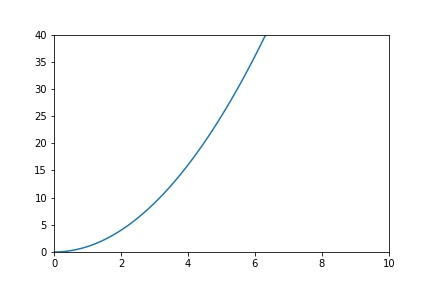
\includegraphics[width=0.5\paperwidth]{old/lin_reg_no_basis_fn_GEN.jpg}
    \caption{Data with no basis function applied.}
    \label{fig:lin-reg-no-basis-fn}
\end{figure}

As we can see, we're not going to be able to fit a good line to this data. The best we can hope to do is something like that of Figure \ref{fig:lin-reg-no-basis-fn-fitted}.

\begin{figure}
    \centering
    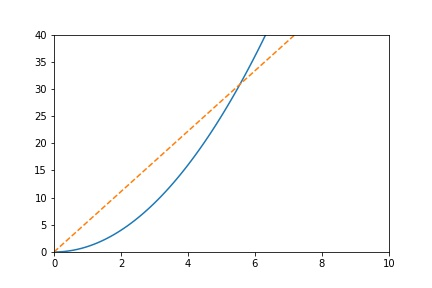
\includegraphics[width=0.5\paperwidth]{old/lin_reg_no_basis_fn_fitted_GEN.jpg}
    \caption{Data with no basis function applied, attempt to fit a line.}
    \label{fig:lin-reg-no-basis-fn-fitted}
\end{figure}

However, if we just apply a simple basis function to our data, in this case the square root function, $\phi(\bm{x}) = (\sqrt{x_1})'$, we then have the red line in Figure \ref{fig:lin-reg-w-basis-fn-fitted}. We now see that we can fit a very good line to our data, thanks to basis functions.

\begin{figure}
    \centering
    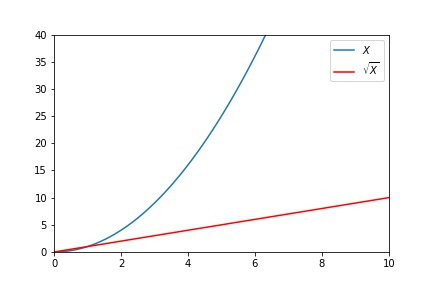
\includegraphics[width=0.5\paperwidth]{old/lin_reg_w_basis_fn_GEN.jpg}
    \caption{Data with square root basis function applied.}
    \label{fig:lin-reg-w-basis-fn-fitted}
\end{figure}

Still, the logical question remains: how can I choose the appropriate basis function? This toy example had a very obviously good basis function, but in general with high-dimensional, messy input data, how do we choose the basis function we need?

The answer is that this is not an easy problem to solve. Often, you may have some domain specific knowledge that tells you to try a certain basis, such as if you're working with chemical data and know that an important equation involves a certain function of one of your inputs. However, more often than not we won't have this expert knowledge either. Later, in the chapter on neural networks, we will discuss methods for discovering the best basis functions for our data automatically.

\subsection{Regularization}
When we introduced the idea of basis functions above, you might have wondered why we didn't just try adding many basis transformations to our input data to find a good transformation. For example, we might use this large basis function on a $D$-dimensional data point $\bm{z}$:
\begin{align*}
    \phi(\bm{z}) = (z^{(1)}, {z^{(1)}}^{2}, ..., {z^{(1)}}^{100}, z^{(2)}, {z^{(2)}}^{2}, ..., {z^{(2)}}^{100}, ..., z^{(D)}, {z^{(D)}}^{2}, ..., {z^{(D)}}^{100})'
\end{align*}
where you can see that we expand the dimensions of the data point to be 100 times its original size.

Let's say we have an input data point $\bm{x}$ that is 1-dimensional, and we apply the basis function described above, so that after the transformation each data point is represented by 100 values. Say we have 100 data points on which to perform linear regression, and because our transformed input space has 100 values, we have 100 parameters to fit. In this case, with one parameter per data point, it's possible for us to fit our regression line perfectly to our data so that we have no loss! But is this a desirable outcome? The answer is no, and we'll provide a visual example to illustrate that.

Imagine Figure \ref{fig:data-set-scattered} is our dataset. There is a very clear trend in this data, and you would likely draw a line that looks something like that of Figure \ref{fig:data-set-natural-fit} to fit it.

\begin{figure}
    \centering
    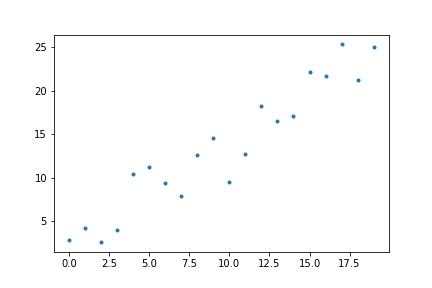
\includegraphics[width=0.5\paperwidth]{old/data_set_scattered_GEN.jpg}
    \caption{Dataset with a clear trend and Gaussian noise.}
    \label{fig:data-set-scattered}
\end{figure}

\begin{figure}
    \centering
    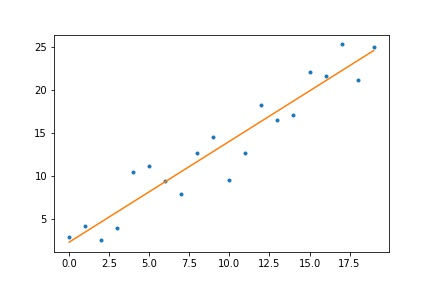
\includegraphics[width=0.5\paperwidth]{old/data_set_natural_fit_GEN.jpg}
    \caption{Natural fit for this dataset.}
    \label{fig:data-set-natural-fit}
\end{figure}

However, imagine we performed a large basis transformation like the one described above. If we do that, it's possible for us to fit our line perfectly, threading every data point, like that in Figure \ref{fig:data-set-unnatural-fit}.

\begin{figure}
    \centering
    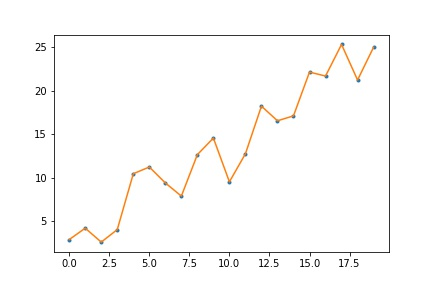
\includegraphics[width=0.5\paperwidth]{old/data_set_unnatural_fit_GEN.jpg}
    \caption{Unnatural fit for this dataset.}
    \label{fig:data-set-unnatural-fit}
\end{figure}

Let's see how both of these would perform on new data points. With our first regression line, if we have a new data point $\bm{x} = (10)'$, we would predict a target value of $\bm{14.1}$, which most people would agree is a pretty good measurement. However, with the second regression line, we would predict a value of $\bm{9.5}$, which most people would agree does not describe the general trend in the data. So how can we handle this problem elegantly?

Examining our loss function, we see that right now we're only penalizing predictions that are not correct in training. However, what we ultimately care about is doing well on new data points, not just our training set. This leads us to the idea of \textbf{generalization}.

\begin{definition}[generalization]
    Generalization is the ability of a model to perform well on new data points outside of the training set.
\end{definition}

A convoluted line that matches the noise of our training set exactly isn't going to generalize well to new data points that don't look exactly like those found in our training set. If wish to avoid recovering a convoluted line as our solution, we should also penalize the total size of our weights $\bm{w}$. The effect of this is to discourage many complex weight values that produce a messy regression line. By penalizing large weights, we favor simple regression lines like the one in Figure \ref{fig:data-set-natural-fit} that take advantage of only the most important basis functions.

The concept that we are introducing, penalizing large weights, is an example of what's known as \textbf{regularization}, and it's one that we will see come up often in different machine learning methods.

\begin{definition}[regularization]
    Applying penalties to parameters of a model.
\end{definition}

There is obviously a tradeoff between how aggressively we regularize our weights and how tightly our solution fits to our data, and we will formalize this tradeoff in the next section. However, for now, we will simply introduce a regularization parameter $\lambda$ to our least squares loss function:

\begin{equation} \label{least-squares-loss-fn-w-regularization}
    \mathcal{L}(\bm{w}) = \frac{1}{2} \sum_{n=1}^{N} (y_n - \bm{w}\T\boldsymbol{\phi}_n)^2 + \frac{\lambda}{2}\bm{w}^{\top}\bm{w}
\end{equation}

The effect of $\lambda$ is to penalize large weight parameters. The larger $\lambda$ is, the more we will favor simple solutions. In the limit $\lim_{\lambda\to\infty} \mathcal{L}(\bm{w})$, we will drive all weights to 0, while with a nonexistant $\lambda = 0$ we will apply no regularization at all. Notice that we're squaring our weight parameters - this is known as \textit{L2 norm regularization} or \textbf{ridge regression}. While L2 norm regularization is very common, it is just one example of many ways we can perform regularization.

To build some intuition about the effect of this regularization parameter, examine Figure \ref{fig:ridge-reg-diff-values}. Notice how larger values of $\lambda$ produce less complex lines, which is the result of applying more regularization. This is very nice for the problem we started with - needing a way to choose which basis functions we wanted to use. With regularization, we can select many basis functions, and then allow regularization to `prune' the ones that aren't meaningful (by driving their weight parameters to 0). While this doesn't mean that we should use as many basis transformations as possible (there will be computational overhead for doing this), it does allow us to create a much more flexible linear regression model without creating a convoluted regression line.

\begin{figure}
    \centering
    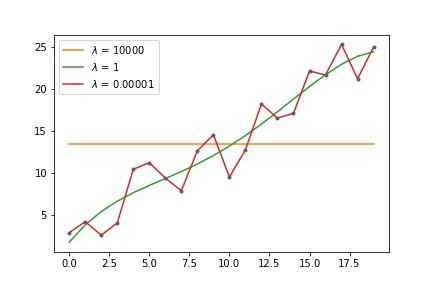
\includegraphics[width=0.5\paperwidth]{old/diffregvalues_GEN.jpg}
    \caption{Effect of different regularization parameter values on final regression solution.}
    \label{fig:ridge-reg-diff-values}
\end{figure}

\subsection{Generalizing Regularization}
We've thus far only discussed one form of regularization: ridge regression. Remember that under ridge regression, the loss function takes the form:
\begin{align*}
    \mathcal{L}(\bm{w}) = \frac{1}{2} \sum_{n=1}^{N} (y_n - \bm{w}\T\boldsymbol{\phi}_n)^2 + \frac{\lambda}{2}\bm{w}^{\top}\bm{w},
\end{align*}
%
where the $(\lambda/2)\bm{w}\T\bm{w}$ term is for the regularization. We can generalize our type of regularization by writing it as:
\begin{align*}
    \mathcal{L}(\bm{w}) = \frac{1}{2} \sum_{n=1}^{N} (y_n - \bm{w}\T\boldsymbol{\phi}_n)^2 + \frac{\lambda}{2}\big|\big|\bm{w}\big|\big|_h^{h}
\end{align*}
where $h$ determines the type of regularization we are using and thus the form of the optimal solution that we recover. For example, if $h=2$ then we add $\lambda/2$ times the square of the L2 norm.
%x
The three most commonly used forms of regularization are lasso, ridge, and elastic net. \newline \newline
\textbf{Ridge Regression} \newline
This is the case of $h = 2$, which we've already discussed, but what type of solutions does it tend to recover? Ridge regression prevents any individual weight from growing too large, providing us with solutions that are generally moderate. \newline \newline
\textbf{Lasso Regression} \newline
Lasso regression is the case of $h = 1$. Unlike ridge regression, lasso regression will drive some parameters $w_i$ to zero if they aren't informative for our final solution. Thus, lasso regression is good if you wish to recover a sparse solution that will allow you to throw out some of your basis functions. You can see the forms of ridge and lasso regression functions in Figure \ref{fig:ridge-and-lasso-reg-fn-form}.
If you think about how Lasso is L1 Norm (absolute value) and Ridge is L2 Norm (squared distance), you can think of those shapes as being the set of points $(w_1,w_2)$ for which the norm takes on a constant value.
%Just like a circle is a set of points at constant radius from its center, a rotated square with its vertices at [1,0], [-1,0], [0,1], [0,-1] is the set of 2D points with sum of abs values equal to 1.  
%
\newline
\newline

\textbf{Elastic Net} \newline
Elastic net is a middle ground between ridge and lasso regression, which it achieves by using a linear combination of the previous two regularization terms. Depending on how heavily each regularization term is weighted, this can produce results on a spectrum between lasso and ridge regression. \\

\begin{figure}
    \centering
    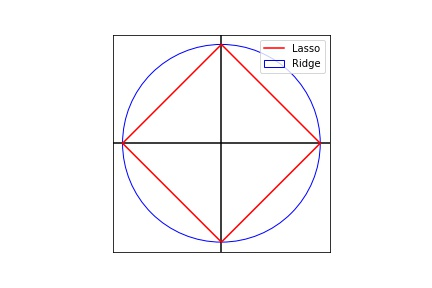
\includegraphics[width=0.5\paperwidth]{old/ridgeandlassoreg_GEN.jpg}
    \caption{Form of the ridge (blue) and lasso (red) regression functions.}
    \label{fig:ridge-and-lasso-reg-fn-form}
\end{figure}


\subsection{Bayesian Regularization} \label{bayesian-regularization-section}
We've seen regularization in the context of loss functions, where the goal is to penalize large weight values. How does the concept of regularization apply to Bayesian linear regression?

The answer is that we can interpret regularizing our weight parameters as adding a prior distribution over $\bm{w}$. Note that this is a different conception of regularization than we saw in the previous section. In the Bayesian framework, we are averaging over different models specified by different values of $\bm{w}$. Therefore, in this context regularization entails weighting models with smaller values of $\bm{w}$ more heavily.

\begin{derivation}[Bayesian Regularization Derivation]
    Because we wish to shrink our weight values toward 0 (which is exactly what regularization does), we will select a Normal prior with mean 0 and variance $\boldsymbol{S}_0^{-1}$:
    \begin{align*}
        \bm{w} \sim \mathcal{N}(0, \boldsymbol{S}_0^{-1}\bm{I})
    \end{align*}
    Remember from Equation \ref{normal-over-w} that the distribution over our observed data is Normal as well, written here in terms of our entire dataset:
    \begin{align*}
        p(\bm{y} | \bm{X}, \bm{w}, \beta) = \mathcal{N}(\bm{X}\bm{w}, \beta^{-1}\bm{I})
    \end{align*}
    % We want to combine the likelihood and the prior to recover the posterior distribution of $\bm{w}$, which follows directly from Bayes' Theorem:
    \begin{align*}
        \underbrace{p(\bm{w}|\bm{X},\bm{y}, \beta)}_{\text{posterior}} \propto \underbrace{p(\bm{y}| \bm{X}, \bm{w}, \beta)}_{\text{likelihood}}\underbrace{p(\bm{w})}_{\text{prior}}
    \end{align*}
    We now wish to find the value of $\bm{w}$ that maximizes the posterior distribution. We can maximize the log of the posterior with respect to $\bm{w}$, which simplifies the problem slightly:
    \begin{align*}
        \ln{p(\bm{w}|\bm{X},\bm{y}, \beta)} \propto \ln{p(\bm{y}| \bm{X}, \bm{w}, \beta)} + \ln{p(\bm{w})}
    \end{align*}
    Let's handle $\ln{p(\bm{y}| \bm{X}, \bm{w}, \beta)}$ first:
    \begin{align*}
        \ln{p(\bm{y}| \bm{X}, \bm{w}, \beta)} &= \ln{\prod_{n=1}^{N} \mathcal{N}(y_n | \bm{w}\T \bm{x}_n, \beta^{-1})} \\
        &= \ln{\prod_{n=1}^{N} \frac{1}{\sqrt{2\pi\beta^{-1}}} \exp{\bigg\{-\frac{\beta}{2}(y_n - \bm{w}\T \bm{x}_n)^2\bigg\}}} \\
        &= \bm{C} -\frac{\beta}{2}\sum_{n=1}^{N} (y_n - \bm{w}\T \bm{x}_n)^2 + \frac{1}{\sqrt{2\pi\beta^{-1}}}
    \end{align*}
    where $\bm{C}$ collects the constant terms that don't depend on $\bm{w}$. Let's now handle $\ln{p(\bm{w})}$:
    \begin{align*}
        \ln{p(\bm{w})} &= \ln{\mathcal{N}(0, \boldsymbol{S}_0^{-1}\bm{I})} \\
        &= \ln{\frac{1}{(|2\pi\boldsymbol{S}_0^{-1}\bm{I}|)^{\frac{1}{2}}} \exp{\bigg\{-\frac{\boldsymbol{S}_0}{2} \bm{w}\T\bm{w}\bigg\}}} \\
        &= \bm{C} -\frac{\boldsymbol{S}_0}{2} \bm{w}\T\bm{w}
    \end{align*}
    combining the terms for $\ln{p(\bm{y}| \bm{X}, \bm{w}, \beta)}$ and $\ln{p(\bm{w})}$:
    \begin{align*}
        \ln{p(\bm{w}|\bm{X},\bm{y}, \beta)} = -\frac{\beta}{2}\sum_{n=1}^{N} (y_n - \bm{w}\T \bm{x}_n)^2 - \frac{\boldsymbol{S}_0}{2} \bm{w}\T\bm{w}
    \end{align*}
    dividing by a positive constant $\beta$:
    \begin{align*}
        \ln{p(\bm{w}|\bm{X},\bm{y}, \beta)} = -\frac{1}{2}\sum_{n=1}^{N} (y_n - \bm{w}\T \bm{x}_n)^2 - \frac{\boldsymbol{S}_0}{\beta}\frac{1}{2} \bm{w}\T\bm{w}
    \end{align*}
    Notice that maximizing the posterior probability is equivalent to minimizing the sum of squared errors $(y_n - \bm{w}\T \bm{x}_n)^2$ and the regularization term $\bm{w}\T\bm{w}$.
\end{derivation}

\textbf{The interpretation of this is that adding a prior over the distribution of our weight parameters $\bm{w}$ and then maximizing the resulting posterior distribution is equivalent to adding a regularization term where $\lambda = \frac{\boldsymbol{S}_0}{\beta}$}

\section{Model Selection}
\subsection{Bias-Variance Tradeoff and Decomposition}
Now that you know about regularization, you might have some intuition for why we need to find a balance between complex and simple regression solutions. A complex solution, while it might fit all of our training data, may not generalize well to future data points. On the other hand, a line that is too simple might not vary enough to provide good predictions at all. This phenomenon is not unique to linear regression- it's actually a very fundamental concept in machine learning that's known as the \textbf{bias-variance tradeoff}.

\begin{definition}[Bias-Variance Tradeoff]
    When constructing machine learning models, we have a choice somewhere on a spectrum between two extremes: fitting exactly to our training data or not varying in response to our training data at all. The first extreme, fitting all of our training data, is a situation of high \textit{variance}, because our output changes heavily in reponse to our input data (see the red line in Figure \ref{fig:ridge-reg-diff-values}). At the other extreme, a solution that doesn't change in response to our training data at all is a situation of high \textit{bias} (see the yellow line in Figure \ref{fig:ridge-reg-diff-values}). This means our model heavily favors a specific form regardless of the training data, so our target outputs don't fluctuate between distinct training sets.
\end{definition}

Obviously a good solution will fall somewhere in between these two extremes of high variance and high bias. Indeed, we have techniques like regularization to help us balance the two extremes (improving generalization), and we have other techniques like \textit{cross-validation} that help us determine when we have found a good balance (measuring generalization).

\begin{warning}
    In case you are not familiar with the terms \textit{bias} and \textit{variance}, we provide their statistical definitions here:
    \begin{align*}
        \text{bias($\theta$)} = \mathrm{E}[\theta] - \theta
    \end{align*}
    \begin{align*}
        \text{variance($\theta$)} = \mathrm{E}[(\theta - \mathrm{E}[\theta])^{2}]
    \end{align*}
\end{warning}

Before we discuss how to effectively mediate between these opposing forces of error in our models, we will first show that the bias-variance tradeoff is not only conceptual but also has probabilistic underpinnings. Specifically, any loss that we incur over our training set using a given model can be described in terms of bias and variance, as we will demonstrate now.

% \begin{derivation}[bias-variance decomposition]
%     Let's begin by asserting that we have a model $f(\cdot)$ that makes a prediction of our target $y$ given input data point $\bm{x}$. We wish to break down the squared error of $f$ into terms involving bias and variance. \\

%     Start with the expected squared error (MSE), where the expectation is taken with respect to both our dataset $\bm{D}$ (variation in our modeling error comes from what dataset we get), which is a random variable of $(\bm{x}, y)$ pairs sample from a distribution $F$, and our conditional distribution $y | \bm{x}$ (there may be additional error because the data are noisy):
%     \begin{align*}
%         \textit{MSE} = \mathrm{E}_{\bm{D},y|x}[(y - f_\bm{D}(\bm{x}))^{2}]
%     \end{align*}
%     where we use the notation $f_\bm{D}$ to explicitly acknowledge the dependence of our fitted model $f$ on the dataset $\bm{D}$.  For reasons that will become clear in a few steps, add and subtract our target mean $\bar{y}$, which is the true conditional mean given by $\bar{y} = \mathrm{E}_{y|\bm{x}}[y]$, inside of the squared term:
%     \begin{align*}
%         \textit{MSE} = \mathrm{E}_{\bm{D},y|x}[(y - \bar{y} + \bar{y} - f_\bm{D}(\bm{x}))^{2}]
%     \end{align*}
%     Group together the first two terms and the last two terms:
%     \begin{align*}
%         \textit{MSE} = \mathrm{E}_{\bm{D},y|x}[((y - \bar{y}) + (\bar{y} - f_\bm{D}(\bm{x})))^{2}]
%     \end{align*}
%     Expanding this expression and using linearity of expectation:
%     \begin{equation} \label{bias-variance-intermediate-1}
%         \textit{MSE} = \mathrm{E}_{\bm{D},y|x}[(y - \bar{y})^{2}] + \mathrm{E}_{\bm{D},y|x}[(\bar{y} - f_\bm{D}(\bm{x}))^{2}] + 2\mathrm{E}_{\bm{D},y|x}[(y - \bar{y})(\bar{y} - f_\bm{D}(\bm{x}))]
%     \end{equation}
%     Let's examine the last term, $2\mathrm{E}[(y - \bar{y})(\bar{y} - f_\bm{D}(\bm{x}))]$. Notice that $(\bar{y} - f_\bm{D}(\bm{x}))$ does not depend on the conditional distribution $y|\bm{x}$ at all. Thus, we are able to move one of those expecations in, which makes this term:
%     \begin{align*}
%         2\mathrm{E}_{\bm{D},y|x}[(y - \bar{y})(\bar{y} - f_\bm{D}(\bm{x}))] = 2\mathrm{E}_{\bm{D}}[\mathrm{E}_{y|\bm{x}}[(y - \bar{y})](\bar{y} - f_\bm{D}(\bm{x}))]
%     \end{align*}
%     And note that:
%     \begin{align*}
%         \mathrm{E}_{y|\bm{x}}[(y - \bar{y})] = 0
%     \end{align*}
%     Which eliminates this last term entirely:
%     \begin{align*}
%         2\mathrm{E}_{\bm{D},y|x}[(y - \bar{y})(\bar{y} - f_\bm{D}(\bm{x}))] = 2\mathrm{E}_{\bm{D}}[0 \cdot (\bar{y} - f_\bm{D}(\bm{x}))] = 0
%     \end{align*}
%     We can now write Equation \ref{bias-variance-intermediate-1} as:
%     \begin{eqnarray} \label{bias-variance-intermediate-2}
%       \textit{MSE} &= \mathrm{E}_{\bm{D},y|x}[(y - \bar{y})^{2}] + \mathrm{E}_{\bm{D},y|x}[(\bar{y} - f_\bm{D}(\bm{x}))^{2}] \\
%       &= \mathrm{E}_{y|x}[(y - \bar{y})^{2}] + \mathrm{E}_{\bm{D}}[(\bar{y} - f_\bm{D}(\bm{x}))^{2}] \nonumber
%     \end{eqnarray}
%     where we have removed expectations that do not apply (e.g. $\bar{y}$ does not depend on the dataset $\bm{D}$). 
    
%     We now have two terms contributing to our squared error. We will put aside the first term $\mathrm{E}_{y|x}[(y - \bar{y})^{2}]$, as this is unidentifiable \textit{noise} in our dataset. In other words, our data will randomly deviate from the mean in ways we cannot predict. On the other hand, we can work with the second term $\mathrm{E}_\bm{D}[(\bar{y} - f_\bm{D}(\bm{x}))^{2}]$ as it involves our model function $f(\cdot)$ \\

%     As before, for reasons that will become clear in a few steps, let's add and subtract our prediction mean $\bar{f}(\cdot) = \mathrm{E}_\bm{D}[f_\bm{D}(\bm{x})]$, which is the expectation of our model function taken with respect to our random dataset.
%     \begin{align*}
%         \mathrm{E}_\bm{D}[(\bar{y} - f_\bm{D}(\bm{x}))^{2}] = \mathrm{E}_\bm{D}[(\bar{y} - \bar{f}(\bm{x}) + \bar{f}(\bm{x}) - f_\bm{D}(\bm{x}))^{2}]
%     \end{align*}
%     Expanding this squared term, we have:
%     \begin{align*}
%         \mathrm{E}_\bm{D}[(\bar{y} - f_\bm{D}(\bm{x}))^{2}] = (\bar{y} - \bar{f}(\bm{x}))^{2} + \mathrm{E}_\bm{D}[(\bar{f}(\bm{x}) - f_\bm{D}(\bm{x}))^{2}] + 2\mathrm{E}_\bm{D}[(\bar{y} - \bar{f}(\bm{x}))(\bar{f}(\bm{x}) - f_\bm{D}(\bm{x}))]
%     \end{align*}
%     As before, the third term here is 0:
%     \begin{align*}
%         2\mathrm{E}_\bm{D}[(\bar{y} - \bar{f}(\bm{x}))(\bar{f}(\bm{x}) - f_\bm{D}(\bm{x}))] = 2(\bar{y} - \bar{f}(\bm{x}))\mathrm{E}_\bm{D}[(\bar{f}(\bm{x}) - f_\bm{D}(\bm{x}))] = 2(\bar{y} - \bar{f}(\bm{x}))(0) = 0
%     \end{align*}
%     Leaving us with these two terms:
%     \begin{align*}
%         \mathrm{E}_\bm{D}[(\bar{y} - f_\bm{D}(\bm{x}))^{2}] = (\bar{y} - \bar{f}(\bm{x}))^{2} + \mathrm{E}_\bm{D}[(\bar{f}(\bm{x}) - f_\bm{D}(\bm{x}))^{2}]
%     \end{align*}
%     Notice the form of these two terms. The first one, $(\bar{y} - \bar{f}(\bm{x}))^{2}$, is the squared \textit{bias} of our model, since it is the square of the average difference between our prediction and the true target value. The second one, $\mathrm{E}_\bm{D}[(\bar{f}(\bm{x}) - f_\bm{D}(\bm{x}))^{2}]$, is the \textit{variance} of our model, since it is the expected squared difference between our model and its average value. Thus:
%     \begin{align*}
%         \mathrm{E}_\bm{D}[(\bar{y} - f_\bm{D}(\bm{x}))^{2}] = \textit{bias}(f(\bm{x}))^{2} + \textit{variance}(f(\bm{x}))
%     \end{align*}

%     Thus, our total squared error, plugging in to Equation \ref{bias-variance-intermediate-2} can be written as:
%     \begin{align*}
%         \boxed{\textit{MSE} = \textit{noise}(\bm{x}) + \textit{bias}(f(\bm{x}))^{2} + \textit{variance}(f(\bm{x}))}
%     \end{align*}
% \end{derivation}

\newpage
The key takeaway of the bias-variance decomposition is that the controllable error in our model is given by the squared bias and variance. Holding our error constant, to decrease bias requires increasing the variance in our model, and vice-versa. In general, a graph of the source of error in our model might look something like Figure \ref{fig:bias-vs-variance}.

\begin{figure}
    \centering
    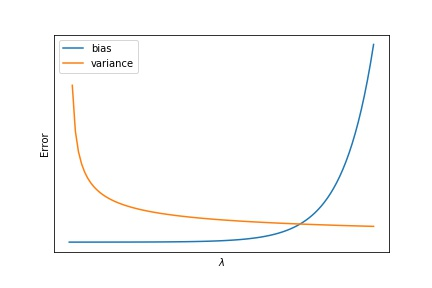
\includegraphics[width=0.5\paperwidth]{old/biasvariance_GEN.jpg}
    \caption{Bias and variance both contribute to the overall error of our model.}
    \label{fig:bias-vs-variance}
\end{figure}

For a moment, consider what happens on the far left side of this graph. Our variance is very high, and our bias is very low. In effect, we're fitting perfectly to all of the data in our dataset. This is exactly why we introduced the idea of regularization from before - we're fitting a very convoluted line that is able to pass through all of our data but which doesn't generalize well to new data points. There is a name for this: $\bm{overfitting}$.

\begin{definition}[overfitting]
    A phenomenon where we construct a convoluted model that is able to predict every point in our dataset perfectly but which doesn't generalize well to new data points.
\end{definition}

The opposite idea, $\bm{underfitting}$, is what happens at the far right of the graph: we have high bias and aren't responding to the variation in our dataset at all.

\begin{definition}[underfitting]
    A phenomenon where we construct a model that doesn't respond to variation in our data.
\end{definition}

So you can hopefully now see that the bias-variance tradeoff is important to managing the problem of overfitting and underfitting. Too much variance in our model and we'll overfit to our dataset. Too much bias and we won't account for the trends in our dataset at all.

In general, we would like to find a sweet spot of moderate bias and variance that produces minimal error. In the next section, we will explore how we find this sweet spot.

\subsection{Cross-Validation}
We've seen that in choosing a model, we incur error that can be described in terms of bias and variance. We've also seen that we can regulate the source of error through regularization, where heavier regularization increases the bias of our model. A natural question then is how do we know how much regularization to apply to achieve a good balance of bias and variance?

Another way to look at this is that we've traded the question of finding the optimal number of basis functions for finding the optimal value of the regularization parameter $\lambda$, which is often an easier problem in most contexts.

One very general technique for finding the sweet spot of our regularization parameter, other hyperparameters, or even for choosing among entirely different models is known as $\bm{cross-validation}$.

\begin{definition}[cross-validation]
    A subsampling procedure used over a dataset to tune hyperparameters and avoid over-fitting. Some portion of a dataset (10-20\% is common) is set aside, and training is performed on the remaining, larger portion of data. When training is complete, the smaller portion of data left out of training is used for testing. The larger portion of data is sometimes referred to as the \textit{training set}, and the smaller portion is sometimes referred to as the \textit{validation set}.
\end{definition}

Cross-validation is often performed more than once for a given setting of hyperparameters to avoid a skewed set of validation data being selected by chance. In $\bm{K-Folds cross-validation}$, you perform cross-validation $\bm{K}$ times, allocating $\frac{1}{\bm{K}}$ of your data for the validation set at each iteration.

Let's tie this back into finding a good regularization parameter. For a given value of $\lambda$, we will incur a certain amount of error in our model. We can measure this error using cross-validation, where we train our model on the training set and compute the final error using the validation set. To find the optimal value for $\lambda$, we perform cross-validation using different values of $\lambda$, eventually settling on the value that produces the lowest final error. This will effectively trade off bias and variance, finding the value of $\lambda$ that minimizes the total error.

You might wonder why we need to perform cross-validation at all - why can't we train on the entire dataset and then compute the error over the entire dataset as well?

The answer is again overfitting. If we train over the entire dataset and then validate our results on the exact same dataset, we are likely to choose a regularization parameter that encourages our model to conform to the exact variation in our dataset instead of finding the generalizable trends. By training on one set of data, and then validating on a completely different set of data, we force our model to find good generalizations in our dataset. This ultimately allows us to pick the regularization term $\lambda$ that finds the sweet spot between bias and variance, overfitting and underfitting.

\subsection{Making a Model Choice}
Now that we're aware of overfitting, underfitting, and how those concepts relate to the bias-variance tradeoff, we still need to come back to the question of how we actually select a model. Intuitively, we are trying to find the middle ground between bias and variance: picking a model that fits our data but that is also general enough to perform well on yet unseen data. Furthermore, there is no such thing as the `right' model choice. Instead, there are only model options that are either better or worse than others. To that end, it can be best to rely on the techniques presented above, specifically cross-validation, to make your model selection. Then, although you will not be able to make any sort of guarantee about your selection being the `best' of all possible models, you can at least have confidence your model achieved the best generalizability that could be proven through cross-validation.

\subsection{Bayesian Model Averaging}
We can also handle model selection using a Bayesian approach. This means we account for our uncertainty about the true model by averaging over the possible candidate models, weighting each model by our prior certainty that it is the one producing our data. If we have $M$ models indexed by $m = 1, ..., M$, we can write the likelihood of observing our dataset $\bm{X}$ as follows:
\begin{align*}
    p(\bm{X}) = \sum_{m=1}^{M} p(\bm{X}|m)p(m)
\end{align*}
where $p(m)$ is our prior certainty for a given model and $p(\bm{X}|m)$ is the likelihood of our dataset given that model. The elegance of this approach is that we don't have to pick any particular model, instead choosing to marginalize out our uncertainty.

\section{Linear Regression Extras}
With most of linear regression under our belt at this point, it's useful to drill down on a few concepts to come to a deeper understanding of how we can use them in the context of linear regression and beyond.

\subsection{Predictive Distribution}
Remaining in the setting of Bayesian Linear Regression, we may wish to get a distribution over our weights $\bm{w}$ instead of a point estimator for it using maximum likelihood. As we saw in Section \ref{bayesian-regularization-section}, we can introduce a prior distribution over $\bm{w}$, then together with our observed data, we can produce a posterior distribution over $\bm{w}$ as desired.

\begin{derivation}[posterior predictive derivation]
    For the sake of simplicity and ease of use, we will select our prior over $\bm{w}$ to be a Normal distribution with mean $\boldsymbol{\mu}_0$ and variance $\boldsymbol{S}_0^{-1}$:
    \begin{align*}
        p(\bm{w}) = \mathcal{N}(\boldsymbol{\mu}_0, \boldsymbol{S}_0^{-1})
    \end{align*}
    Remembering that the observed data is normally distributed, and accounting for Normal-Normal conjugacy, our posterior distribution will be Normal as well:
    \begin{align*}
        p(\bm{w}|\bm{X},\bm{y}, \beta) = \mathcal{N}(\boldsymbol{\mu}_n, \boldsymbol{S}_n^{-1})
    \end{align*}
    where
    \begin{align*}
        \boldsymbol{S}_n = (\boldsymbol{S}_0^{-1} + \beta\bm{X}\T\bm{X})^{-1} \\
        \boldsymbol{\mu}_n = \boldsymbol{S}_n(\boldsymbol{S}_0^{-1}\boldsymbol{\mu}_0 + \beta\bm{X}\bm{y})
    \end{align*}

    We now have a posterior distribution over $\bm{w}$. However, usually this distribution is not what we care about. We're actually interested in making a point prediction for the target $y^*$ given a new input $\bm{x}^*$. How do we go from a posterior distribution over $\bm{w}$ to this prediction? \\

    The answer is using what's known as the \textbf{posterior predictive} over $y^*$ given by:
    \begin{equation}
    \begin{split}
        p(y^* | \bm{x}^*, \bm{X}, \bm{y}) &= \int_{\bm{w}} p(y^* | \bm{x}^*, \bm{w})p(\bm{w} | \bm{X}, \bm{y})d\bm{w} \\
        &= \int_{\bm{w}} \mathcal{N}(y^* | \bm{w}\T\bm{x}^*, \beta^{-1})\mathcal{N}(\bm{w} | \boldsymbol{\mu}_n, \boldsymbol{S}_n^{-1})d\bm{w}
    \end{split}
    \end{equation}
\end{derivation}

\textbf{The idea here is to average the probability of $y^*$ over all the possible setting of $\bm{w}$, weighting the probabilities by how likely each setting of $\bm{w}$ is according to its posterior distribution.}

\section{Conclusion}
In this chapter, we looked at a specific tool for handling regression problems known as linear regression. We've seen linear regression described in terms of loss functions, probabilistic expressions, and geometric projections, which reflects the deep body of knowledge that we have around this very common technique.

We've also discussed many concepts in this chapter that will prove useful in other areas of machine learning, particularly for other supervised techniques: loss functions, regularization, bias and variance, over and underfitting, posterior distributions, maximum likelihood estimation, and cross-validation among others. Spending time to develop an understanding of these concepts now will pay off going forward.

It may or may not be obvious at this point that we are missing a technique for a very large class of problems: those where the solution is not just a continuous, real number. How do we handle situations where we need to make a choice between different discrete options? This is the question we will turn to in the next chapter.

  % \chapter{Classification}
In the last chapter, we explored ways of predicting a continuous, real target $y \in \mathbb{R}$. In this chapter, we're going to think about a different problem where our target output is discrete. This type of problem, one where we make a prediction by choosing between finite class options, is known as \textbf{classification}.

\section{Defining the Problem}
As we did when studying regression, let's begin by thinking about the type of problems we are trying to solve. Here are a few examples of classification tasks:
\begin{enumerate}
    \item Predicting whether a given email is spam.
    \item Predicting the type of object in an image.
    \item Predicting whether a manufactured good is defective.
\end{enumerate}
The point of classification is hopefully clear: we're trying to identify the most appropriate class $\hat{y} \in \{ C_1, \ldots, C_K \}$ for an input data point $\mathbf{x} \in \mathbb{R}^D$. 
\begin{definition}[classification]
	A set of problems that seeks to make predictions about unobserved discrete target classes given observed input variables.
\end{definition}

\section{Solution Options}

There are several different means by which we can solve classification problems. We're going to discuss three in this chapter: discriminant functions, probabilistic discriminative models (e.g. logistic regression), and probabilistic generative models. Note that these are not the only methods for performing classification tasks, but they are similar enough that it makes sense to present and explore them together. Specifically, these techniques all use some linear combination of input variables to produce a class prediction. For that reason, we will refer to these techniques as \textbf{generalized linear models}.

\begin{mlcube}[generalized linear models]{Discrete}{Supervised}{Both}
	Since we are using these techniques to perform classification, generalized linear models deal with a \textbf{discrete} output domain. Second, as with linear regression, our goal is to make predictions on future data points given an initial set of data to learn from. Thus, generalized linear models are \textbf{supervised} techniques. Finally, depending on the type of generalized linear model, they can be either \textbf{probabilistic or non-probabilistic}.
\end{mlcube}

\section{Discriminant Functions}
Generalized linear models for classification come in several different flavors. The most straightforward method carries over very easily from linear regression: \textbf{discriminant functions}. As we will see, with discriminant functions we are linearly separating the input space into sections belonging to different target classes. We will explore this method first. One thing to keep in mind is that it's generally easiest to initially learn these techniques in the case where we have only two target classes, but there is typically a generalization that allows us to handle the multi-class case as well.

As with linear regression, discriminant functions $h(\mathbf{x}, \mathbf{w})$ seek to find a weighted combination of our input variables to make a prediction about the target class:
\begin{equation}
	\label{eq:basic-discriminant-fn}
	h(\mathbf{x}, \mathbf{w}) = \mathbf{w}^\top \mathbf{x}
\end{equation}
where we are using the bias trick of appending $x_0 = 1$ to all of our data points.

\subsection{Basic Setup: Binary Linear Classification}
The simplest use case for a discriminant function is when we only have two classes that we are trying to decide between: that is, $K=2$. Let's denote these two classes $C_1 = -1$ and $C_2 = +1$. Our discriminant function in \autoref{eq:basic-discriminant-fn} will then predict class $C_1$ if $h(\mathbf{x}, \mathbf{w}) < 0$ and class $C_2$ if $h(\mathbf{x}, \mathbf{w}) \geq 0$:
$$
	\hat y = 
	\begin{cases} 
    	1 & \text{if } h(\mathbf{x}, \mathbf{w}) \geq 0 \\
    	-1 & \text{if } h(\mathbf{x}, \mathbf{w}) < 0
   \end{cases}
$$
Geometrically, the linear separation between these two classes then looks like that of \autoref{fig:lin-sep-bn-classes}.
\begin{figure}
    \centering
    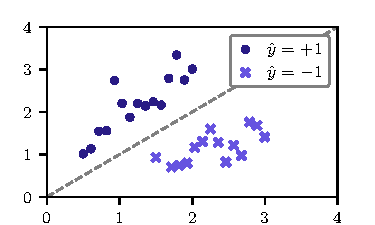
\includegraphics{lin-sep}
    \caption{Clear separation between classes.}
    \label{fig:lin-sep-bn-classes}
\end{figure}
Notice the line where our prediction switches from class 1 to class -1. This is precisely where $h(\mathbf{x}, \mathbf{w}) = 0$, and it is known as the \textbf{decision boundary}.

\begin{definition}[decision boundary]
	The decision boundary is the line that divides the input space into different target classes. It is learned from an initial data set, and then the target class of new data points can be predicted based on where they fall relative to the decision boundary. At the decision boundary, the discriminant function takes on a value of 0.
\end{definition}

\begin{warning}
	You will sometimes see the term \textbf{decision surface} in place of decision boundary, particularly if the input space is larger than two dimensions.
\end{warning}

\subsection{Multiple Classes}
Now consider the case that we have $K > 2$ classes $C_1, \dots, C_K$ to choose between. One obvious approach we might try is to use $K$ different discriminant functions that each determine whether or not a given input is in that class $C_k$. This is known as a \textbf{one-versus-all} approach, and it doesn't work properly because we end up with ambiguous regions as demonstrated in \autoref{fig:one-v-all}. Intuitively, several of the discriminator functions could claim that a data point is a part of their class, which is an undesirable result.

% \begin{figure}
%     \centering
%     \includegraphics{one-v-all}
%     \caption{Ambiguities arise from one-versus-all method.}
%     \label{fig:one-v-all}
% \end{figure}

Another obvious approach we might employ is to use $\binom{K}{2}$ discriminant functions that each determine whether a given point is more likely to be in class $C_k$ or class $C_j$. This is known as a \textit{one-versus-one} approach, and it also doesn't work because we again end up with ambiguous regions as demonstrated in \autoref{fig:one-v-one}.

% \begin{figure}
%     \centering
%     \includegraphics{one-v-one}
%     \caption{Ambiguities arise from one-versus-one method.}
%     \label{fig:one-v-one}
% \end{figure}

Instead, we can avoid these ambiguities in the multi-class case by using $K$ different linear classifiers $h_k(\mathbf{x}, \mathbf{w}_k)$, and then assigning new data points to the class $C_k$ for which $h_k(\mathbf{x}, \mathbf{w}_k) > h_j(\mathbf{x}, \mathbf{w}_j)$ for all $j \neq k$. Then, similar to the binary case, the decision boundaries are described by the surface along which $h_k(\mathbf{x}, \mathbf{w}_{k}) = h_j(\mathbf{x}, \mathbf{w}_j)$.

Now that we've explored the multi-class generalization, we can consider how to learn the weights $\mathbf{w}$ that define the optimal discriminant functions. However, prior to solving for $\mathbf{w}$, we need to discuss how basis transformations apply to classification problems.

\subsection{Basis Changes in Classification}
We initially discussed basis changes in the context of linear regression, and they are equally important for classification tasks. For example, consider the data set in \autoref{fig:non-sep-classes}.

\begin{figure}[H]
    \centering
    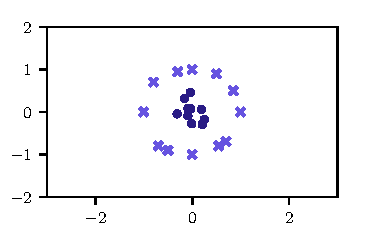
\includegraphics{non-sep-classes}
    \caption{Data set without any basis functions applied, not linearly separable.}
    \label{fig:non-sep-classes}
\end{figure}

It's obviously not possible for us to use a linear classifier to separate this two classes. However, if we apply a basis change by measuring the distance to the origin, we instead have \autoref{fig:basis-change-3d}, which is now linearly separable by a 2D plane between the two classes.
\begin{figure}[H]
    \centering
    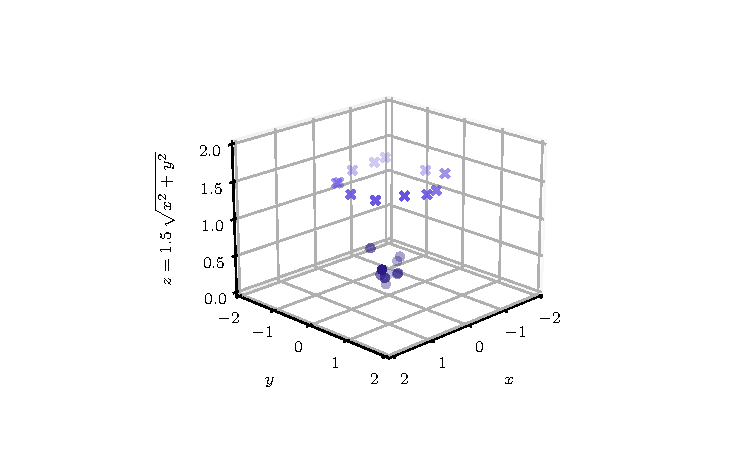
\includegraphics[width=0.5\paperwidth]{basis-change-3d}
    \caption{Data set with basis functions applied, now linearly separable.}
    \label{fig:basis-change-3d}
\end{figure}
Applying a generic basis change $\phi(\cdot)$, we can write our generalized linear model as:
\begin{equation}
		\label{eq:basis-changed-linear-model}
    h_k(\mathbf{x}, \mathbf{w}_k) = \mathbf{w}_k^\top \phi(\mathbf{x}) = \mathbf{w}_k^\top \mathbf{\phi}
\end{equation}
For the sake of simplicity in the rest of this chapter, we will leave out any basis changes in our derivations, but you should recognize that they could be applied to any of our input data to make the problems more tractable.

\begin{warning}
	For an input matrix $\mathbf{X}$, there is a matrix generalization of our basis transformed inputs: $\mathbf\Phi = \phi(\mathbf{X})$, where $\mathbf\Phi$ is known as the \textbf{design matrix}.
\end{warning}

\section{Numerical Parameter Optimization and Gradient Descent}
Recall from the previous chapter on linear regression that when it comes to optimizing our model's weight parameters $\mathbf{w}$, the goal is to minimize our loss function $\mathcal{L}(\mathbf{w})$. We did this by taking the derivative of our objective function with respect to $\mathbf{w}$, setting that expression equal to 0, and solving for $\mathbf{w}$. We were previously able to perform that procedure with confidence because the least squares loss function was \textit{strongly convex} with respect to the weight parameters, which meant it had a global solution we could solve for directly. Thus, the point of minimization for the objective function would occur where $\nabla \mathcal{L}(\mathbf{w}) = 0$.

Unfortunately, it's rarely the case that our objective function will be convex. In fact, in the next section, we will consider an objective function that is not convex, and as a result we will need a new way to optimize our parameters. Typically, when facing a non-convex objective function, we will need to resort to a \textit{numerical} procedure.

\begin{warning}
	The terms \textit{numerical} and \textit{analytical} procedures come up very frequently in machine learning literature. An analytical solution typically utilizes a closed form equation that accepts your model and input data and returns a solution in the form of optimized model parameters. On the other hand, numerical solutions are those that require some sort of iteration to move toward an ever better solution, eventually stopping once the solution is deemed `good enough'. Analytical solutions are typically more desirable than numerical solutions due to computational efficiency and performance guarantees, but they often are not possible for complex problems due to non-convexity.
\end{warning}

Gradient descent is one such numerical optimization technique.

\subsection{Gradient descent}
\begin{definition}[gradient descent]
	Gradient descent is a numerical, iterative optimization technique for finding the minimum of a function. It is often used to fit complex model parameters.
\end{definition}

The high level idea behind gradient descent is as follows: to update our parameters, we take a small step in the opposite direction of the gradient of our objective function with respect to the weight parameters $\mathbf{w}$. Notationally, this looks like the following:
\begin{equation}
	\label{eq:gradient-descent}
  \textbf{w}^{(t+1)} = \textbf{w}^{(t)} - \eta \nabla \mathcal{L}(\mathbf{w}^{(t)})
\end{equation}
where $\textbf{w}^{(t)}$ corresponds to the state of the parameters at time $t$, $\mathcal{L}(\textbf{w}^{(t)})$ is the gradient of our objective function, and $\eta > 0$ is known as the \textbf{learning rate}. Note that the parameter values at time $t = 0$ given by $\mathbf{w}^{(0)}$ are often initialized randomly.

\begin{warning}
	In general, we want a learning rate that is large enough so that we make progress toward reaching a better solution, but not so large that we take a step that puts us in a worse place in the parameter space than we were at the previous step. Notice in \autoref{fig:gradient-descent-step-size} that an appropriately small step size improves our objective function, while a large step size overshoots the update and leaves us in a worse position.
\end{warning}

\begin{figure}
    \centering
    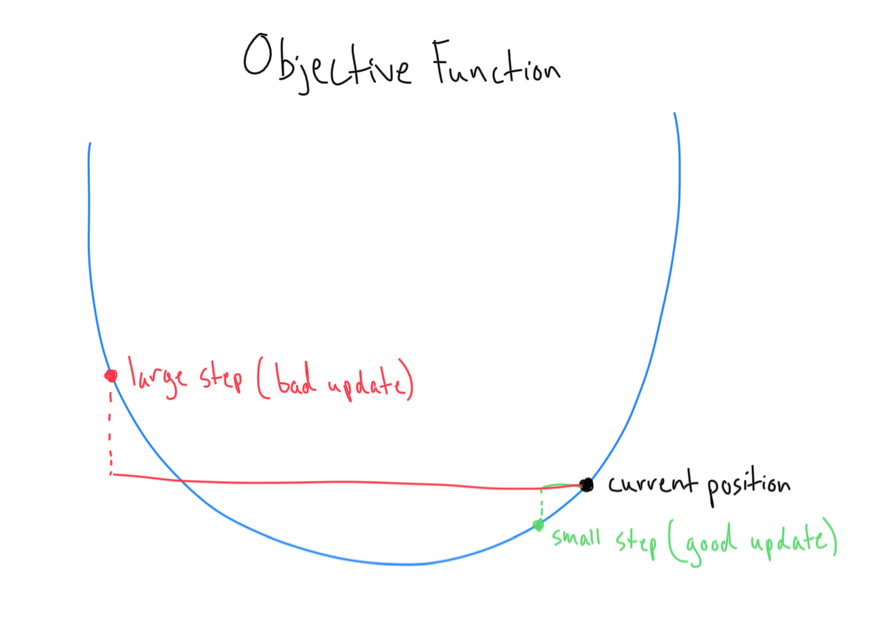
\includegraphics[width=0.5\paperwidth]{old/objective-function-classification.png}
    \caption{Step Size in Gradient Descent.}
    \label{fig:gradient-descent-step-size}
\end{figure}

Why take a step in the opposite direction of the gradient of the objective function? You can think of the objective function as a hill, and the current state of our parameters $\mathbf{w}^{(t)}$ is our position on that hill. The gradient tells us the steepest direction of increase in the objective function (i.e. it specifies the direction that will make our model worse). Since we want to minimize the objective function, we choose to move away from the direction of the gradient, sending our model down the hill towards an area of lower error. We typically cease optimization when our updates become sufficiently small, indicating that we've reached a local minimum. Note that it's a good idea to run gradient descent multiple times to settle on a final value for $\mathbf{w}$, ideally initializing $\mathbf{w}^{(0)}$ to a different starting value each time, because we are optimizing a function with multiple local minima.

\subsection{Stochastic gradient descent}
There are different means by which we can compute the gradient of our objective function at each step. The first way computes the gradient for our objective function at each step using the entire data set. In contrast, the technique known as \textbf{stochastic gradient descent} (also known as SGD) utilizes a subset (or \textit{batch}) of the data points at each step to compute the gradient, sometimes just a single data point. Stochastic gradient descent is typically a more popular technique for several reasons. First, the computation time is often significantly smaller as you don't need to pass over the entire data set at each iteration. Furthermore, it's less likely that you will get stuck in local minima while running SGD because a point in the parameter space that is a local minima for the entire data set combined is much less likely to be a local minima for each data point individually. Finally, SGD lends itself to being used for training online models (meaning models built on data points that are arriving at regular intervals) as the entirety of the data does not need to be present in order to train.

\section{Objectives for Decision Boundaries}
Now that we have a high-level understanding of what we're trying to accomplish with discriminant functions as well as a grasp on gradient descent, we can consider how to solve for the decision boundaries that will dictate our classification decisions. Similar to linear regression, we first need to establish an objective function to optimize. We begin with a very simple objective function known as \textbf{0/1 loss}.

\subsection{0/1 loss}
Recall that a loss function penalizes mistakes made by our model. The idea behind the \textbf{0/1 loss} function is very simple: if our model misclassifies a point, we incur a loss of 1, and if our model classifies it correctly, we incur no loss.

While this is a very intuitive loss function, it does not have a closed form solution like least squares does, and it is non-convex so it is not easily optimized. Intuitively, because we incur a loss of 0 or 1 for every prediction, we have no sense of `how good' a given prediction was. For example, one prediction could be very close to correct, while another could be way off, but they would both receive an equivalent loss of 1. Formally, because this loss function is not differentiable, we cannot get gradient information with which to optimize our model parameters $\mathbf{w}$. We will find a way around this in a moment when we discuss \textbf{hinge loss}, but before we get to that, let's consider using least squares loss as we did for linear regression.

\subsection{Least squares loss}
We are already familiar with the least squares loss function from linear regression, and we can apply it again in this context to find the set of weights $\mathbf{w}$ that form the optimal decision boundary between target classes.

We first need to introduce the idea of \textbf{one-hot encoding}, a method that allows us to represent each of our $K$ classes as vectors in $\mathbb{R}^K$. The idea is to map each class label $C_k$ and to the vector containing a 1 in its $k$-th entry and 0s everywhere else (note that classes usually are not 0-indexed). For example, if $K=4$, then class $C_2$ would be represented by the vector $[0, 1, 0, 0]^\top$. Now that we have the idea of one-hot encoding, we can describe our target classes for each data point in terms of a one-hot encoded vector, which can then be used in our training process for least squares.

Each class $C_k$ gets its own linear function with a different set of weights $\mathbf{w}_k$: $$h_k(\mathbf{x}, \mathbf{w}_k) = \mathbf{w}_k^\top \mathbf{x}.$$ We can combine the set of weights for each class into a matrix $\mathbf{W}$, which gives us our linear classifier: $$h(\mathbf{x}, \mathbf{W}) = \mathbf{W}^\top \mathbf{x}$$ where each row in the transposed weight matrix $\mathbf{W}^\top$ corresponds to the linear function of an individual class, and $\mathbf{W} \in \mathbb{R}^{D\times K}$. We can use the results derived in the last chapter to find the solution for $\mathbf{W}$ that minimizes the least squares loss function. Assuming a data set of input data points $\mathbf{X}$ and one-hot encoded target vectors $\mathbf{Y}$ (where every row is a single target vector, so that $\mathbf{Y}$ is $N\times K$), the optimal solution for $\mathbf{W}$ is given by: $$\mathbf{W}^{*} = (\mathbf{X}^\top\mathbf{X})^{-1}\mathbf{X}^\top\mathbf{Y},$$ which we can then use in our discriminant function $h(\mathbf{x}, \mathbf{W}^{*})$ to make predictions on new data points.

While least squares gives us an analytic solution for our discriminant function, it has significant limitations when used for classification. For one, least squares penalizes data points that are `too good', meaning they fall too far on the correct side of the decision boundary. Furthermore, it is not robust to outliers, meaning the decision boundary significantly changes with the addition of just a few outlier data points, as seen in \autoref{fig:outliers}.

\begin{figure}
    \centering
    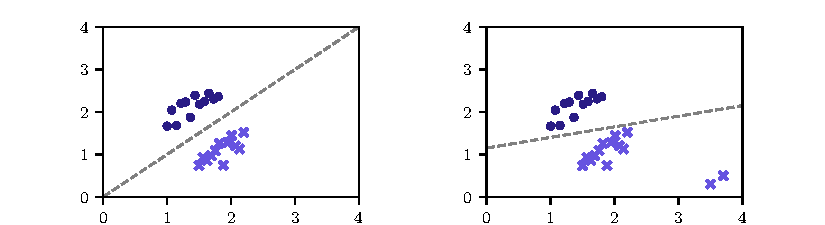
\includegraphics{outliers}
    \caption{Outliers significantly impact our decision boundary.}
    \label{fig:outliers}
\end{figure}

We can help remedy the problems with least squares by using an alternative loss function for determining our weight parameters.

\subsection{Hinge loss}
Recall that the problem with 0/1 loss was that we couldn't use it optimize our model parameters $\mathbf{w}$. It didn't produce a closed form solution like least squares loss, and it wasn't differentiable so we couldn't take gradients.

The hinge loss function is a modification of the 0/1 loss function that both provides more fine-grained information about the `goodness' of a prediction and makes the loss function differentiable. To understand the hinge loss function, it's first necessary to introduce the \textbf{rectified linear activation unit}, known as ReLU, seen in \autoref{fig:relu-fn}: $$\operatorname{ReLU}(z) = \max\{0, z\}.$$ We can use the form of this function to our advantage in constructing the hinge loss by recognizing that we wish to incur error when we're wrong (which corresponds to $z > 0$, the right side of the graph that is continuously increasing), and we wish to incur 0 error if we are correct (which corresponds to the left side of the graph where $z < 0$).
\begin{figure}
    \centering
    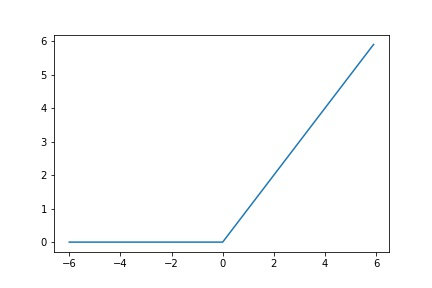
\includegraphics[width=0.5\paperwidth]{old/relu_fn_GEN.jpg}
    \caption{Form of the ReLU function.}
    \label{fig:relu-fn}
\end{figure}

Remember from the previous section on least squares that in the two-class case, we classify a data point $\textbf{x}^{*}$ as being from class 1 if $h(\mathbf{x}, \mathbf{w}) \geq 0$, and class -1 otherwise. We can combine this logic with ReLU by recognizing that $-h(\textbf{x}^{*}, \textbf{w})y^{*} \geq 0$ when there is a classification error, where $y^{*}$ is the true class of data point $\mathbf{x}$. This has exactly the properties we described above: we incur error when we misclassify, and otherwise we do not incur error.

We can then write the entirety of the hinge loss function:
\begin{align}
	\mathcal{L}(\textbf{w}) &= \sum_{i=1}^{N} \text{ReLU}(-h(\textbf{x}_{i}, \textbf{w})y_{i}) \\
	&= -\sum_{y_{i} \neq \hat{y}_{i}}^{N} h(\textbf{x}_{i}, \textbf{w})y_{i} \\
	&= -\sum_{y_{i} \neq \hat{y}_{i}}^{N} \textbf{w}^\top\textbf{x}_{i} y_{i}
\end{align}
where $\hat{y}_{i}$ is our class prediction and $y_{i}$ is the true class value. Notice that misclassified examples contribute positive loss, as desired. We can take the gradient of this loss function, which will allow us to optimize it using stochastic gradient descent. The gradient of the loss with respect to our parameters \textbf{w} is as follows:
\begin{align*}
	\frac{\partial \mathcal{L}(\textbf{w})}{\partial \textbf{w}} = -\sum_{y_{i} \neq \hat{y}_{i}}^{N} \textbf{x}_{i} y_{i}
\end{align*}
and then our update equation from time $t$ to time $t+1$ for a single misclassified example and with learning rate $\eta$ is given by:
\begin{align*}
	\textbf{w}^{(t+1)} = \textbf{w}^{(t)} - \eta\frac{\partial \mathcal{L}(\textbf{w})}{\partial \textbf{w}} = \textbf{w}^{(t)} + \eta \textbf{x}_{i} y_{i}
\end{align*}

To sum up, the benefits of the hinge loss function are its differentiability (which allows us to optimize our weight parameters), the fact that it doesn't penalize any correctly classified data points (unlike basic linear classification), and that it penalizes more heavily data points that are more poorly misclassified.

Using hinge loss with discriminant functions to solve classification tasks (and applying stochastic gradient descent to optimize the model parameters) is known as the \textbf{perceptron algorithm}. The perceptron algorithm guarantees that if there is separability between all of our data points and we run the algorithm for long enough, we will find a setting of parameters that perfectly separates our data set. The proof for this is beyond the scope of this textbook.

\section{Probabilistic Methods}
Unsurprisingly, we can also cast the problem of classification into a probabilistic context, which we now turn our attention to. Within this setting, we have a secondary choice to make between two distinct probabilistic approaches: discriminative or generative. We will explore both of these options.

\subsection{Probabilistic Discriminative Models}
Ultimately, our classification task can be summarized as follows: \textit{given a new data point $\textbf{x}^{*}$, can we accurately predict the target class $y^{*}$?}

Given this problem statement, it makes sense that we might try to model $p(y^*|\textbf{x}^*)$. In fact, modeling this conditional distribution directly is what's known as \textbf{probabilistic discriminative modeling}.

\begin{definition}[probabilistic discriminative modeling]
    Probabilistic modeling is a classification technique whereby we choose to directly model the conditional class distribution in order to make classification predictions.
\end{definition}

This means that we will start with the functional form of the generalized linear model described by Equation \ref{basis-changed-linear-model}, convert this to a conditional distribution, and then optimize the parameters of the conditional distribution directly using a maximum likelihood procedure. From here, we will be able to make predictions on new data points $\textbf{x}^{*}$. The key feature of this procedure, which is known as \textit{discriminative training}, is that it optimizes the parameters of a conditional distribution directly. We describe a specific, common example of this type of procedure called \textbf{logistic regression} in the next section.

\subsubsection{Logistic Regression}
One problem we need to face in our discriminative modeling paradigm is that the results of our generalized linear model are not probabilities; they are simply real numbers. This is why in the previous paragraph we mentioned needing to convert our generalized linear model to a conditional distribution. That step boils down to somehow squashing the outputs of our generalized linear model onto the real numbers between 0 and 1, which will then correspond to probabilities. To do this, we will apply what is known as the \textbf{logistic sigmoid function}, $\sigma(\cdot)$.

\begin{definition}[logistic sigmoid function, $\sigma(\cdot)$]
	The logistic sigmoid function is commonly used to compress the real number line down to values between 0 and 1. It is defined functionally as:
	\begin{align*}
		\sigma(z) = \frac{1}{1 + \exp{(-z)}}
	\end{align*}
	As you can see in Figure \ref{fig:log-sig-fn} where the logistic sigmoid function is graphed, it squashes our output domain between 0 and 1 as desired for a probability.
\end{definition}

\begin{figure}
    \centering
    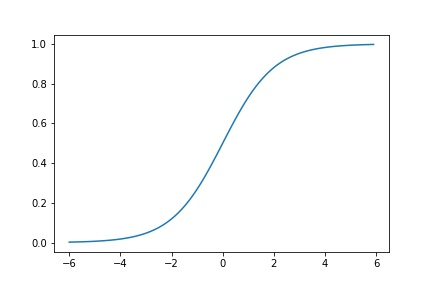
\includegraphics[width=0.5\paperwidth]{old/log_sig_fn_GEN.jpg}
    \caption{Logistic Sigmoid Function.}
    \label{fig:log-sig-fn}
\end{figure}

\begin{warning}
    There is a more satisfying derivation for our use of the logistic sigmoid function in logistic regression, but understanding its squashing properties as motivation is sufficient for the purposes of this book.
\end{warning}

Using the logistic sigmoid function, we now have a means of generating a probability that a new data point $\textbf{x}^{*}$ is part of class $y^{*}$. Because we are currently operating in the two-class case, which in this context will be denoted $C_{1}$ and $C_{2}$, we'll write the probability for each of these classes as:
\begin{align*}
	p(y^{*}=C_{1}|\textbf{x}^{*}) &= \sigma(\textbf{w}^\top\textbf{x}^{*}) \\
	p(y^{*}=C_{2}|\textbf{x}^{*}) &= 1 - p(y^{*}=C_{1}|\textbf{x}^{*})
\end{align*}
Now that we have such functions, we can apply the maximum likelihood procedure to determine the optimal parameters for our logistic regression model.

For a data set \{$\textbf{x}_{i}, y_{i}$\} where $i = 1..N$ and $y_{i} \in \{0,1\}$, the likelihood for our setting of parameters $\textbf{w}$ can be written as:
\begin{equation} \label{log-reg-likelihood}
	p(\{y_{i}\}_{i=1}^{N}|\textbf{w}) = \prod_{i=1}^{N} \hat{y}_{i}^{y_{i}} \{1 - \hat{y}_{i}\}^{1 - y_{i}}
\end{equation}
where $\hat{y}_{i} = p(y_{i}=C_{1}|\textbf{x}_{i}) = \sigma(\textbf{w}^\top\textbf{x}_{i})$.

In general, we would like to maximize this probability to find the optimal setting of our parameters. This is exactly what we intend to do, but with two further simplifications. First, we're going to maximize the probability of the \textit{logarithm} of the likelihood, as in Equation \ref{take-log-of-probability}.

\begin{equation} \label{take-log-of-probability}
    \ln(p(\{y_{i}\}_{i=1}^{N}|\textbf{w})) = \sum_{i=1}^{N} \{y_{i}\ln{\hat{y}_i} + (1 - y_{i})\ln{(1-\hat{y_{i}})}\}
\end{equation}

As a monotonically increasing function, maximizing the logarithm of the likelihood (called the \textit{log likelihood}) will result in the same optimal setting of parameters as if we had just optimized the likelihood directly. Furthermore, using the log likelihood has the nice effect of turning what is currently a product of terms from $1..N$ to a sum of terms from $1..N$, which will make our calculations nicer.

Second, we will turn our log likelihood into an \textit{error function} by taking the negative of our log likelihood expression. Now, instead of maximizing the log likelihood, we will be minimizing the error function, which will again find us the same setting of parameters.

\begin{warning}
    It's worth rereading the above paragraph again to understand the pattern presented there, which we will see several times throughout this book. Instead of maximizing a likelihood function directly, it is often easier to define an error function using the negative log likelihood, which we can then minimize to find the optimal setting of parameters for our model.
\end{warning}

After taking the negative logarithm of the likelihood function defined by Equation \ref{log-reg-likelihood}, we are left with the following term, known as the \textit{cross-entropy error function}, which we will seek to minimize:
\begin{equation} \label{cross-entropy-error-fn}
	\mathrm{E}(\textbf{w}) = - \ln{p(\{y_{i}\}|\textbf{w})} = - \sum_{i=1}^{N} \{y_{i}\ln{\hat{y}_i} + (1 - y_{i})\ln{(1-\hat{y_{i}})}\}
\end{equation}
where as before $\hat{y}_{i} = p(y_{i}=C_{1}|\textbf{x}_{i}) = \sigma(\textbf{w}^\top\textbf{x}_{i})$.
The cross-entropy error refers to the  log likelhood of the labels conditioned on the examples. When used with the specific form of the logistic regression, this is also the {\em logistic loss}. 
Now, to solve for the optimal setting of parameters using a maximum likelihood approach as we've done previously, we start by taking the gradient of the cross-entropy error function with respect to \textbf{w}:
\begin{equation} \label{log-reg-gradient}
	\nabla \mathrm{E}(\textbf{w}) = \sum_{i=1}^{N}(\hat{y}_{i} - y_{i})\textbf{x}_{i}
\end{equation}
which we arrive at by recognizing that the derivative of the logistic sigmoid function can be written in terms of itself as:
\begin{align*}
	\frac{\partial \sigma(z)}{\partial z} = \sigma(z)(1 - \sigma(z))
\end{align*}
Let's inspect the form of Equation \ref{log-reg-gradient} for a moment to understand its implications. First, it's a summation over all of our data points, as we would expect. Then, for each data point, we are taking the difference between our predicted value $\hat{y}_{i}$ and the actual value $y_{i}$, and multiplying that difference by the input vector $\textbf{x}_{i}$.

While a closed form solution does not present itself here as it did in the case of linear regression due to the nonlinearity of the logistic sigmoid function, we can still optimize the parameters \textbf{w} of our model using an iterative procedure like gradient descent, where the objective function is defined by Equation \ref{cross-entropy-error-fn}.

\subsubsection{Multi-Class Logistic Regression and Softmax}
As we saw when working with discriminant functions, we also need to account for multi-class problems, which are practically speaking more common than the simple two-class scenario.

In the logistic regression setting (which is a form of \textit{discriminative modeling}, not to be confused with \textit{discriminant functions}), we are now working with probabilities, which is why we introduced the `probability squashing' sigmoidal function $\sigma(\cdot)$. Note that the sigmoidal function is also sometimes known as the sigmoidal activation function.

Similarly, in the multi-class logistic regression setting, we would like to also have a probability squashing function that generalizes beyond two classes. This generalization of the sigmoidal function is known as \textbf{softmax}.

\begin{definition}[softmax]
Softmax is the multi-class generalization of the sigmoidal activation function. It accepts a vector of activations (inputs) and returns a vector of probabilities corresponding to those activations. It is defined as follows:
\begin{align*}
	\text{softmax}_{k}(\textbf{z}) = \frac{\exp{(z_{k})}}{\sum_{i=1}^{K} \exp{(z_{i})}}\text{, for all $k$}
\end{align*}
\end{definition}

Multi-class logistic regression uses softmax over a vector of activations to select the most likely target class for a new data point. It does this by applying softmax and then assigning the new data point to the class with the highest probability.

\begin{example}{Softmax Example}{softmax-example}
	Consider an example that has three classes: $C_{1}, C_{2}, C_{3}$. Let's say we have an activation vector \textbf{z} for our new data point $\textbf{x}$ that we wish to classify, given by:
	\begin{align*}
		\textbf{z} = \textbf{W}^\top\textbf{x} =
			\begin{bmatrix}
		    	4 \\
		        1 \\
		        7
		    \end{bmatrix}
	\end{align*}
	where
	\begin{align*}
		\textbf{z}_{j} = \textbf{w}_{j}^\top\textbf{x}
	\end{align*}
	Then, using our definition of softmax, we have:
	\begin{align*}
		\text{softmax}(\textbf{z}) =
			\begin{bmatrix}
				0.047 \\
				0.002 \\
				0.950
		    \end{bmatrix}
	\end{align*}
	And therefore, we would assign our new data point $\textbf{x}$ to class $C_{3}$, which has the largest activation.
\end{example}

As in the two-class logistic regression case, we now need to solve for the parameters \textbf{W} of our model, also written as \{$\textbf{w}_{j}$\}. Assume we have an observed data set \{$\textbf{x}_{i}, \textbf{y}_{i}$\} for $i=1..N$ where $\textbf{y}_{i}$ are one-hot encoded target vectors.  We begin this process by writing the likelihood for our data, which is only slightly modified here to account for multiple classes:

\begin{equation} \label{multi-class-log-reg-likelihood}
	p(\{\textbf{y}_{i}\}_{i=1}^{N}|\textbf{W}) = \prod_{i=1}^{N}\prod_{j=1}^{K} p(\textbf{y}_{i}=C_{j}|\textbf{x}_{i})^{y_{ij}} = \prod_{i=1}^{N}\prod_{j=1}^{K} \hat{y}_{ij}^{y_{ij}}
\end{equation}
where $\hat{y}_{ij} = \text{softmax}_{j}(\textbf{W}\textbf{x}_{i})$ \newline

We can now take the negative logarithm to get the cross-entropy error function for the multi-class classification problem:
\begin{equation} \label{multi-class-cross-entropy-error-fn}
	\mathrm{E}(\textbf{W}) = - \ln{p(\{\textbf{y}_{i}\}_{i=1}^{N}|\textbf{W})} = - \sum_{i=1}^{N}\sum_{j=1}^{K} y_{ij} \ln{\hat{y}_{ij}}
\end{equation}
As in the two-class case, we now take the gradient with respect to one of our weight parameter vectors $\textbf{w}_{j}$:
\begin{equation} \label{multi-class-log-reg-gradient}
	\nabla_{\textbf{w}_{j}} \mathrm{E}(\textbf{W}) = \sum_{i=1}^{N}(\hat{y}_{ij} - y_{ij})\textbf{x}_{i}
\end{equation}
which we arrived at by recognizing that the derivative of the softmax function with respect to the input activations $z_{j}$ can be written in terms of itself:
\begin{align*}
	\frac{\partial \text{softmax}_{k}(z)}{\partial z_{j}} = \text{softmax}_{k}(z)(\mathrm{I}_{kj} - \text{softmax}_{j}(z))
\end{align*}
where $\mathrm{I}$ is the identity matrix.

As in the two-class case, now that we have this gradient expression, we can use an iterative procedure like gradient descent to optimize our parameters $\textbf{W}$.

\subsection{Probabilistic Generative Models}
With the probabilistic discriminative modeling approach, we elected to directly model $p(y^{*}|\textbf{x}^{*})$. However, there was an alternative option: we could have instead modeled the joint distribution of the class $y^{*}$ and the input data point $\textbf{x}^{*}$ together as $p(y^{*}, \textbf{x}^{*})$. This approach is what's known as \textbf{probabilistic generative modeling} because we actually model the process by which the data was generated.

To model the data generating process in classification tasks generally acknowledges that a data point is produced by first selecting a class $y^{*}$ from a categorical class prior $p(y^{*})$ and then generating the data point $\textbf{x}^{*}$ itself from the class-conditional distribution $p(\textbf{x}^{*}|y^{*})$, the form of which is problem specific. This generative approach is a particularly good idea if we want to create more data (by sampling from the joint distribution) or if we have some sort of expert knowledge about how the data was generated, which can make our model more powerful than the discriminative approach.

\begin{warning}
    Notice that with probabilistic generative modeling, we choose a specific distribution for our class-conditional densities instead of simply using a generalized linear model combined with a sigmoid/softmax function as we did in the logistic regression setting. This highlights the difference between discriminative and generative modeling: in the generative setting, we are modeling the production of the data itself instead of simply optimizing the parameters of a more general model that predicts class membership directly.
\end{warning}

\subsubsection{Classification in the Generative Setting}
Now that we're situated in the generative setting, we turn our attention to the actual problem of using our model to predict class membership of new data points $\textbf{x}^{*}$.

To perform classification, we will pick the class $C_{k}$ that maximizes the probability of $\textbf{x}^{*}$ being from that class as defined by $p(y^{*} = C_{k} | \textbf{x}^{*})$. We can relate this conditional density to the joint density $p(y^{*}, \textbf{x}^{*})$ through Bayes' Rule:
\begin{align*}
	p(y^{*} = C_{k} | \textbf{x}^{*}) = \frac{p(y^{*}, \textbf{x}^{*})}{p(\textbf{x}^{*})} = \frac{p(\textbf{x}^{*} | y^{*} = C_{k})p(y^{*} = C_{k})}{p(\textbf{x}^{*})} \propto p(\textbf{x}^{*} | y^{*} = C_{k})p(y^{*} = C_{k})
\end{align*}
where $p(\textbf{x}^{*})$ is a constant that can be ignored as it will be the same for every conditional probability $p(y^{*} = C_{k}|\textbf{x}^{*})$.

Recall that the class prior $p(y)$ will always be a categorical distribution (the multi-class generalization of the Bernoulli distribution), while the class-conditional distribution can be specified using prior knowledge of the problem domain. Once we have specified this class conditional distribution, we can solve for the parameters of both that model and the categorical distribution by optimizing the likelihood function. Let's now derive that likelihood function.

\begin{derivation}[probabilistic generative model likelihood function]

    We're going to derive the likelihood function for the parameters of our probabilistic generative model in the two-class setting, allowing that the multi-class generalization will be a straightforward exercise.

    Let's start by assuming a Gaussian conditional distribution for our data $p(\textbf{x} | y = C_{k})$. Given a data set \{$\textbf{x}_{i}, y_{i}$\} for $i = 1..N$, where $y_{i} = 1$ corresponds to class $C_{1}$ and $y_{i} = 0$ corresponds to class $C_{2}$, we can construct our maximum likelihood solution. Let's first specify our class priors:
    \begin{align*}
    	p(C_{1}) &= \pi \\
    	p(C_{2}) &= 1 - \pi
    \end{align*}
    For simplicity, we'll assume a shared covariance matrix $\boldsymbol{\Sigma}$ between our two classes. Then, for data points $\textbf{x}_{i}$ from class $C_{1}$, we have:
    \begin{align*}
    	p(\textbf{x}_{i}, C_{1}) = p(C_{1})p(\textbf{x}_{i}|C_{1}) = \pi\mathcal{N}(\textbf{x}_{i} | \boldsymbol{\mu}_{1}, \boldsymbol{\Sigma})
    \end{align*}
    And for data points $\textbf{x}_{i}$ from class $C_{2}$, we have:
    \begin{align*}
    	p(\textbf{x}_{i}, C_{2}) = p(C_{2})p(\textbf{x}_{i}|C_{2}) = (1-\pi)\mathcal{N}(\textbf{x}_{i} | \boldsymbol{\mu}_{2}, \boldsymbol{\Sigma})
    \end{align*}
    Using these two densities, we can construct our likelihood function:
    \begin{align*}
    	p(\pi, \boldsymbol{\mu}_{1}, \boldsymbol{\mu}_{2}, \boldsymbol{\Sigma}) = \prod_{i=1}^{N} \bigg( \pi\mathcal{N}(\textbf{x}_{i} | \boldsymbol{\mu}_{1}, \boldsymbol{\Sigma}) \bigg)^{y_{i}} \bigg( (1-\pi)\mathcal{N}(\textbf{x}_{i} | \boldsymbol{\mu}_{2}, \boldsymbol{\Sigma}) \bigg)^{1 - y_{i}}
    \end{align*}
    As usual, we will take the logarithm which is easier to work with:
    \begin{align*}
    	\ln p(\pi, \boldsymbol{\mu}_{1}, \boldsymbol{\mu}_{2}, \boldsymbol{\Sigma}) = \sum_{i=1}^{N} y_{i} \ln \bigg( \pi\mathcal{N}(\textbf{x}_{i} | \boldsymbol{\mu}_{1}, \boldsymbol{\Sigma}) \bigg) + (1 - y_{i}) \ln \bigg( (1-\pi)\mathcal{N}(\textbf{x}_{i} | \boldsymbol{\mu}_{2}, \boldsymbol{\Sigma}) \bigg)
    \end{align*}
\end{derivation}
Now that we have specified the log-likelihood function for our model, we can go about optimizing our model by maximizing this likelihood. One way to do this is with a straightforward maximimum likelihood estimation approach. We will optimize our parameters $\pi, \boldsymbol{\mu}_{1}, \boldsymbol{\mu}_{2}, \text{and}, \boldsymbol{\Sigma}$ separately, using the usual procedure of taking the derivative, setting equal to 0, and then solving for the parameter of interest. We write down this MLE solution in the following section.

\subsubsection{MLE Solution}

\textbf{Solving for $\boldsymbol{\pi}$} \newline
Beginning with $\pi$, we'll concern ourselves only with the terms that depend on $\pi$ which are:
\begin{align*}
	\sum_{i=1}^{N} y_{i}\ln{\pi} + (1-y_{i})\ln{(1 - \pi)}
\end{align*}
Taking the derivative with respect to $\pi$, setting equal to 0, rearranging, we get:
\begin{align*}
	\pi = \frac{1}{N} \sum_{i=1}^{N} y_{i} = \frac{N_{1}}{N} = \frac{N_{1}}{N_{1} + N_{2}}
\end{align*}
where $N_{1}$ is the number of data points in our data set from class $C_{1}$, $N_{2}$ is the number of data points from class $C_{2}$, and $N$ is just the total number of data points. This means that the maximum likelihood solution for $\pi$ is the fraction of points that are assigned to class $C_{1}$, a fairly intuitive solution and one that will be commonly seen when working with maximum likelihood calculations. \newline \newline
\textbf{Solving for $\boldsymbol{\mu}$} \newline
Let's now perform the maximization for $\boldsymbol{\mu}_{1}$. Start by considering the terms from our log likelihood involving $\boldsymbol{\mu}_{1}$:
\begin{align*}
	\sum_{i=1}^{N} y_{i} \ln \mathcal{N}(\textbf{x}_{i} | \boldsymbol{\mu}_{1}, \boldsymbol{\Sigma}) = -\frac{1}{2} \sum_{i=1}^{N} y_{i} (\textbf{x}_{i} - \boldsymbol{\mu}_{1})^\top\boldsymbol{\Sigma}^{-1}(\textbf{x}_{i} - \boldsymbol{\mu}_{1}) + c
\end{align*}
where $c$ are constants not involving the $\boldsymbol{\mu}_{1}$ term. Taking the derivative with respect to $\boldsymbol{\mu}_{1}$, setting equal to 0, and rearranging:
\begin{align*}
	\boldsymbol{\mu}_{1} = \frac{1}{N_{1}} \sum_{i=1}^{N} y_{i}\textbf{x}_{i}
\end{align*}
which is simply the average of all the data points $\textbf{x}_{i}$ assigned to class $C_{1}$, a very intuitive result. By the same derivation, the maximum likelihood solution for $\boldsymbol{\mu}_{2}$ is:
\begin{align*}
	\boldsymbol{\mu}_{2} = \frac{1}{N_{2}} \sum_{i=1}^{N} (1-y_{i})\textbf{x}_{i}
\end{align*}
\textbf{Solving for $\boldsymbol{\Sigma}$} \newline

We can also the maximum likelihood solution for the shared covariance matrix $\boldsymbol{\Sigma}$. Start by considering the terms in our log likelihood expression involving $\boldsymbol{\Sigma}$:
\begin{align*}
  -\frac{1}{2} \sum_{i=1}^{N} y_{i} \ln{|\boldsymbol{\Sigma}|} &-\frac{1}{2} \sum_{i=1}^{N} y_{i} (\textbf{x}_{i} - \boldsymbol{\mu}_{1})^\top\boldsymbol{\Sigma}^{-1}(\textbf{x}_{i} - \boldsymbol{\mu}_{1}) -\frac{1}{2} \sum_{i=1}^{N} (1-y_{i}) \ln{|\boldsymbol{\Sigma}|} 
  \\
  & -\frac{1}{2} \sum_{i=1}^{N} (1-y_{i}) (\textbf{x}_{i} - \boldsymbol{\mu}_{2})^\top\boldsymbol{\Sigma}^{-1}(\textbf{x}_{i} - \boldsymbol{\mu}_{2})
\end{align*}


We can use the following ``matrix cookbook formulas'' to help with taking  the derivative with respect to $\boldsymbol{\Sigma}$.
Also, we adopt convention 
${\mathbf Z}^{-\top} := (\mathbf{Z}^{\top})^{-1}$.
%
The two helpful formulas are:
\begin{align*}
  & \frac{\partial \mathbf{a}^\top \mathbf{Z}^{-1} \mathbf{b}}{\partial \mathbf{Z}} = - \mathbf{Z}^{-\top} \mathbf{a} \mathbf{b}^\top \mathbf{Z}^{-\top} \\
  & \frac{\partial \ln | \det (\mathbf{Z}) |}{\partial \mathbf{Z}} = \mathbf{Z}^{-\top}.
 \end{align*}

 Now, taking the derivative with respect to $\boldsymbol{\Sigma}$ and collecting terms, we have:
\begin{align*}
\frac{1}{2}	N\boldsymbol{\Sigma}^{-\top} - \frac{1}{2}\sum_{i=1}^{N} y_{i} \boldsymbol{\Sigma}^{-\top}(\textbf{x}_{i} - \boldsymbol{\mu}_{1})(\textbf{x}_{i} - \boldsymbol{\mu}_{1})^\top\boldsymbol{\Sigma}^{-\top} - \frac{1}{2}\sum_{i=1}^{N} (1-y_{i}) \boldsymbol{\Sigma}^{-\top}(\textbf{x}_{i} - \boldsymbol{\mu}_{2})(\textbf{x}_{i} - \boldsymbol{\mu}_{2})^\top\boldsymbol{\Sigma}^{-\top}
\end{align*}

Setting this to zero and multiplying both sides by $\boldsymbol{\Sigma}^\top$
from the left and right (with the effect of retaining $\boldsymbol{\Sigma}^\top$ in only the first term, since $\boldsymbol{\Sigma}^\top \boldsymbol{\Sigma}^{-\top}=\boldsymbol{\Sigma}^\top\left(\boldsymbol{\Sigma}^\top\right)^{-1}=\mathbf{I}$ and $\boldsymbol{\Sigma}^{-\top} \boldsymbol{\Sigma}^{\top}=\left(\boldsymbol{\Sigma}^\top\right)^{-1}\boldsymbol{\Sigma}^{\top}=\mathbf{I}$), and multiplying by 2, 
we have
\begin{align*}
N	\boldsymbol{\Sigma}^\top - \sum_{i=1}^{N} \bigg( y_{i}(\textbf{x}_{i} - \boldsymbol{\mu}_{1})(\textbf{x}_{i} - \boldsymbol{\mu}_{1})^\top + (1-y_{i})(\textbf{x}_{i} - \boldsymbol{\mu}_{2})(\textbf{x}_{i} - \boldsymbol{\mu}_{2})^\top \bigg) = 0.
\end{align*}

Rearranging to solve for $\boldsymbol{\Sigma}$, and recognizing that covariance matrices are symmetric, and so
$	\boldsymbol{\Sigma}^\top = 	\boldsymbol{\Sigma}$, 
we have:
%
\begin{align*}
	\boldsymbol{\Sigma} = \frac{1}{N} \sum_{i=1}^{N} \bigg( y_{i}(\textbf{x}_{i} - \boldsymbol{\mu}_{1})(\textbf{x}_{i} - \boldsymbol{\mu}_{1})^\top + (1-y_{i})(\textbf{x}_{i} - \boldsymbol{\mu}_{2})(\textbf{x}_{i} - \boldsymbol{\mu}_{2})^\top \bigg).
\end{align*}


This has the intuitive interpretation that the maximum likelihood solution for the shared covariance matrix is the weighted average of the two individual covariance matrices.
Note that $(\mathbf{x}_i - \boldsymbol{\mu}_1)(\mathbf{x}_i - \boldsymbol{\mu}_1)^\top$ is a matrix (the outer product of the two vectors). Also, $y_i$ is a scalar, which means that each term is a sum of matrices. For any point $i$, only one of two matrices inside will contribute due to the use  of $y_i$ and $(1-y_i)$.
\newline

It is relatively straightforward to extend these maximum likelihood derivations from their two-class form to their more general, multi-class form.
\if 0
%
%dcp commented out because in pset 2
%
If there are $K$ classes this expression becomes
%
$$\frac{1}{N} \sum_{i=1}^N \sum_{k=1}^K 1[y_i=k](\mathbf{x}_i - \boldsymbol{\mu}_k)(\mathbf{x}_i - \boldsymbol{\mu}_k)^\top  $$
%
(up to some constants) where $1[a=b]$ is $1$ if $a=b$ and $0$ otherwise.
\fi



\subsubsection{Naive Bayes}
There exists a further simplification to probabilistic generative modeling in the context of classification known as \textbf{Naive Bayes}.

\begin{definition}[naive Bayes]
	Naive Bayes is a type of generative model for classification tasks. It imposes the simplifying rule that for a given class $C_{k}$, we assume that each feature of the data points $\textbf{x}$ generated within that class are independent (hence the descriptor `naive'). This means that the conditional distribution $p(\textbf{x} | y = C_{k})$ can be written as:
	\begin{align*}
		p(\textbf{x} | y = C_{k}) = \prod_{i = 1}^{D} p(x_{j} | y = C_{k})
	\end{align*}
	where $D$ is the number of features in our data point $\textbf{x}$ and $C_{k}$ is the class. Note that Naive Bayes does not specify the form of the model $p(x_{j} | y = C_{k})$, this decision is left up to us.
\end{definition}
This is obviously not a realistic simplification for all scenarios, but it can make our calculations easier and may actually hold true in certain cases. We can build more intuition for how Naive Bayes works through an example.

\begin{example}{Naive Bayes Example}{naive-bayes-example}
	Suppose you are given a biased two-sided coin and two biased dice. The coin has probabilities as follows:
	\begin{align*}
		\textbf{Heads}: 30\% \\
		\textbf{Tails}: 70\%
	\end{align*}
	The dice have the numbers 1 through 6 on them, but they are biased differently. Die 1 has probabilities as follows:
	\begin{align*}
		\textbf{1}: 40\% \\
		\textbf{2}: 20\% \\
		\textbf{3}: 10\% \\
		\textbf{4}: 10\% \\
		\textbf{5}: 10\% \\
		\textbf{6}: 10\%
	\end{align*}
	Die 2 has probabilities as follows:
	\begin{align*}
		\textbf{1}: 20\% \\
		\textbf{2}: 20\% \\
		\textbf{3}: 10\% \\
		\textbf{4}: 30\% \\
		\textbf{5}: 10\% \\
		\textbf{6}: 10\%
	\end{align*}
	Your friend is tasked with doing the following. First, they flip the coin. If it lands Heads, they select Die 1, otherwise they select Die 2. Then, they roll that die 10 times in a row, recording the results of the die rolls. After they have completed this, you get to observe the aggregated results from the die rolls. Using this information (and assuming you know the biases associated with the coin and dice), you must then classify which die the rolls came from. Assume your friend went through this procedure and produced the following counts:
	\begin{align*}
		\textbf{1}: 3 \\
		\textbf{2}: 1 \\
		\textbf{3}: 2 \\
		\textbf{4}: 2 \\
		\textbf{5}: 1 \\
		\textbf{6}: 1
	\end{align*}
	Determine which die this roll count most likely came from. \newline \newline

	\textbf{Solution:} \newline
	This problem is situated in the Naive Bayes framework: for a given class (dictated by the coin flip), the outcomes within that class (each die roll) are independent. Making a classification in this situation is as simple as computing the probability that the selected die produced the given roll counts. Let's start by computing the probability for Die 1:
	\begin{align*}
		p(\text{Die 1}) &= p(\text{Coin Flip = Heads}) * p(\text{Roll Count = }[3,1,2,2,1,1]) \\
		&\propto 0.3 * (0.4)^{3} * (0.2)^{1} * (0.1)^{2} * (0.1)^{2} * (0.1)^{1} * (0.1)^{1} \\
		&\propto 3.84 * 10^{-9}
	\end{align*}
	Notice that we don't concern ourselves with the normalization constant for the probability of the roll count - this will not differ between the choice of dice and we can thus ignore it for simplicity. Now the probability for Die 2:
	\begin{align*}
		p(\text{Die 2}) &= p(\text{Coin Flip = Tails}) * p(\text{Roll Count = }[3,1,2,2,1,1]) \\
		&\propto 0.7 * (0.2)^{3} * (0.2)^{1} * (0.1)^{2} * (0.3)^{2} * (0.1)^{1} * (0.1)^{1} \\
		&\propto 1.008 * 10^{-8}
	\end{align*}
	Therefore, we would classify this roll count as having come from Die 2. \newline \newline
	Note that this problem asked us only to make a classification prediction after we already knew the parameters governing the coin flip and dice rolls. However, given a data set, we could have also used a maximum likelihood procedure under the Naive Bayes assumption to estimate the values of the parameters governing the probability of the coin flip and die rolls.
\end{example}

\section{Conclusion}
In this chapter, we looked at different objectives and techniques for solving classification problems, including discriminant functions, probabilistic discriminative models, and probabilistic generative models. In particular, we emphasized the distinction between two-class and multi-class problems as well as the philosophical differences between generative and discriminative modeling.

We also covered several topics that we will make use of in subsequent chapters, including sigmoid functions and softmax, maximum likelihood solutions, and further use of basis changes.

By now, you have a sound understanding of generative modeling and how it can be applied to classification tasks. In the next chapter, we will explore how generative modeling is applied to a still broader class of problems.

  % \chapter{Neural Networks}
Despite how seemingly popular neural networks have become recently, they aren't actually a novel technique. The first neural networks were described in the early 1940s, and the only reason they weren't put into practice shortly thereafter was the fact that we didn't yet have access to the large amounts of storage and compute that complex neural network require. Over the last two decades, and particularly with the advent of cloud computing, we now have more and more access to the cheap processing power and memory required to make neural networks a viable option for model building.

As we will come to see in this chapter, neural networks are an extraordinarily flexible class of models used to solve a variety of different problem types. In fact, this flexibility is both what makes them so widely applicable and yet so difficult to use properly. We will explore the applications, underlying theory, and training schemes behind neural networks.

\section{Motivation}
For problems that fall into the category of regression or classification, we've already discussed the utility of basis functions. Sometimes, a problem that is intractable with our raw input data will be readily solvable with basis-transformed data. We often select these basis changes using expert knowledge. For example, if we were working with a data set that related to chemical information, and there were certain equations that a chemist told us to be important for the particular problem we were trying to solve, we might include a variety of the transformations that are present in those equations.

However, imagine now that we have a data set with no accompanying expert information. More often than not, complex problem domains don't come with a useful set of suggested transformations. How do we find useful basis functions in these situations? This is exactly the strength of neural networks - they identify the best basis for a data set!

Neural networks simultaneously solve for our model parameters and the best basis transformations. This makes them exceedingly flexible. Unfortunately, this flexibility is also the weakness of neural nets: while it enables us to solve difficult problems, it also creates a host of other complications. Chief among these complications is the fact that neural networks require a lot of computation to train. This is a result of the effective model space being so large - to explore it all takes time and resources. Furthermore, this flexibilty can cause rather severe overfitting if we are not careful.

In summary, neural networks identify good basis transformations for our data, and the strengths and weaknesses of neural networks stem from the same root cause: model flexibility. It will be our goal then to appropriately harness these properties to create useful models.

\subsection{Comparison to Other Methods}
In the previous two chapters, we explored two broad problem types: classification and regression, and it's natural to wonder where neural networks fit in. The answer is that they are applicable to both. The flexibility of neural networks even extends to the types of problems they can be made to handle. Thus, the tasks that we've explored over the last two chapters, such as predicting heights in the regression case or object category in the classification case, can be performed by neural networks.

Given that neural networks are flexible enough to be used as models for either regression or classification tasks, this means that every time you're faced with a problem that falls into one of these categories, you have a choice to make between the methods we've already covered or using a neural network. Before we've explored the specifics of neural networks, how can we discern at a high level when they will be a good choice for a specific problem?

One simple way to think about this is that if we never \textit{needed} to use neural networks, we probably wouldn't. In other words, if a problem can be solved effectively by one of the techniques we've already described for regression or classification (such as linear regression, discriminant functions, etc.), we would prefer to use those. The reason is that neural networks are often more memory and processor intensive than these other techniques, and they are much more complex to train and debug.

The flip side of this is that hard problems are often too complex or too hard to engineer features for to use a simple regression or classification technique. Indeed, even if you eventually think you will need to use a neural network to solve a given problem, it makes sense to try a simple technique first both to get a baseline of performance and because it may just happen to be good enough.

What is so special about neural networks that they can solve problems that the other techniques we've explored may not be able to? And why are they so expensive to train? These questions will be explored over the course of the chapter, and a good place to start is with the status of neural networks as universal function approximators.

\subsection{Universal Function Approximation}
The flexibility of neural networks is a well-established phenomenon. In fact, neural networks are what are known as \textit{universal function approximators}. This means that with a large enough network, it is possible to approximate any function. The proof of this is beyond the scope of this textbook, but it provides some context for why flexibility is one of the key attributes of neural networks.

\begin{mlcube}[neural networks]{Continuous / Discrete}{Supervised}{No}
    As universal function approximators, neural networks can operate over discrete or continuous outputs. We primarily use neural networks to solve regression or classification problems, which involve training on data sets with example inputs and outputs, making this a \textbf{supervised} technique. Finally, while there exist probabilistic extensions for neural networks, they primarily operate in the \textbf{non-probabilistic} setting.
\end{mlcube}

\section{Feed-Forward Networks}
The feed-forward neural network is the most basic setup for a neural network. Most of the logic behind neural networks can be explained using a feed-forward network, with additional bells and whistles typically added to form more complex networks. We will explore this basic neural network structure first.

\section{Neural Network Basics and Terminology}

\begin{figure}
    \centering
    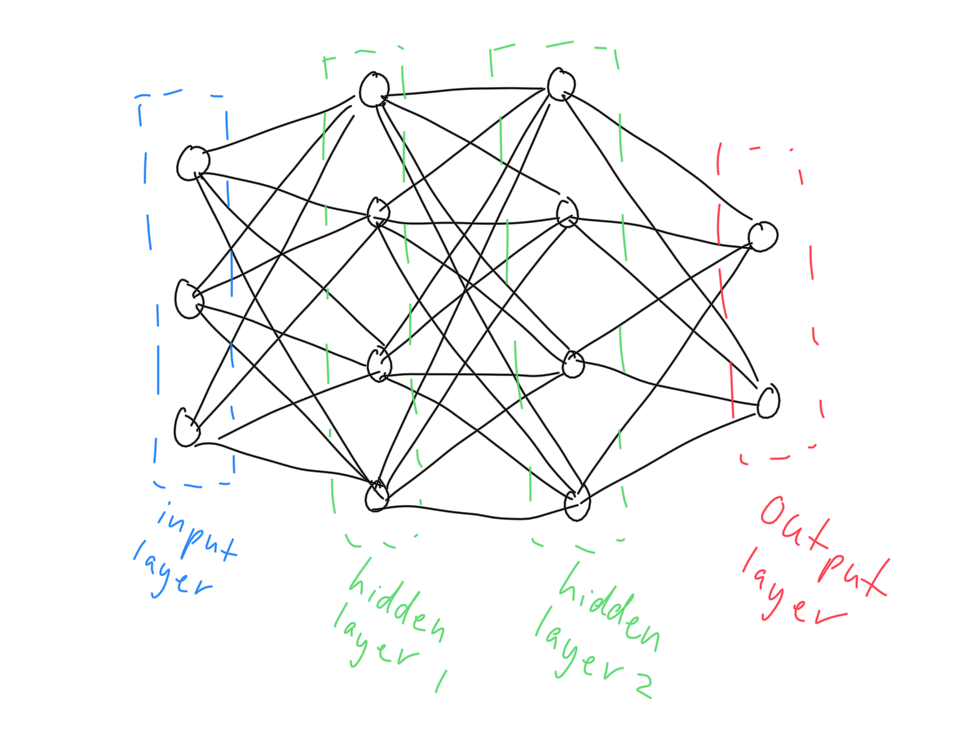
\includegraphics[width=0.5\paperwidth]{old/basic-nn.png}
    \caption{Simple Neural Network.}
    \label{fig:basic-nn}
\end{figure}

Looking at Figure \ref{fig:basic-nn}, we see that a feed-forward neural network is a series of connected \textbf{layers} that transform an input data point $\textbf{x}$ into an output data point $\textbf{y}$. Each layer is composed of \textbf{nodes}, the small black circles. Each node in the input layer corresponds to one dimension of a single data point $\textbf{x}$ (meaning the first node is $x_1$, the second node $x_2$, etc.). The same is true of the nodes in the output layer, which represent each dimension of $\textbf{y}$.  For a binary classification problem there is a single output node, representing the predicted probability of the positive class (with $K$ outputs for multi-classification). For a regression problem there may one or more nodes, depending on the dimensions of the output.  The nodes in the  \textbf{hidden} layers correspond to  \textbf{activation functions}.

\begin{figure}
    \centering
    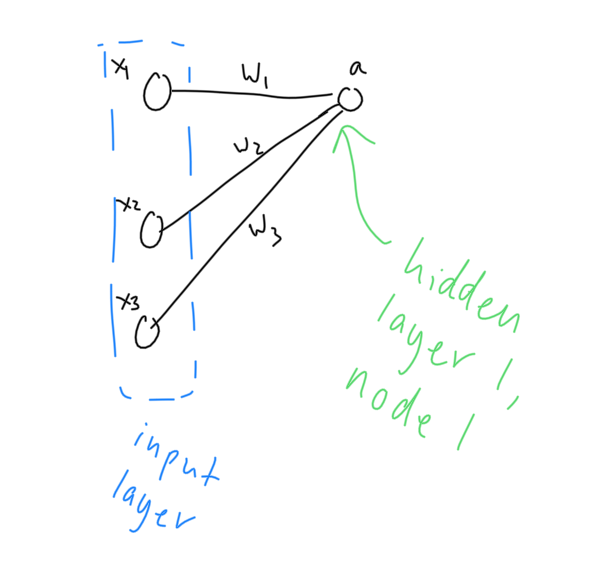
\includegraphics[width=0.5\paperwidth]{old/layer-one-node-one.png}
    \caption{Zooming in on the inputs and the first node of the first layer.}
    \label{fig:layer-one-node-one}
\end{figure}

 Let's zoom in on the first node in hidden layer 1, shown in Figure \ref{fig:layer-one-node-one}, to describe what happens at each node as we transform an input. For now we adopt simple notation and don't worry about indexing by later.
Looking at Figure \ref{fig:layer-one-node-one}, notice that every node in the input layer is connected to this first node in hidden layer 1. Each of the lines is a \textbf{connection}, that has a weight $w_{d}$ associated with it. We multiply all the nodes in the input layer by their corresponding weight, and then add them all together to produce the {\em activation} $a$, i..e,  the input at this first node (we've included the bias term in the input vector):
\begin{equation}
	a = x_{1} w_{1} + x_{2} w_{2} + x_{3} w_{3}
\end{equation}
\begin{warning}
    Every node in every layer has distinct weights associated with it.
\end{warning}

This gives us the activation for the first node in the first hidden layer. Once we've done this for every node in the first hidden layer, we make a non-linear transform of these activations, and then move on to computing the activations for the second hidden layer (which require the outputs from the first hidden layer, as indicated by the network of connections). We keep pushing values through the network in this manner until we have our complete output layer, at which point we are finished.

We've skipped over some important details in this high-level overview, but with this general information about what a neural network looks like and the terminology associated with it, we can now dig into the details a little deeper.

\subsection{Adaptive Basis Functions}
As we mentioned in the introduction, the strength of neural networks is that we can learn an effective basis for our problem domain at the same time as we train the parameters of our model. In fact, learning this basis becomes just another part of our parameter training. Let's make this notion of learning a basis more concrete.

Thinking back to our chapter on linear regression, we were training a model that made predictions using a functional form that looked like:
\begin{align*}
	y(\textbf{x}, \textbf{w}) = \textbf{w} \boldsymbol{\phi}^{T} = \sum_{d=1}^{D} w_{d} \boldsymbol{\phi}_{d}
\end{align*}
where $\boldsymbol{\phi} = \phi(\textbf{x})$, $\phi$ is the basis transformation function, and $D$ is the dimensionality of the data point.

Typically with this linear regression setup, we are training our model to optimize the parameters $\textbf{w}$. With neural networks this is no different--- we still train to learn those parameters. However, the difference in the neural network setting is that the basis transformation function $\phi$ is no longer fixed. Instead, the transformations are incorporated into the model parameters, and thus learned at the same time.

This leads to a different functional form for neural networks. A neural network with $M$ nodes in its first hidden layer  performs $M$ linear combinations of an input data point $\textbf{x}$:
\begin{equation} \label{basic-nn-form}
	a^{(1)}_{j} = \sum_{d=1}^{D} w_{jd}^{(1)} x_{d} + w_{j0}^{(1)} \quad \forall j \in 1..M
      \end{equation}

      Here, we use $a^{(1)}$ to denote the activation of a unit in layer 1 and notation $w^{(1)}$  denotes the weights used to determine the activations in layer 1. We also make the bias explicit.
      We will still use the bias trick in general, but we've left it out here to
      explicitly illustrate the bias term
      $w_{j0}^{(1)}$.
      %
      Other than this,  equation \ref{basic-nn-form} describes what we've already seen in Figure \ref{fig:layer-one-node-one}. The only difference is that we index each node in the hidden layer (along with its weights) by $j$.
      %There are $M$ nodes in this first hidden layer, corresponding to the $M$ linear combinations of the input data point $\textbf{x}$.
      %The notation $w^{(1)}$ indicates that these weights are part of the first hidden layer of our network.

      %Notice also that we haven't applied the `bias trick' of appending a $1$ to our data point $\textbf{x}$.
      
      The $M$ different values $a^{(1)}_{j}$ are the  activations. We transform these activations with a non-linear activation function $h(\cdot)$ to give:
      %
\begin{equation} \label{basic-nn-z-outputs}
	z^{(1)}_{j} = h(a_{j})
      \end{equation}
      
\begin{warning}
    Note that we didn't mention activation functions in the previous section only for the sake of simplicity. These non-linearities are crucial to the performance of neural networks because they allow for modeling of outcomes that vary non-linearly with their input variables.
\end{warning}

These values $z^{(1)}_{j}$ correspond to the outputs of the hidden units, each of which is associated with an activation function. Superscript $^{(1)}$ indicates they are the outputs of units in layer 1.
A typical activation function is the  sigmoid function, but  other common choices are the {\em tanh function} and {\em  rectified linear unit (ReLU)}.

These output values $z^{(1)}_{j}$, for units $j\in \{1,\ldots,M\}$ in layer 1,
form the inputs to the next layer. The activation of unit $j'$ in layer 2 depends on the outputs from layer 1 and the weights $w^{(2)}_{j'0},w^{(2)}_{j'1},\ldots,w^{(2)}_{j'M}$ that define the linear sum at the input of unit $j'$:
%
\begin{equation} \label{basic-nn-form-next-layer}
	a^{(2)}_{j'} = \sum_{j=1}^{M} w_{j'm}^{(2)} z^{(1)}_{j} + w_{j'0}^{(2)}
      \end{equation}
      
      We can connect many layers together in this way. They need not all have the same number of nodes but we will adopt $M$ for the number of nodes in each layer for convenience of exposition. Eventually, we will reach the output layer, and each output is denoted $y_{k}$, for $k\in \{1,\dots,K\}$.
      %
      The final activation function may be the sigmoid function, softmax function, or  just linear (and thus no transform).
      
We can now examine a more complete diagram of a feed-forward neural network, shown in Figure \ref{fig:feed-foward-nn}. It may be helpful to reread the previous paragraphs and use the diagram to visualize how a neural network transforms its inputs. This is a single hidden layer, or two-layer, network. Here, we use $z$ to denote the output values of the units in the hidden layer.

\begin{figure}
    \centering
    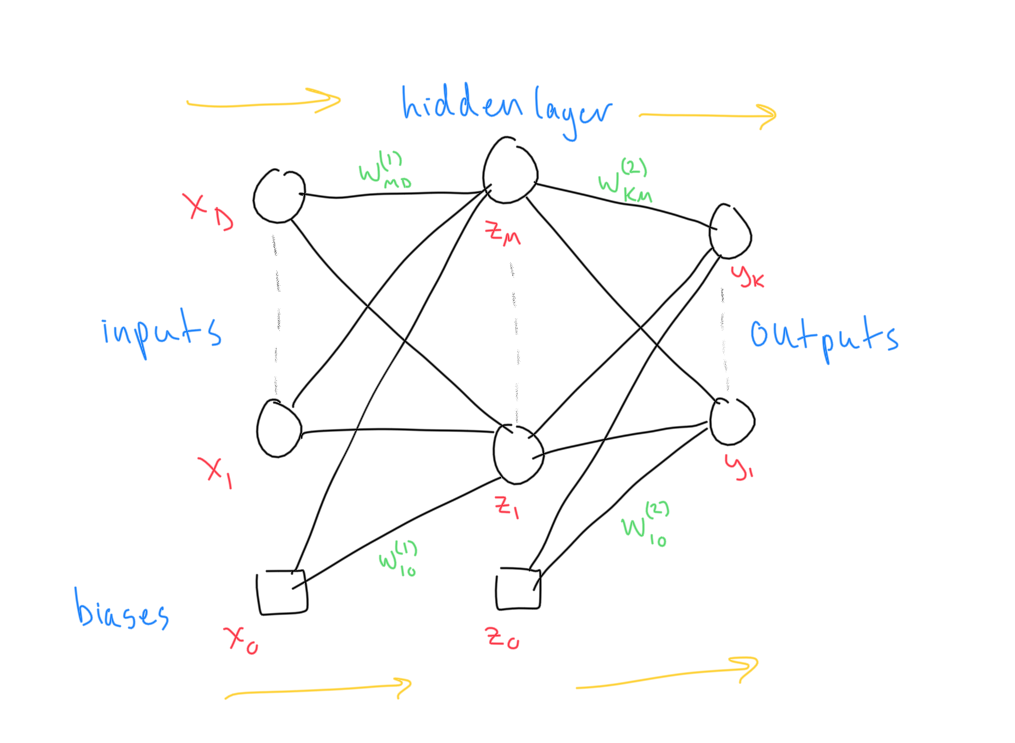
\includegraphics[width=0.5\paperwidth]{old/feed-forward-nn.png}
    \caption{Feed-Forward Neural Network.}
    \label{fig:feed-foward-nn}
\end{figure}

\begin{warning}
    Different resources choose to count the number of layers in a neural net in different ways. We've elected to count each layer of non-input nodes, thus the two-layer network in Figure \ref{fig:feed-foward-nn}. However, some resources will choose to count every layer of nodes (three in this case) and still others count only the number of hidden layers (making this a one layer network).
\end{warning}. 

Combining Figure \ref{fig:feed-foward-nn} and our preceeding functional description, we can describe the operation performed by a two-layer neural network using a single functional transformation (with $m$ to index a unit in the hidden layer):
%
\begin{equation} \label{full-nn-equation}
	y_{k}(\textbf{x}, \textbf{w}) = \sigma\bigg(\sum_{m=1}^{M}w_{km}^{(2)} h\bigg(\sum_{d=1}^{D}w_{md}^{(1)}x_{d} + w_{m0}^{(1)}\bigg) + w_{k0}^{(2)}\bigg)
\end{equation}
where we've elected to make the final activation function the sigmoid function $\sigma(\cdot)$, as is suitable for binary classification.  We use $h$ to denote the non-linear activation function for a hidden unit.
%
Written like this, a neural network is simply a non-linear function that transforms an input $\textbf{x}$ into an output $\textbf{y}$ that is controlled by our set of parameters $\textbf{w}$.

Furthermore, we see now why this  basic variety of neural networks is a \textit{feed-forward neural network}. We're  simply feeding our input \textbf{x} forward through the network from the first layer to the last layer. Assuming we have a fully trained network, we can make predictions on new input data points by propagating them through the network to generate output predictions (``the forward pass'').

We can also simplify this equation by utilizing the bias trick and appending an $x_{0}=1$ value to each of our data points such that:
\begin{equation*}
	y_{k}(\textbf{x}, \textbf{w}) = \sigma\bigg(\sum_{m=1}^{M}w_{km}^{(2)} h\bigg(\sum_{d=1}^{D}w_{md}^{(1)}x_{d}\bigg)\bigg)
\end{equation*}

Finally, it's worth considering that while a neural network is a series of linear combinations, it is special because of the differentiable non-linearities applied at each of the hidden layers. Without these non-linearities, the successive application of different network weights would be equivalent to a single large linear combination.

%Now that we understand the basic structure of a neural network, the important question of how to train our network remains. This is the topic we turn to next.

\section{Network Training}
Now that we understand the structure of a basic feed-forward neural network and how they can be used to make predictions, we turn our attention to the training process.

\subsection{Objective Function}

To train our network, it's first necessary to establish an objective function. Remember that neural networks can be used to solve both regression and classification problems, which means that our choice of objective will depend on the type of problem and the properties we desire.

For the case of {\em linear regression}, a common objective function is the {\em least squares loss}:
%
\begin{equation} \label{least-squares-loss-function}
	\mathcal{L}(\textbf{w}) = \frac{1}{2} \sum_{n=1}^{N} \bigg(y(\textbf{x}_{n}, \textbf{w}) - y_n\bigg)^{2},
      \end{equation}
      %
      where $y_n$ is the target value on example $n$. Sometimes we will have a regression problem with multiple outputs, in which case the loss would also take the sum over these different target values.
      
      For a {\em binary classification} problem, which we model through a single, sigmoid output activation unit,
     then  negated log-likelihood (or cross-entropy) is the typical  loss function:
      %
\begin{equation} \label{cross-entropy-loss-function}
	\mathcal{L}(\textbf{w}) = - \sum_{n=1}^{N} \bigg(y_{n}\ln{\hat{y}_{n}} + (1 - y_{n})(\ln{(1 - \hat{y}_{n})}\bigg)
      \end{equation}
      
      For a {\em multiclass classification problem}, produced by a softmax function in the output activation layer, we
      would use the negated log likelihood (cross entropy) loss:
\begin{equation} \label{multiclass-cross-entropy-loss-function}
	\mathcal{L}(\textbf{w}) = - \sum_{n=1}^{N} \sum_{k=1}^{K} y_{kn} \ln{\bigg(\frac{\text{exp}(a_{k}(\textbf{x}, \textbf{w}))}{\sum_{j=1}^{K}\text{exp}(a_{j}(\textbf{x}, \textbf{w}))}\bigg)}
\end{equation}

\begin{warning}
    Loss function and  objective function all refer to the same concept: the function we optimize to train our model.
\end{warning}

\subsection{Optimizing Parameters}

We want to find weight parameters \textbf{w} to minimize the objective function. The highly non-linear nature of neural networks means that this objective function will be non-convex with respect to our weight parameters. But still, we make use of stochastic gradient descent for optimization (refer to the previous chapter for a refresher).

In order to use gradient descent, we first need to figure out how to compute the gradient of our objective function with respect to our weights. That is the topic of the next section.

\subsection{Backpropagation}

Considering how our feed-forward neural network works, by propagating activations through our network to produce a final output, it's not immediately clear how we can compute gradients for the weights that lie in the middle of our networ. There is an elegant solution to this, which comes from ``sending errors backwards'' through our network, in a process known as \textit{backpropagation}.

\begin{definition}{Backpropagation}{backpropagation}
  
Backpropagation is the procedure by which we pass errors backwards through a feed-forward neural network in order to compute gradients for the weight parameters of the network.
\end{definition}

Backpropagation refers specifically to the portion of neural network training during which we compute the derivative of the objective function with respect to the weight parameters. This is done by propagating errors backwards through the network, hence the name.

\begin{warning}
    Note that we still need to update the value of the weight parameters after computing their derivatives. This is typically done using gradient descent or some variant of it.
\end{warning}

We now explore the details of backpropagation in greater depth.

\subsection{Computing Derivatives Using Backpropagation}

Recall that the activation $a_{j}^{(\ell)}$ for a  node $j$ in layer $\ell$ of a neural network can be described by the equation:
\begin{equation} \label{activations-reminder}
	a_{j}^{(\ell)} = \sum_{m=1}^{M} w^{(\ell)}_{jm} z^{(\ell-1)}_{m},
      \end{equation}
      % hull
where there are $M$ incoming nodes, each with corresponding output values $z^{(\ell-1)}_{1}, ..., z^{(\ell-1)}_{M}$, and with the weights in layer $\ell$ corresponding to node $j$ denoted by $w^{(\ell)}_{j1}, ..., w^{(\ell)}_{jM}$.
This activation is transformed by an activation function $h(\cdot)$  to give unit output $z^{(\ell)}_{j}$:
\begin{equation} \label{transformed-activations-reminder}
	z^{(\ell)}_{j} = h(a^{(\ell)}_{j}).
\end{equation}

Computing these values as we flow through the network constitutes the {\em forward pass } through our network.

We now wish to begin the process of computing derivatives of the objective function with respect to our weights. For the sake of simplicity, we'll assume that the current setting of our parameters $\textbf{w}$ generates a loss of $L$ for a single data point, as though we were performing stochastic gradient descent.

Let's consider how we could compute the derivative of $L$ with respect to an individual weight in our network, $w^{(\ell)}_{jm}$ (the $m$th weight for activation $j$ in layer $\ell$):
%
\begin{equation} \label{deriv-E-wrt-wjm}
	\frac{\partial L}{\partial w^{(\ell)}_{jm}}.
\end{equation}

We first need to figure out what the dependence of $L$ is on this weight. This weight contributes to the final result only via its contribution to the activation $a^{(\ell)}_{j}$. This allows us to use the chain rule to simplify Equation \ref{deriv-E-wrt-wjm} as:
%
\begin{equation} \label{chain-rule-deriv-E-wrt-wjm}
	\frac{\partial L}{\partial w^{(\ell)}_{jm}} = \frac{\partial L}{\partial a^{(\ell)}_{j}} \cdot \frac{\partial a^{(\ell)}_{j}}{\partial w^{(\ell)}_{jm}}.
      \end{equation}

      The first part of this is the, typically non-linear, dependence of loss on activation. The second part is the linear dependence of activation on weight.
      %
Using Equation \ref{activations-reminder}, we have that:
\begin{equation*}
	\frac{\partial a^{(\ell)}_{j}}{\partial w^{(\ell)}_{jm}} = z^{(\ell-1)}_{m},
\end{equation*}

and just the value of the input from the previous layer. We now introduce the following notation for the first term,
%
\begin{equation} \label{delta-expression}
	\delta^{(\ell)}_{j} = \frac{\partial L}{\partial a^{(\ell)}_{j}},
\end{equation}
where $\delta^{(\ell)}_{j}$ values are referred to as \textit{errors}. We rewrite Equation \ref{chain-rule-deriv-E-wrt-wjm} as:
%
\begin{equation} \label{simplified-chain-rule-deriv-E-wrt-wjm}
	\frac{\partial L}{\partial w^{(\ell)}_{jm}} = \delta^{(\ell)}_{j} z^{(\ell-1)}_{m}.
\end{equation}

The implications of Equation \ref{simplified-chain-rule-deriv-E-wrt-wjm} are significant for understanding backpropagation.  The derivative of the loss with respect to an arbitrary weight in the network
can be calculated as the product of the error $\delta^{(\ell)}_j$ at the ``output end of that weight'' and the value $z^{(\ell-1)}_m$ at the ``input end of the weight.''  We visualize this property in Figure \ref{fig:backprop-gradient} (dropping the layer subscripting).
%
\begin{figure}
    \centering
    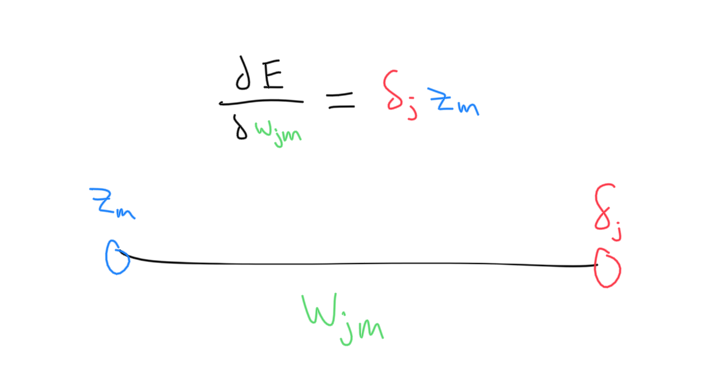
\includegraphics[width=0.5\paperwidth]{old/backprop-gradient.png}
    \caption{Gradient of the loss function in a neural network with respect to a weight. It depends on the input value $z_m$ and the ``error'' corresponding to the activation value at the output end of the weight.}
    \label{fig:backprop-gradient}
\end{figure}

To compute the derivatives, it suffices to compute the values of $\delta_{j}$ for each node, also saving the output values  $z_{m}$ during the forward pass through the network (to be multiplied by the values of $\delta_{j}$ to get partials).

\begin{warning}
    We will only have ``errors values'' $\delta_{j}$ for the hidden and output units of our network. This is logical because there is no notion of applying an error to our input data, which we have no control over.
\end{warning}

We now consider how to compute these error values.  For a unit in the output layer, indexing it here by $k$,  and assuming the output activation function is linear and adopting least squares loss (i.e., regression), we have  for the dependence of loss on the activation of this unit,
%
\begin{equation*}
  \delta^{(\ell)}_{k} = \frac{\partial L}{\partial a^{(\ell)}_k} =
 \frac{\partial L}{\partial \hat{y}_k} =
  \frac{\mathrm{d} \big( \frac{1}{2}(\hat{y}_k- y_k)^2 \big)}{\mathrm{d} \hat{y}_{k}} = \hat{y}_{k} - y_{k}.
\end{equation*}

Here, we use shorthand $a^{(\ell)}_k=\hat{y}_k$, providing the $k$th dimension of the  prediction  of the  model. Although a regression problem, we're imagining here that there are multiple regression targets (say, the height, weight and blood pressure of an individual). Here, $y_k$ is the true target value for this data point. Note that this is for OLS. The expression would be different for a classification problem and negated log likelihood as the loss.

\if 0
The error $\delta_k^{(\ell)}$ on a unit in the output layer, for this case of OLS, is the difference between the output of the network and the target value. We've seen this term, the difference between the expected and actual results, arise in the gradient of our error expressions for both linear regression and classification.
\fi

To compute the error $\delta^{(\ell)}_{j}$ for a hidden unit $j$ in a layer $\ell$, we again make use of the chain rule, and write:
%
\begin{equation} \label{backprop-for-deltas}
	\delta^{(\ell)}_{j} = \frac{\partial L}{\partial a^{(\ell)}_{j}} = \sum_{m=1}^{M} \frac{\partial L}{\partial a^{(\ell+1)}_{m}} \frac{\partial a^{(\ell+1)}_{m}}{\partial a_{j}^{(\ell)}}, 
\end{equation}
where the summation runs over all of the $M$ nodes to which the node $j$ in layer $\ell$ sends connections, as seen in Figure \ref{fig:sum-over-nodes}. This expression recognizes that the activation value of this unit contributes only via its contribution to the activation value of each unit to which it is connected in the next layer. The first term in
one of the  products in the summation is the, typically non-linear, dependence between loss and activation value of a unit in the next layer. The second term in one of the products captures the relationship between this activation and the subsequent activation.
%
%
\begin{figure}
    \centering
    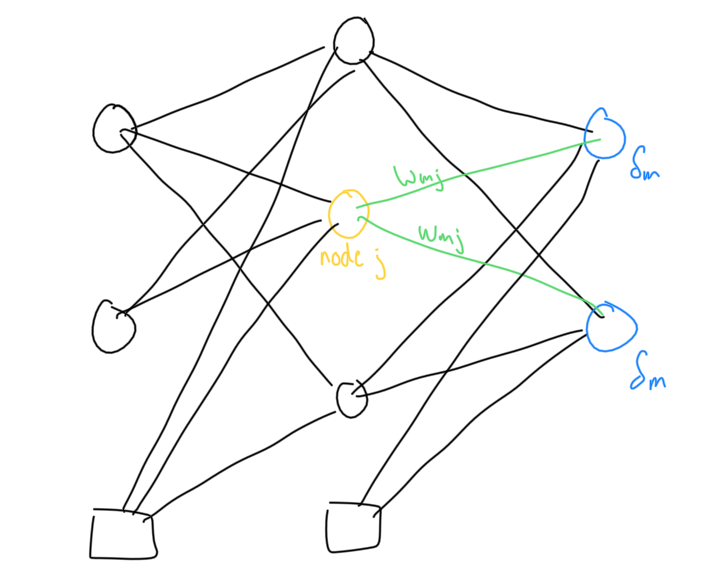
\includegraphics[width=0.5\paperwidth]{old/sum-over-nodes.png}
    \caption{Summation over the nodes (blue) in layer $\ell+1$ to which node $j$ in layer $\ell$ (gold) sends connections (green). Note: read this as $m$ and $m'$.}
    \label{fig:sum-over-nodes}
\end{figure}

Now, we can simplify by noticing that:
%
\begin{align}
  \frac{\partial L}{\partial a_m^{(\ell+1)}}&=\delta^{(\ell+1)}_m \quad\quad\mbox{\{by definition\}}\\
  \frac{\partial a_m^{(\ell+1)}}{\partial a_j^{(\ell)}}&=\frac{\mathrm{d}h(a_j^{(\ell)})}{\mathrm{d}a_j^{(\ell)}}\cdot w^{(\ell+1)}_{mj}=h'(a_j^{(\ell)})\cdot w_{mj}^{(\ell+1)}. \quad\quad\mbox{\{chain rule\}}
\end{align}

Substituting, and pulling forward the derivative of the activation function, we can rewrite the expression for the error on a hidden unit $j$ in layer $\ell$ as:
%
\begin{equation} \label{backprop-formula}
	\delta^{(\ell)}_{j} = h'(a^{(\ell)}_{j}) \sum_{m=1}^{M} w^{(\ell+1)}_{mj} \delta^{(\ell+1)}_{m}.
      \end{equation}

      This is very useful, and is the key insight in backpropagation.  It means that the value of the errors  can be computed by ``passing back'' (backpropagating) the errors for  nodes farther up in the network!
%
Since we know the values of $\delta$ for the final layer of output node, we can recursively apply Equation \ref{backprop-formula} to compute the values of $\delta$ for all the nodes in the network.

Remember that all of these calculations were done for a single input data point that generated the loss $L$. If we were using SGD with  mini-batches, then we would perform  same calculation for each data point in mini-batch $B$, and average the gradients as follows:
%
\begin{equation} \label{batch-errors-backprop}
	\frac{\partial L}{\partial w^{(\ell)}_{jm}} = \frac{1}{|B|}\sum_{n\in B} \frac{\partial L_{n}}{\partial w^{(\ell)}_{jm}},
      \end{equation}
      %
      where $L_n$ is the loss on example $n$.
     
To solidify our understanding of the backpropagation algorithm, it can be useful to try a concrete example.
%
\begin{example}{Backpropagation Example}{backprop-example}
  Imagine the case of a simple two layer neural network as in Figure \ref{fig:feed-foward-nn}, with $K$ outputs (we denote them $\hat{y}_1$ through $\hat{y}_K$ for a given data point). We imagine this is a regression problem, but one
  with multiple dimensions to the output, and assume OLS. For a given data point, the loss is computed as:
   %
	\begin{align*}
		L = \sum_{k=1}^{K} \frac{1}{2}(\hat{y}_{k} - y_{k})^{2},
	\end{align*}
        %
        where we write $y_k$ for the $k$th dimension of the target value.
%
        For a unit in the hidden layer, with activation value $a$, we make use of the sigmoid activation, with 
        %
	\begin{align*}
z=		\sigma(a) = \frac{1}{1 + \exp{(-a)}},
	\end{align*}
	whose derivative is given by:
	\begin{align*}
		\frac{\partial \sigma(a)}{\partial a} = \sigma(a)(1 - \sigma(a)).
	\end{align*}
        
	For an input data point $\textbf{x}$, we forward propagate through the network to get the activations of the hidden layer, and for each $m$ in this layer we have:
	\begin{align*}
		a_{m}^{(1)} = \sum_{d=0}^{D} w^{(1)}_{md} x_{d},
	\end{align*}
    given weights $w^{(1)}_{m0},\ldots, w^{(1)}_{mD}$,   and  with output value from unit $m$ as, 
%
	\begin{align*}
		z^{(1)}_{m} = \sigma{(a^{(1)}_{m})}.
	\end{align*}
        
	We propagate these output values  forward to get the outputs, and for each output unit $k$, we have:
	\begin{align*}
		\hat{y}_{k} = \sum_{m=0}^{M} w_{km}^{(2)} z^{(1)}_{m},
	\end{align*}
        %
where $w^{(2)}_{k0},\ldots,w^{(2)}_{kM}$ are the weights for unit $k$.
        
	Now that we've propagated forward, we propagate our errors backwards! We start by computing the errors for the output layer as follows:
	\begin{align*}
		\delta^{(2)}_{k} =  \frac{\partial L}{\partial \hat{y}_k}=\hat{y}_{k} - y_{k}.
	\end{align*}

	We then backpropagate these errors back to each hidden unit $m$ in layer 1 as follows:
	\begin{align*}
          \delta^{(1)}_{m} = \frac{\partial L}{\partial a_m^{(1)}} & =
                                                                     h'(a_m^{(1)})\sum_{k=1}^Kw^{(2)}_{km}\delta^{(2)}_k\\
                                                                   &=\sigma(a^{(1)}_m)(1-\sigma(a^{(1)}_m))\sum_{k=1}^Kw^{(2)}_{km}(\hat{y}_k-y_k)\\
                                                                   &=z_m^{(1)}(1-z_m^{(1)}) \sum_{k=1}^Kw^{(2)}_{km}(\hat{y}_k-y_k).
                                                                     \end{align*}

	And now that we have our errors for the hidden and output layers, we can compute the derivative of the loss with respect to our weights as follows, for the $d$th weight on the $m$th unit in layer 1, and the $m$th weight on the $k$th unit in layer 2: 
	\begin{align*}
		\frac{\partial L}{\partial w_{md}^{(1)}} = \delta^{(1)}_{m} x_{d}, \quad \frac{\partial L}{\partial w^{(2)}_{km}} = \delta^{(2)}_{k} z^{(1)}_{m}.
	\end{align*}
        
	We then use these derivatives along with an optimization technique such as stochastic gradient descent to improve the model weights.
\end{example}

\section{Choosing a Network Structure}
Now that we know the general form of a neural network and how the training process works, we must step back and consider the question of how we actually arrive at an optimal network structure. We'll begin with an idea we've already seen before: cross validation.

\subsection{Cross Validation for Neural Networks}
We've previously discussed cross validation in the chapter on linear regression. We used it then to compare the performance of different models, attempting to identify the best model while also avoiding overfitting. We can use a similar process to identify a reasonable network structure.

First of all, the input and output parameters of a neural network are generally decided for us: the dimensionality of our input data dictates the number of input units and the dimensionality of the required output dictates the number of output units. For example, if we have an 8-by-8 pixel image and need to predict whether it is a `0' or a `1', our input dimensions are fixed at 64 and our output dimensions are fixed at 2. Depending on whether you wish to perform some sort of pre or post-processing on the inputs/outputs of your network, this might not actually be the case, but in general when choosing a network structure we don't consider the first or last layer of nodes as being a relevant knob that we can tune.

That leaves us to choose the structure of the hidden layers in our network. Unsurprisingly, the more hidden layers we have and the more nodes we have in each of those layers, the more variation we will produce in our results and the closer we will come to overfitting.

Thus, we can use cross validation in the same way we've done before: train our model with differing numbers of internal units and structures (as in Figure \ref{fig:internal-node-differences}) and then select the model that performs best on the validation set.

\begin{figure}
    \centering
    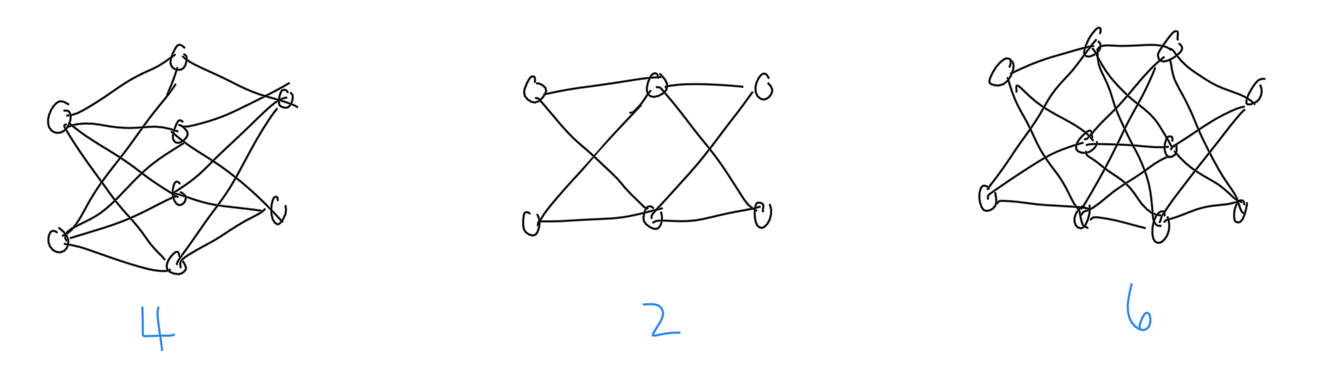
\includegraphics[width=0.5\paperwidth]{old/internal-node-differences.png}
    \caption{Networks with different structures and numbers of internal nodes.}
    \label{fig:internal-node-differences}
\end{figure}

\begin{warning}
    There are other considerations at play beyond performance when choosing a network structure. For example, the more internal units you have in your network, the more storage and compute time you will need to train them. If either training time or response time after training a model is critical, you may need to consider consolidating your network at the expense of some performace.
\end{warning}

\subsection{Preventing Overfitting}
Besides keeping your neural network small, there are other means of preventing it from overfitting.

\subsubsection{Regularization}
You can also apply regularization to the weights in your network to help prevent overfitting. For example, we could introduce a simple quadratic regularizer of the form $\frac{\lambda}{2} \textbf{w}^{T}\textbf{w}$ to our objective function. There are other considerations to be made here, for example we would like our regularizer to be invariant to scaling, meaning that multiplying our input data by a constant would produce a proportionally equivalent network after training. The quadratic regularizer is not invariant to scaling, but the basic concept of avoiding extreme weights is the same nonetheless.

\subsubsection{Data Augmentation}
We can use transformations to augment our data sets, which helps prevent overfitting. This technique is not specific to neural networks, but often the types of unstructured data for which we use neural networks can benefit greatly from it.
\begin{definition}{Data Augmentation}{data-augmentation}
Data augmentation refers to the practice of increasing the size and diversity of your training data by applying transformations to the initial data set.
\end{definition}
For example, if we are working with image data, we might choose to rotate or reflect the image, depending on the type of network we are trying to build and whether or not this would preserve the integrity of the image. We might also change something like the brightness or density of the image data. In this way, we can produce more and more varied training points, thus reducing the likelihood of overfitting.

\section{Specialized Forms of Neural Networks}
Simple neural networks are useful for a general set of tasks, and as universal function approximators, they \textit{could} be useful for any task. However, there are certain data types and use cases for which we've developed more specialized forms of neural networks that perform even better in their respective domains. We will take a high level view of these different flavors of neural networks.

\subsection{Convolutional Neural Networks (CNNs)}
Convolutional neural networks (abbreviated CNNs) are most often used for image data, but their underlying principles apply in other domains as well.

To understand why a CNN is useful, consider this specific problem: you are trying to determine whether or not there is a dog in an image. There are two general difficulties we have to deal with in solving this problem. First, while dogs have a lot of similar features (ears, tails, paws, etc.), we need some means of breaking an image down into smaller pieces that we can identify as being ears or tails or paws. Second, what happens if we train on images of dogs that are all in the center of the photo, and then we try to test our network on an image where the dog is in the upper left hand corner? It's going to fail miserably.

CNNs overcome these problems by extracting smaller local features from images via what's known as a \textit{sliding window}. You can imagine this sliding window as a matrix kernel that moves over every subsection of an image, producing a summary of those subsections that feed into the next layer in our network. We do this over the entire image, and with several different sliding windows. Without going into too many details, this solves the two general problems we had above: our small sliding window can summarize a feature of interest (such as a dog ear) and it is also location invariant, meaning that we can identify that dog ear anywhere in an image.

\begin{figure}
    \centering
    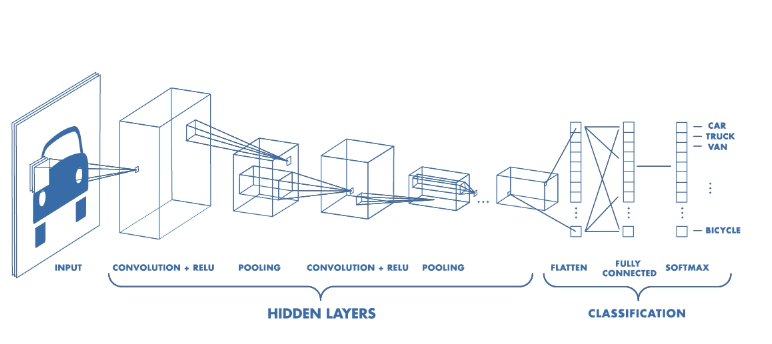
\includegraphics[width=0.5\paperwidth]{old/CNN-structure.png}
    \caption{Excellent diagram of the structure of a CNN. source: https://www.mathworks.com/videos/introduction-to-deep-learning-what-are-convolutional-neural-networks--1489512765771.html}
    \label{fig:CNN-structre}
\end{figure}

\subsection{Recurrent Neural Networks (RNNs)}
As with CNNs, recurrent neural networks (abbreviated RNNs) are used to more efficiently solve a specific problem type. To motivate the structure of an RNN, we will turn again to a specific example.

Imagine we were building a tool with the goal of predicting what word comes next in a newspaper article. Obviously, the words that came before the word that we are currently trying to predict are crucial to predicting the next word. Imagine we propagate the preceding ten words through our network to predict which word we think will come next. It would also be useful if we could send some of the information at each layer backwards through the network to help with the next prediction - since we know the sequence of words matters. In this sense, our network is `stateful' because it's remembering what came before. We don't have this ability with a feed-forward network, which by design only propagates information forward through the network. RNNs add backward passing of activations into their network structure to improve predictions on data where there is some temporal dependence on what came previously.

\begin{figure}
    \centering
    
\includegraphics[width=0.5\paperwidth]{old/RNN-structure.png}
    \caption{Simple example of an RNN.}
    \label{fig:RNN-structre}
\end{figure}


\subsection{Bayesian Neural Networks (BNNs)}
Up until now, our training process has been one of maximum likelihood estimation, or a maximum posterior approach if we utilize a regularizer that can be interpreted as introducing a prior.

A Bayesian neural network, or BNN, does exactly what you might imagine: it introduces a distribution over the parameters of our model, which then requires marginalizing over those distributions in order to make a prediction. The specifics of how exactly a BNN is constructed are beyond the scope of this textbook, but the idea behind why we would utilize a BNN is the same as the reason we utilize Bayesian techniques in other domains, particularly the use of prior information to aid model performance.

  % \chapter{Support Vector Machines}
In this chapter, we will explore what are known as a support vector machines, or SVMs for short. SVMs are broadly useful for problems in classification and regression, and they are part of a family of techniques known as \textit{margin methods}. The defining goal of margin methods, and SVMs specifically, is to put as much distance as possible between data points and decision boundaries. We will dig deeper into what exactly this means over the course of the chapter. One of the most appealing aspects of SVMs is that they can be solved as convex optimization problems, for which we can find a global optimum with relative ease. We will explore the mathematical underpinnings of SVMs, which can be slightly more challenging than our previous topics, as well as their typical use cases.

\section{Motivation}
While SVMs can be used for classification or regression, we will reason about them in the classification case as it is more straightforward. 

The grand idea behind SVMs is that we should construct a linear hyperplane in our feature space that maximally separates our classes, which means that the different classes should be as far from that hyperplane as possible. The distance of our data from the hyperplane is known as \textit{margin}.

\begin{definition}[margin]
  Margin is the distance of the nearest data point from the separating hyperplane of an SVM model, as seen in Figure \ref{fig:2d-hyperplane}. Larger margins often lead to more generalizable models.
\end{definition}

A larger margin tends to mean that our model will generalize better, since it provides more wiggle room to correctly classify unseen data (think about new data being a perturbation on current data).

\begin{figure}
    \centering
    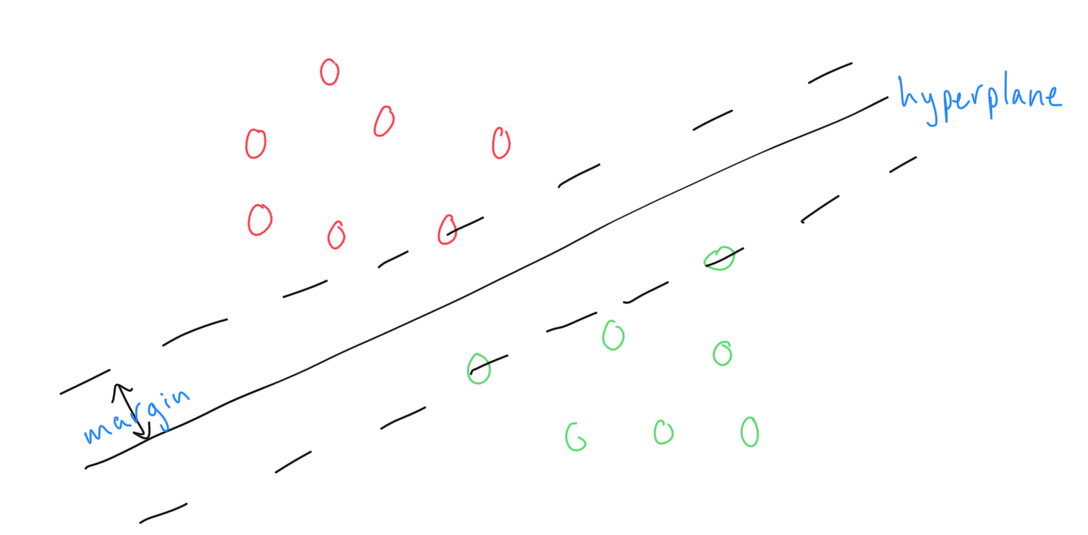
\includegraphics[width=0.5\paperwidth]{old/2d-hyperplane.png}
    \caption{Hyperplane with margin between different classes.}
    \label{fig:2d-hyperplane}
\end{figure}

This idea of the margin of a separator is quite intuitive. If you were presented with Figure \ref{fig:2d-hyperplane} and were asked to separate the two classes, you would likely draw the line that keeps data points as far from it as possible. SVMs and other margin-based methods will attempt to algorithmically recreate this intuition.

\subsection{Max Margin Methods}
SVMs are a specific instance of a broader class of model known as \textit{max margin methods}. Their name describes them well: they deal with creating a maximum margin between training data and decision boundary, with the idea that this leads to model generalizability. 

Other max margin methods are outside the scope of this textbook. These alternative methods may differ from SVMs in a non-trivial way. For example, SVMs do not produce probabilities  on different classes, but rather decision rules for handling new data points. If you needed probabilities, there are other max margin methods that can be used for the task.
%
\begin{mlcube}[support vector machines]{Discrete}{Supervised}{No}
SVMs are typically used in settings with discrete outputs. We need labeled training data to identify the relevant hyperplane in an SVM model. Finally, SVMs operate in a non-probabilistic setting.
\end{mlcube}

\subsection{Applications}
The theory behind SVMs has been around for quite some time (since 1963), and prior to the rise of neural networks and other more computationally intensive techniques, SVMs were used extensively for image recognition, object categorization, and other typical machine learning tasks.

SVMs are still widely used in practice, for example for  classification problems known as anomaly detection.
%
\begin{warning}
    The purpose of anomaly detection is to identify unusual data points. For example, if we are manufacturing shoes, we may wish to inspect and flag any shoe that seems atypical with respect to the rest of the shoes we produce.
\end{warning}

Anomaly detection can be as simple as a binary classification problem where the data set is comprised of anomalous and non-anomalous data points. As we will see, an SVM can be constructed from this data set to identify future anomalous points very efficiently. SVMs extend beautifully to settings where we want to use basis functions, and thus non-linear interactions on features. For this reason, they continue to be competitive in many real-world situations where these kinds of interactions are important to work with.

\section{Hard Margin Classifier for Linearly Separable Data}

We will learn the theory behind SVMs by starting with a simple two-class classification problem, as we've seen several times in previous chapters. We will constrain the problem even further by assuming, at least to get started, that the two classes are linearly separable, which is the basis of the \textit{hard margin} formulation for SVMs.

\begin{warning}
    The expression `hard margin' simply means that we don't allow any data to be classified incorrectly. If it's not possible to find a hyperplane that perfectly separates the data based on class, then the hard margin classifier will return no solution.
\end{warning}

\subsection{Why the Hard Margin}
The hard margin constraint, which assumes that our data is linearly separable, is not actually a requirement for constructing an SVM, but it simplifies the problem initially and makes our derivations significantly easier. After we've established the hard margin formulation, we will extend the technique to work in situations where our data is not linearly separable.

\subsection{Deriving our Optimization Problem}
Recall that our goal is to define a hyperplane that separates our data points and maintains the maximum possible distance between the hyperplane and nearest data points on either side of it.
There are  $N$ examples  $\textbf{x}_{1}, ..., \textbf{x}_{N}$ and there is a bias term $w_{0}$.
Each example has a label $y_{1}, ..., y_{N}$ which is either $1$ or $-1$. 
To uncover this hyperplane, we start with a simple linear model for a two-class classification problem:
\begin{equation} \label{classification-fn}
h(\textbf{x}) = \textbf{w}^\top \textbf{x} + w_{0}.
\end{equation}

This is the {\em discriminant function} and we classify a new example to class $1$ or $-1$ according to the sign produced by our trained model $h(\textbf{x})$. Later, we will also make this more general by using a basis function, 
$\phi(\mathbf{x})$ to transform to a higher dimensional feature space.

By specifying our model this way, we have implicity defined a hyperplane separating our two classes given by:
\begin{equation} \label{implicit-hyperplane}
	\textbf{w}^\top \textbf{x} + w_{0} = 0
\end{equation}
Furthermore, we have that $\textbf{w}$ is orthogonal to the hyperplane, which we demonstrate now:

\begin{derivation}[hyperplane orthogonal to $\textbf{w}$]
	Imagine two data points $\mathbf{x}_{1}$ and $\mathbf{x}_{2}$ on the hyperplane defined by $\textbf{w}^\top \textbf{x} + w_{0} = 0$. When we project their difference onto our model $\textbf{w}$, we find:
	\begin{equation} \label{hyperplane-eqn}
		\textbf{w}^\top(\textbf{x}_{1} - \textbf{x}_{2}) = \textbf{w}^\top\textbf{x}_{1} - \textbf{w}^\top\textbf{x}_{2} = -w_{0} - (-w_{0}) = 0
	\end{equation}
	which means that $\textbf{w}$ is orthogonal to our hyperplane. We can visualize this in Figure \ref{fig:orthogonal-w}.
\end{derivation}

\begin{figure}
    \centering
    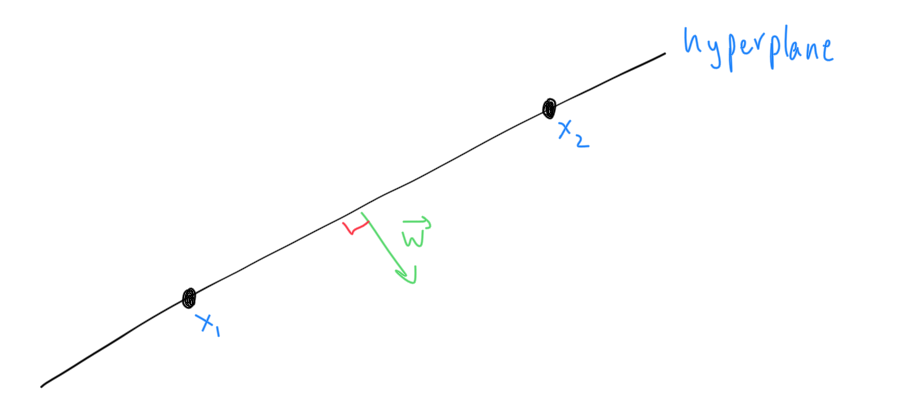
\includegraphics[width=0.5\paperwidth]{old/orthogonal-w.png}
    \caption{Our weight vector \textbf{w} is orthogonal to the separating hyperplane.}
    \label{fig:orthogonal-w}
\end{figure}

Remember that we're trying to maximize the margin between our training data and the hyperplane. The fact that $\textbf{w}$ is orthogonal to our hyperplane will help with this.

To determine the distance between a data point $\textbf{x}$ and the hyperplane, which we denote $d$, we need the distance in the direction of $\textbf{w}$ between the point and the hyperplane. We denote $\textbf{x}_{p}$ to be the projection of $\textbf{x}$ onto the hyperplane, which allows us to decompose $\textbf{x}$ as the following:
\begin{equation} \label{decompose-x}
	\textbf{x} = \textbf{x}_{p} + d \frac{\textbf{w}}{|| \textbf{w} ||_2}
\end{equation}
which is the sum of the portion of the projection of $\textbf{x}$ onto the hyperplane and the portion of $\textbf{x}$ that is parallel to $\textbf{w}$ (and orthogonal to the hyperplane). From here we can solve for $d$:
%
\begin{derivation}[Distance from Hyperplane Derivation]
	We start by left multiplying Equation \ref{decompose-x} with $\textbf{w}^\top$,
	\begin{align*}
		\textbf{w}^\top\textbf{x} = \textbf{w}^\top\textbf{x}_{p} + d \frac{\textbf{w}^\top\textbf{w}}{||\textbf{w}||_2}.
	\end{align*}
	Simplifying (note that $\textbf{w}^\top\textbf{x}_{p} = -w_{0}$ from Equation \ref{hyperplane-eqn}):
	\begin{align*}
		\textbf{w}^\top\textbf{x} =  - w_{0} + d ||\textbf{w}||_2
	\end{align*}
	Rearranging:
	\begin{align*}
		d = \frac{\textbf{w}^\top\textbf{x} + w_{0}}{||\textbf{w}||_2}.
	\end{align*}
\end{derivation}

For each data point $\textbf{x}$, we now have the signed distance of that data point from the hyperplane.

For an example that is classified correctly, this signed distance $d$ will be positive for class $y_n = 1$, and negative for class $y_n = -1$.  Given this, we can make the distance unsigned (and always   positive) for a correctly classified data point by multiplying by $y_n$. Then, the {\em margin for an correctly classified data point $(\textbf{x}_{n},y_n)$} is given by:
\begin{equation} \label{individual-margin}
	\frac{y_{n}(\textbf{w}^\top\textbf{x}_{n} + w_{0})}{||\textbf{w}||_2}.
      \end{equation}
      
      The margin for an entire data set is given by the margin to the closest point in the data set,  and
      %
\begin{equation} \label{total-margin}
	\min_{n} \frac{y_{n}(\textbf{w}^\top\textbf{x}_{n} + w_{0})}{||\textbf{w}||_2}.
\end{equation}

Then, it is our goal to maximize this margin with respect to our model parameters $\textbf{w}$ and $w_{0}$. This is given by:
\begin{equation} \label{total-maximized-margin}
  \underset{\textbf{w}, w_{0}}{\max}  \ \ \frac{1}{||\textbf{w}||_2} \left[\min_{n} y_{n}(\textbf{w}^\top\textbf{x}_{n} + w_{0}) \right]
\end{equation}

Here, we pull the $1/||\mathbf{w}||_2$ term forward. Note carefully that $w_0$ does not play a role in the denominator $||\mathbf{w}||_2$.

This is a hard problem to optimize, but we can make it more tractable by recognizing some important features of Equation \ref{total-maximized-margin}. First, rescaling $\textbf{w} \rightarrow \alpha \textbf{w}$ and $w_{0} \rightarrow \alpha w_{0}$, for any $\alpha >0$, has no impact on the margin for any correctly classified data point $\textbf{x}_{n}$. This is because the effect of $\alpha$ cancels out in the numerator and denominator of Equation~\ref{individual-margin}.

We can use this rescaling liberty to enforce
%
\begin{equation} \label{new-margin-constraint}
  y_{n}(\textbf{w}^\top\textbf{x}_{n} + w_{0}) \geq 1,  \quad \quad \mbox{for all $n$}.
\end{equation}

This does not change the optimal margin because we can always scale up both $\mathbf{w}$ and $w_0$ by $\alpha>0$ to achieve
$ y_{n}(\textbf{w}^\top\textbf{x}_{n} + w_{0}) \geq 1$, and without affecting the margin. Moreover, since the problem is to maximize $1/||\mathbf{w}||_2$, an optimal solution will want $||\mathbf{w}||_2$ to be as small as possible, and thus at
least one of these constraints~\eqref{new-margin-constraint} will be binding and equal to one  in an optimal solution. 

Thus our optimization problem now looks like:
\begin{equation} \label{simplified-maximized-margin-optimization}
	\underset{\textbf{w}, w_{0}}{\max} \ \ \frac{1}{||\textbf{w}||_2} \quad \text{s.t.} \quad y_{n}(\textbf{w}^\top\textbf{x}_{n} + w_{0}) \geq 1, \quad \mbox{for all $n$}.
      \end{equation}

      Here, we recognized that $\min_{n} y_{n}(\textbf{w}^\top\textbf{x}_{n} + w_{0})=1$ in an optimal solution with these new constraints,
      and adopted this in the objective.  This simplifies considerably, removing the ``min $_n$'' part of the objective.
      
Notice that maximizing $\frac{1}{||\textbf{w}||_2}$ is equivalent to minimizing $||\textbf{w}||_2^{2}$. We will also add a constant term $\frac{1}{2}$ for convenience, leaving the {\bf hard-margin formulation of the training problem}:
%
\begin{equation} \label{final-simplified-maximized-margin-optimization}
	\underset{\textbf{w}, w_{0}}{\min}\ \  \frac{1}{2} ||\textbf{w}||_2^{2} \quad \text{s.t.} \quad y_{n}(\textbf{w}^\top\textbf{x}_{n} + w_{0}) \geq 1, \quad \mbox{for all $n$}.
\end{equation}

Note that Equation \ref{final-simplified-maximized-margin-optimization} is now a quadratic programming problem, which means we wish to optimize a quadratic function subject to a set of linear constraints on our parameters. Arriving at this form was the motivation for the preceding mathematic manipulations. We will discuss shortly how we actually optimize this function.

\subsection{What is a Support Vector}

Up until now, we have discussed Support Vector Machines without identifying what a support vector is. We now have enough information from the previous section to define them. Later, when we work with a dual formulation, we will see the precise role that they play.

Say that an
example is on the {\em margin boundary}
if $y_{n}(\textbf{w}^\top\textbf{x}_{n} + w_{0}) =1$. These are the points that are closest to the hyperplane and have margin $1/||{\mathbf w}||_2$.
%
\begin{definition}[support vector]
  A support vector in a  hard-margin SVM  formulation  must be a data point that is on
  the margin boundary of the optimal solution, with $y_{n}(\textbf{w}^\top\textbf{x}_{n} + w_{0}) =1$ and margin $1/||{\mathbf w}||_2$.
\end{definition}

In the hard margin case we have constrained the closest data points to
have discriminant value $\textbf{w}^\top\textbf{x}_{n} + w_{0} = 1$ ($-1$ for a negative example).
Figure \ref{fig:hard-margin-svm} shows a hard margin SVM solution with an illustration of
corresponding support vectors.

\begin{warning}
  After we have optimized an SVM in the hard margin case, we must have at least two support vectors with discriminant value that is 1 or -1, and thus a margin of $1/||\mathbf{w}||_2$.
\end{warning}

\begin{warning}
    Not every example on the margin boundary needs to be a support vector.
\end{warning}

\begin{figure}
    \centering
    \textbf{Hard Margin SVM Example}\par\medskip
    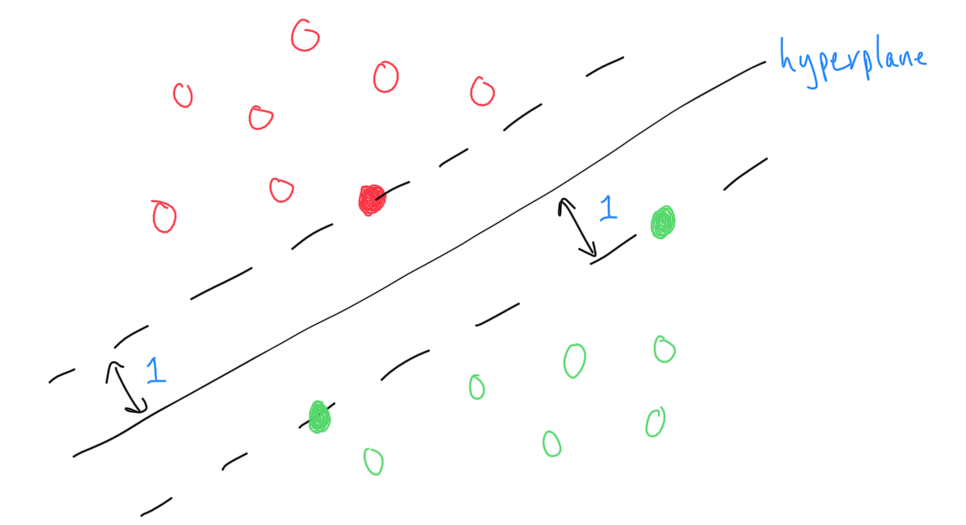
\includegraphics[width=0.5\paperwidth]{old/hard-margin-svm.png}
    \caption{Example of the resulting hyperplane for a hard margin SVM. The filled in data points are
      support vectors in this example. A support vector for the hard-margin formulation must be on the margin boundary, with a discriminant value of +1 or -1.}
    \label{fig:hard-margin-svm}
\end{figure}

\section{Soft Margin Classifier}

Thus far, we've been operating under the assumption that our data is linearly separable in feature space, which afforded us several convenient guarantees in the derivations of the previous section. For example, given that our data was linearly separable, we could guarantee that every data point would be on the correct side of the hyperplane, which waswhat allowed us to enforce the constraint that  $y_{n}(\textbf{w}^\top\textbf{x}_{n} + w_{0}) \geq  1$.
We now seek to generalize the work of the previous section to situations where our data is not
separable.

\subsection{Why the Soft Margin?}

What if our data is not linearly separable in the feature space (even after applying a basis function)?
This is the likely case in real applications!   Unfortunately, our current hard margin SVM formulation would be useless with non-linearly separable data. That is why we need the soft margin SVM.

\begin{figure}
    \centering
    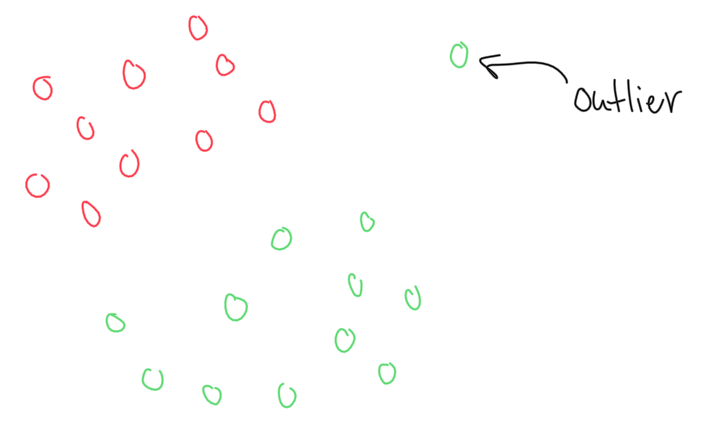
\includegraphics[width=0.5\paperwidth]{old/outlier-data-pt.png}
    \caption{An outlier can make the hard margin formulation impossible or unable to generalize well.}
    \label{fig:outlier-data-pt}
\end{figure}

At a high level, the soft margin SVM allows for some of our data points to be closer to or even on the incorrect side of the hyperplane. This is desirable if our data set is not linearly separable or contains outliers, and it is also quite intuitive. Examining Figure \ref{fig:outlier-data-pt}, we see that we have a single outlier data point. We can still create a good model by just allowing this single data point to be close to the hyperplane (or in some cases, even on the wrong side of the hyperplane). That is what the soft margin formulation will allow for.

\subsection{Updated Optimization Problem for Soft Margins}

To enable the soft margin formulation, we introduce what are known as \textit{slack variables} denoted $\xi_{n} \geq 0$, which simply relax the constraint from Equation \ref{simplified-maximized-margin-optimization} that we imposed in the hard margin formulation.
Say that a data point is ``inside the margin region'' if its discriminant value is in the range $(-1,+1)$.
%
There is a slack variable $\xi_{n} \geq 0$ for every data point $\textbf{x}_{n}$, and they take the following values according to how we classify $\textbf{x}_{n}$:
%
\begin{equation} \label{slack-variable-values}
	\xi_{n} = \begin{cases}
	 	= 0 & \text{if  $\textbf{x}_{n}$  is correctly classified} \\
		\in (0, 1] & \text{if $\textbf{x}_{n}$  is correctly classified but inside the  margin region} \\
		> 1 & \text{if $\textbf{x}_{n}$ is  incorrectly classified} \\
	\end{cases}
      \end{equation}
      
      These slack variable penalize data points on the wrong side of the margin boundary, but they don't forbid us from allowing data points to be on the wrong side if this produces the best model.
      We now reformulate the optimization problem as follows. This is the {\bf soft-margin training problem}:
%
%
      \begin{align} \label{soft-margin-optimization-problem}
  \underset{\textbf{w}, w_{0}}{\min}\ &  \frac{1}{2} ||\textbf{w}||_2^{2} + C \sum_{n=1}^{N} \xi_{n}\\
  \mbox{s.t.}\quad & y_{n}(\textbf{w}^\top\textbf{x}_{n} + w_{0}) \geq 1 - \xi_{n}, \quad \mbox{for all $n$} \notag \\
  &\quad \xi_{n} \geq 0, \quad \mbox{for all $n$}. \notag
\end{align}

Here, $C$ is a regularization parameter that determines how heavily we penalize violations of the hard margin constraints. A large $C$ penalizes violation of the hard margin constraints more heavily, which means our model will follow the data closely and have small regularization. A small $C$ won't heavily penalize having data points inside the margin region, relaxing the constraint and allowing our model to somewhat disregard more of the data. This means more regularization.

\begin{warning}
    Unlike most regularization parameters we've seen thus far, $C$ increases regularization as it gets smaller.
\end{warning}

\subsection{Soft Margin Support Vectors}
Under the the hard margin formulation, the support vectors were some subset of the  data points with $y_{n}(\textbf{w}^\top\textbf{x}_{n} + w_{0})=1$,
and so situated exactly on the margin boundary,  and  they points
closest to the hyperplane.
%Under the soft margin formulation, we no longer have this guarantee since we explicity relaxed it in the name of creating better, more generalizable models.

The support vectors in the soft margin case must be data points that are either  on the margin boundary (and thus $y_{n}(\textbf{w}^\top\textbf{x}_{n} + w_{0})=1$) or for which $\xi_n\in (0,1]$ and in the margin region, or that are misclassified (when $\xi_{n} > 1$). We can visualize this in Figure \ref{fig:soft-margin-svm}.


\begin{warning}
  Not every data point on the margin boundary, in the margin region, or that is misclassified needs to be a support vector in the soft-margin formulation. But those that become support vectors must meet one of these criteria.
\end{warning}
%
\begin{figure}
    \centering
    \textbf{Soft Margin SVM Example}\par\medskip
    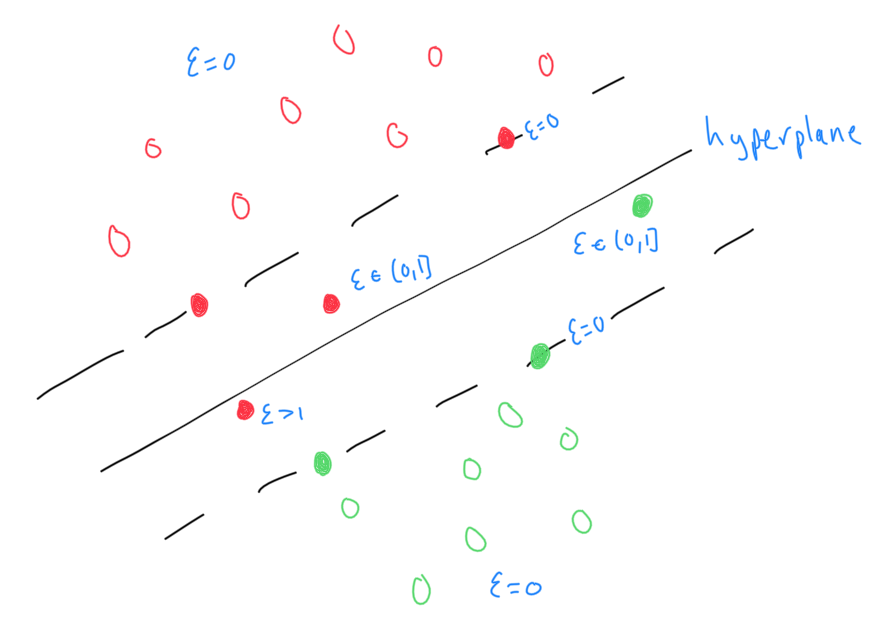
\includegraphics[width=0.5\paperwidth]{old/soft-margin-svm.png}
    \caption{Example of the resulting hyperplane for a soft margin SVM. The filled in data points illustrate the support vectors in this example and must be either on the margin boundary or on the ``wrong side'' of the margin boundary.}
    \label{fig:soft-margin-svm}
\end{figure}

\section{Conversion to Dual Form}

Now that we have the formulation of the optimization problem for SVMs, we need to discuss how we actually go about optimizing to produce a model solution. This will involve converting to a \textit{dual form} of our problem. We will do this in the hard margin case for technical simplicity, but our solution can be easily modified to also  apply to the soft margin formulation.

\begin{warning}
    A dual form is an equivalent manner of representing an optimization problem, in this case the quadratic programming problem we need to optimize. Dual forms can be easier to work with than their initial form (``the primal form.'')
\end{warning}

The dual form will be useful because it will allow us to bring in a basis function into the SVM formulation in a very elegant
and computationally efficient way.

\subsection{Lagrange Multipliers}

Before we get into deriving the dual form, we need to be aware of a critical piece of math that will enable us to solve our optimization problem: \textit{Langrange multipliers}.

A Lagrange multiplier is used to find optima of a function subject to certain constraints. This is exactly what we need to solve the optimization problem described by Equation \ref{final-simplified-maximized-margin-optimization}.

The underlying theory behind Lagrange multipliers is not overly difficult to understand, but it is beyond the scope of this textbook
in its fully generality. We will simply offer the method by which you can use them to solve
the optimization problem of interest here.

Recall from the ``Section 0 math'' that we understood there how to use the  Lagrangian method  to solve optimization problems with equality constraints, for example of the form $\min f(\mathbf{w}) \ \mbox{s.t.}\ g_n(\mathbf{w})=0$, for each constraint $n$. There, a suitable Lagrangian function was $L({\mathbf w},\boldsymbol{\alpha})=f({\mathbf w})+\sum_n\alpha_n g_n(\mathbf{w})$, where $\alpha_n\in\mathbb{R}$ were the Lagrangian variables,
and this problem
could be solved via the partial derivatives of $L$ with respect to ${\mathbf w}$ and $\boldsymbol{\alpha}$, and setting them to zero.
\medskip

Here, we have a slightly different problem to solve, which  has the following form (recognizing that we can write a constraint $ y_{n}(\textbf{w}^\top\textbf{x}_{n} + w_{0}) \geq 1$ as $-y_{n}(\textbf{w}^\top\textbf{x}_{n} + w_{0}) + 1\leq 0$, and thus as an ``$\leq 0$'' constraint):
%
\begin{equation}
  \label{eq:dp1}
  \min_{\mathbf{w}}\ f({\mathbf w}) \quad \mbox{s.t.}\ g_n({\mathbf w})\leq 0, \quad \mbox{all $n$}
\end{equation}

To solve this,  we make use of the same kind of Lagrangian function,
%
\begin{equation}
  \label{eq:dp2}
  L({\mathbf w},\boldsymbol{\alpha})=f({\mathbf w})+\sum_n \alpha_n g_n({\mathbf w}).
\end{equation}

But for the new ``inequality form'' of the constrained optimization problem,
we also need to introduce a new subproblem, which for any fixed ${\mathbf w}$, solves
%
\begin{align}
  \label{eq:dp3}
  \max_{\boldsymbol{\alpha}} L({\mathbf w},\boldsymbol{\alpha}) \quad   \mbox{s.t.} \quad  \alpha_n \geq 0\quad\mbox{for all $n$}
\end{align}

With this, we consider the problem
%
%
\begin{align}
\label{eq:dp4}
 \min_{\mathbf w} \left[\max_{\boldsymbol{\alpha}, \ \boldsymbol{\alpha}\geq 0} f({\mathbf w})+\sum_n \alpha_n g_n({\mathbf w})\right]
\end{align}

Now, if ${\mathbf w}$ violates one or more constraints in~\eqref{eq:dp1}, then the subproblem~\eqref{eq:dp3} becomes unbounded, with $\alpha_n$ on the corresponding constraints driven arbitrarily large. Otherwise, if we have $g_n({\mathbf w})<0$ then we will have $\alpha_n=0$, and
we conclude $\alpha_n g_n({\mathbf x})=0$ in all optimal solutions to~\eqref{eq:dp4}.
 %
Therefore, and assuming that problem~\eqref{eq:dp1} is feasible, we have $L({\mathbf w},\boldsymbol{\alpha})=f({\mathbf w})$ in an optimal solution to~\eqref{eq:dp4}.
%
Thus, we establish that~\eqref{eq:dp4}  is an equivalent formulation  to~\eqref{eq:dp1}.

\medskip

Substituting into our problem~\eqref{final-simplified-maximized-margin-optimization}, the Lagrangian formulation becomes
%
\begin{align}
  \min_{\mathbf{w},w_0}\left[\max_{\boldsymbol{\alpha},\ \boldsymbol{\alpha}\geq 0} \frac{1}{2} {\mathbf w}^\top{\mathbf w} +\sum_n \alpha_n(-y_{n}(\textbf{w}^\top\textbf{x}_{n} + w_{0}) + 1)\right]
\end{align}

Equivalently, it is convenient to write this as
\begin{align}
  \min_{\mathbf{w},w_0}\left[\max_{\boldsymbol{\alpha},\ \boldsymbol{\alpha}\geq 0} \frac{1}{2} {\mathbf w}^\top{\mathbf w} -\sum_n \alpha_n(y_{n}(\textbf{w}^\top\textbf{x}_{n} + w_{0}) - 1)\right],
\end{align}
%
with Lagrangian function
%
\begin{align}
  L({\mathbf w},\boldsymbol{\alpha},w_0)=\frac{1}{2} {\mathbf w}^\top{\mathbf w} -\sum_n \alpha_n(y_{n}(\textbf{w}^\top\textbf{x}_{n} + w_{0}) - 1).
  \end{align}



  \if 0 
If you have a function $f(\textbf{x})$ that you need to optimize (let's say maximization here to be concrete, but minimization applies just the same) subject to the constraint that some function $g(\textbf{x}) = 0$, you can take the following steps. First, construct the Lagrangian function $L(\textbf{x}, \lambda)$:
\begin{equation} \label{lagrangian-fn}
	L(\textbf{x}, \lambda) = f(\textbf{x}) + \lambda g(\textbf{x})
\end{equation}
Then, set the derivative of $L$ with respect to both $\textbf{x}$ and $\lambda$ equal to 0:
\begin{equation*}
	\nabla L_{\textbf{x}} = 0, \qquad \frac{\partial L}{\partial \lambda} = g(\textbf{x}) = 0
\end{equation*}
If $\textbf{x}$ is $D$-dimensional, this will give you a system of $D+1$ equations. You can solve these equations for $\textbf{x}$ to find the optimal value of $f(\textbf{x})$ subject to the constraint $g(\textbf{x})$.

You should also be aware of the case where your constraint $g(\textbf{x})$ is an inequality. If we have $g(\textbf{x}) \geq 0$, we will still have the Lagrangian function given by Equation \ref{lagrangian-fn}. On the other hand, if the inequality constraint is $g(\textbf{x}) \leq 0$, construct your Lagrangian function as follows:
\begin{equation*}
	L(\textbf{x}, \lambda) = f(\textbf{x}) - \lambda g(\textbf{x})
\end{equation*}
where only the sign has changed between the $f(\textbf{x})$ and $g(\textbf{x})$ terms. We will work in the $g(\textbf{x}) \geq 0$ case, which like before we optimize with respect to the parameters $\textbf{x}$ and $\lambda$:
\begin{equation*}
	\nabla L_{\textbf{x}} = 0, \qquad \frac{\partial L}{\partial \lambda} = g(\textbf{x}) \geq 0
\end{equation*}
Regardless of the direction of the inequality, we also now optimize subject to the constraints:
\begin{equation*}
	\qquad \lambda \geq 0, \qquad \lambda g(\textbf{x}) = 0
\end{equation*}

\begin{warning}
    The exact reason for these new constraints when working with inequalities is beyond the scope of this textbook, but it's important to remember that they be met.
\end{warning}

Finally, note that when you are optimizing a function under many constraints, you simply introduce a Lagrange multiplier for each constraint.

\begin{example}{Langrange Multiplier Example}{lagrange-multiplier-example}
	Let's say we had a function $f(\textbf{x})$ we wish to maximize:
	\begin{align*}
		f(\textbf{x}) = x_{1}^{2} + 3x_{2}^{2} + 3
	\end{align*}
	subject to the constraint $g(\textbf{x})$:
	\begin{align*}
		g(\textbf{x}) = 4x_{1} + 4x_{2} - 6 = 0
	\end{align*}
	We begin by construction our Lagrangian function $L(\textbf{x}, \lambda)$:
	\begin{align*}
		L(\textbf{x}, \lambda) = x_{1}^{2} + 3x_{2}^{2} + 3 + \lambda (4x_{1} + 4x_{2} - 6)
	\end{align*}
	We then compute $\nabla L_{\textbf{x}}$ and $\frac{\partial L}{\partial \lambda}$ to get a system of equations:
	\begin{align*}
		2x_{1} + 4\lambda = 0 \\
		6x_{2} + 4\lambda = 0 \\
		4x_{1} + 4x_{2} - 6 = 0
	\end{align*}
	Solving these equations for $x_{1}$, $x_{2}$, and $\lambda$ leaves us with the following mazimized solution:
	\begin{align*}
		(x_{1}^{*}, x_{2}^{*}) = \bigg(\frac{9}{8}, \frac{3}{8}\bigg); \qquad \lambda^{*} = -\frac{9}{16}
	\end{align*}
\end{example}

\fi

\subsection{Deriving the Dual Formulation}

\if 0
Now that we understand Lagrange multipliers and how we can use them for constrained optimization, we can get back to the hard margin SVM optimization problem:
\begin{equation} \label{original-optim-fn}
	\underset{\textbf{w}, w_{0}}{\arg\min} \frac{1}{2} ||\textbf{w}||^{2} \quad \text{s.t.} \quad \forall n \, y_{n}(\textbf{w}^\top\textbf{x}_{n} + w_{0}) \geq 1
\end{equation}
To satisfy these $N$ constraints, we introduce $N$ Lagrange multipliers $\lambda_{0}, ..., \lambda_{N-1} \geq 0$. We then have our Lagrangian function:
\begin{equation} \label{lagrange-equation}
	L(\textbf{w}, w_{0}, \boldsymbol{\lambda}) = \frac{1}{2} ||\textbf{w}||^{2} - \sum_{n=1}^{N} \lambda_{n} (y_{n}(\textbf{w}^\top \textbf{x}_{n} + w_{0}) - 1)
\end{equation}
where $\boldsymbol{\lambda} = \lambda_{0}, ..., \lambda_{N-1}$.

\fi

Using this Lagrangian function, we allow ourselves to switch from solving Equation~\ref{final-simplified-maximized-margin-optimization} to instead solving:
%
\begin{equation} \label{new-optim-fn}
	\underset{\textbf{w}, w_{0}}{\min}\left[ \max_{\boldsymbol{\alpha} , \ \boldsymbol{\alpha} \geq 0} L(\textbf{w},  \boldsymbol{\alpha},w_0)\right]
\end{equation}

\begin{warning}
    The `$\underset{\textbf{w}, w_{0}}{\min} \, \underset{\boldsymbol{\alpha} \geq 0}{\max}$' in Equation \ref{new-optim-fn} may be initially confusing. The way to read this is that for any choice of $\mathbf w$, $w_0$, the inner ``max'' problem then finds values of $\boldsymbol{\alpha}$ to try to ``defeat'' the outer minimization objective.
\end{warning}

We now wish to convert the objective in Equation \ref{new-optim-fn} to a dual objective. Under the sufficient conditions of strong duality which hold for this problem because Equation~\ref{final-simplified-maximized-margin-optimization} has a quadratic objective and linear constraints (but whose explanation is beyond the scope of this textbook), we can equivalently reformulate the optimization problem~\eqref{new-optim-fn} as:
%
%
\begin{equation} \label{dual-objective}
	\max_{\boldsymbol{\alpha}, \ \boldsymbol{\alpha} \geq 0} \left[\underset{\textbf{w}, w_{0}}{\min} L(\textbf{w},  \boldsymbol{\alpha},w_0)\right].
      \end{equation}
      
      At this point, we can use first order optimality conditions to  solve
      for  $\mathbf{w}$, i.e., the inner minimization problem, for some choice of  $\boldsymbol{\alpha}$ values.
      %
      Taking the gradient, setting them equal to 0, and solving for $\textbf{w}$, we have:
      %
\begin{align}
  & \quad \nabla L(\textbf{w},  \boldsymbol{\alpha},w_0)= \textbf{w} - \sum_{n=1}^{N} \alpha_{n} y_{n} \textbf{x}_{n} = 0
  \notag  \\
\Leftrightarrow \quad\quad &	\textbf{w}^{*} = \sum_{n=1}^{N} \alpha_{n} y_{n} \textbf{x}_{n}. \label{solve-for-w}
\end{align}

When we do the same thing for $w_{0}$, we find the following:
\begin{align}
\quad &	\frac{\partial L(\textbf{w},  \boldsymbol{\alpha},w_0)}{\partial w_{0}} = - \sum_{n=1}^{N} \alpha_{n} y_{n} = 0 \notag\\
\Leftrightarrow
\quad\quad & 	\sum_{n=1}^{N} \alpha_{n} y_{n} = 0. \label{solve-for-w0}
        \end{align}

        This is interesting. If $\sum_n \alpha_n y_n< 0$, then $L(\cdot)$ is increasing with $w_0$ without bound, and the inner-minimization would choose $w_0=-\infty$ and this choice of $\boldsymbol{\alpha}$  cannot solve~\eqref{dual-objective}.
        If $\sum_n \alpha_n y_n> 0$, then $L(\cdot)$ is decreasing with $w_0$ without bound, and the inner-minimization would choose $w_0=+\infty$, and this
        choice of $\boldsymbol{\alpha}$ cannot solve~\eqref{dual-objective}.
        We need $\sum_n \alpha_n y_n= 0$ for an optimal solution to~\eqref{dual-objective}.  So, we don't yet obtain the optimal value for $w_0$,
        but we do gain a new constraint on the $\alpha$-values that will need to hold in an optimal solution.
        
        Now we substitute for $\mathbf{w}^*$   into our Lagrangian function, and also assume~\eqref{solve-for-w0},  since this will be adopted as a new constraint in solving the optimization problem.
        Given this, we obtain:
        %
\begin{align} 
          L(\textbf{w}, \boldsymbol{\alpha},w_0) &=
\frac{1}{2}\mathbf{w}^\top \mathbf{w} - \mathbf{w}^\top\sum_n \alpha_ny_n{\mathbf x}_n-w_0\sum_n\alpha_ny_n+\sum_n\alpha_n
  \notag \\
                                                 &=-\frac{1}{2}\mathbf{w}^\top\mathbf{w}+\sum_n\alpha_n\notag \\
                                                 &=\sum_n\alpha_n-\frac{1}{2}\left(\sum_n\alpha_ny_n{\mathbf x}_n\right)^\top\left(\sum_{n'}\alpha_{n'}y_{n'}\mathbf{x}_{n'}\right) \label{plugged-in-lagrangian}
\end{align}
%
where the second equation follows from the first by using~\eqref{solve-for-w} and~\eqref{solve-for-w0}, and the third equation follows by  using~\eqref{solve-for-w}.
%


\if 0


          \frac{1}{2} || \sum_{n=1}^{N} \alpha_{n} y_{n} \textbf{x}_{n} ||^{2} - \sum_{n=1}^{N} \alpha_{n} y_{n} (\sum_{m=1}^{N} \alpha_{m} y_{m} \textbf{x}_{m})^\top \textbf{x}_{n} - \sum_{n=1}^{N} \alpha_{n} y_{n} w_{0} + \sum_{n=1}^{N} \alpha_{n} \\
		= \frac{1}{2} \sum_{n=1}^{N} \sum_{m=1}^{N} \alpha_{n} \alpha_{m} y_{n} y_{m} \textbf{x}_{n}^\top \textbf{x}_{m} - \sum_{n=1}^{N} \sum_{m=1}^{N} \alpha_{n} \alpha_{m} y_{n} y_{m} \textbf{x}_{n}^\top \textbf{x}_{m} - w_{0} \sum_{n=1}^{N} \alpha_{n} y_{n} + \sum_{n=1}^{N} \alpha_{n} \\
		= \sum_{n=1}^{N} \alpha_{n} - \frac{1}{2} \sum_{n=1}^{N} \sum_{m=1}^{N} \alpha_{n} \alpha_{m} y_{n} y_{m} \textbf{x}_{n}^\top \textbf{x}_{m}
	\end{aligned}
      \end{equation}

      \fi

      This is now entirely formulated in terms of $\boldsymbol{\alpha}$, and
      provides the {\bf hard margin, dual formulation}:
      %
      \begin{align}
        \max_{\boldsymbol{\alpha}}\ \ & \sum_n\alpha_n - \frac{1}{2} \sum_{n} \sum_{n'} \alpha_{n} \alpha_{n'} y_{n} y_{n'} \textbf{x}_{n}^\top \textbf{x}_{n'}\\
        \mbox{s.t.}\quad & \sum_n\alpha_n y_n=0, \quad\mbox{for all n}\notag \\
                                      & \alpha_n \geq 0, \quad\mbox{for all n}\notag
                                        \end{align}

                                        Here, we add $ \sum_n\alpha_n y_n=0$ as a constraint.
                                        %
                                        This is another quadratic objective, subject to linear constraints.  This can be solved via SGD or another approach to solving convex optimization problems.
                                        With a little more work we can use the optimal  $\boldsymbol{\alpha}$ values to make predictions.


                                        Although the derivation is out of scope for this textbook, there is also a very similar {\bf dual form for the soft-margin SVM training problem}:
%
                              %
      \begin{align}
        \max_{\boldsymbol{\alpha}}\ \ & \sum_n\alpha_n - \frac{1}{2} \sum_{n} \sum_{n'} \alpha_{n} \alpha_{n'} y_{n} y_{n'} \textbf{x}_{n}^\top \textbf{x}_{n'} \label{eq:dpsoft} \\
        \mbox{s.t.}\quad & \sum_n\alpha_n y_n=0, \quad\mbox{for all n}\notag \\
                                      & C \geq \alpha_n \geq 0, \quad\mbox{for all n}\notag
                                        \end{align}            
                                        
This puts an upper-bound on $\alpha_n$ to prevent the dual from being unbounded in the case where the hard-margin SVM problem is infeasible because the data cannot be separated. 
It is not yet clear why any of this has been useful. We will see the value of the dual formulation when working with basis functions.
                                        
\begin{warning}
    By~\eqref{solve-for-w} we see how to find the weight vector $\mathbf{w}$ from a solution $\boldsymbol{\alpha}$. We didn't yet explain how to find $w_0$. That will be explained next.
\end{warning}
                                        
       

\subsection{Making Predictions}


Substituting the optimal dual solution into the discriminant function, we have
%
\begin{equation} \label{new-classification-fn}
	h(\textbf{x}) = \sum_{n=1}^{N} \alpha_{n} y_{n} \mathbf{x}_{n}^\top \mathbf{x} + w_{0}.
      \end{equation}

      For data points with $\alpha_n>0$, this is taking a weighted vote over examples in the training data based on the size of the inner product $\mathbf{x}^\top_n\mathbf{x}$.
      
Since $\boldsymbol{\alpha}$ are Lagrange multipliers, they are non-negative, and moreover, by reasoning about the ``max subproblem''
      in the min-max formulation~\eqref{eq:dp4}, we know that they take on value zero whenever $y_{n}
      h(\textbf{x}_{n}) > 1$.
%
%
      % which means that for every data point summed in the Equation \ref{new-classification-fn}, we either have that $\alpha_{n} = 0$ or $y_{n} h(\textbf{x}_{n}) = 1$. Any data points where $\alpha_{n} = 0$ don't appear in the summation and thus don't have any impact on the prediction.
      %
  %    
      The data points for which $\alpha_{n} > 0$ are known as \textbf{support vectors}, and
they will  must be data points that are either  on the margin boundary, inside the margin region, or misclassified. For the hard-margin formulation they must be data points on the margin boundary.

This is a major takeaway for the usefulness of SVMs: once we've trained our model, we can discard most of our data. We only need to keep the support vectors to make predictions. Soon we also see the ``kernel trick.'' This also illustrates why we need to solve for the values of $\boldsymbol{\alpha}$: those values dictate which data points are the support vectors for our model.

% Finally, note that the extension of this solution from the hard margin to the soft margin case is straightforward. In fact, the Lagrangian function ends up being identical and we only have a few extra constraints.

\subsection*{Solving for $w_0$}

We can solve for $w_0$ by recognizing that $y_n({\mathbf w}^\top {\mathbf x}_n+w_0)=1$ for any data point on the margin boundary. For the hard-margin formulation we can solve for $w_0$ using any example for which $\alpha_n>0$. For the soft-margin formulation, it can be shown that the only points with $\alpha_n=C$ are those inside the margin region or misclassified, and so that any point with $C>\alpha_n>0$ is on the margin boundary. Any such point can be solved to solve for $w_0$.


\subsection{Why is the Dual Formulation Helpful?}

Beyond having a succinct formulation of the discriminant function (assuming the number of support vectors is small), you might be wondering what exactly we gained by moving to the dual formulation of this problem.

First, the complexity of the optimization problem we're solving changed from one that is dependent on the number of features $D$, i.e., the size of the weight vector, to one that is linearly dependent on the number of data points $N$. Thus, the number of variables to optimize over is now independent of the dimensionality of the feature space.

Second, in the dual formulation, we have the opportunity to take advantage of what's known as the \textit{kernel trick} to map our data $\textbf{x}_{n}$ into higher dimensions without incurring performance costs. This works as follows: notice that the only way in which a feature vector ${\mathbf x}$ is accessed during the training process~\eqref{eq:dpsoft} and at prediction time~\eqref{new-classification-fn} is through the inner product $\textbf{x}^\top\textbf{z}$ between two data points. Suppose that we are using a basis function $\phi: \mathbb{R}^D\to\mathbb{R}^M$, so that this becomes $\phi(\textbf{x})^\top \phi(\textbf{z})$. Now, define {\em kernel function}
%
\begin{equation} \label{kernel-fn}
	K(\textbf{x}, \textbf{z}) = \phi(\textbf{x})^\top \phi(\textbf{z}).
      \end{equation}
      %

      The idea of the kernel trick is that {\em we might be able to compute $K(\cdot,\cdot)$ without actually working in the basis function space, $\mathbb{R}^M$, but rather be able to compute the Kernel function directly through algebra in the lower dimensional space, $\mathbb{R}^D$}.
        %

        For example, it can be shown that the polynomial kernel
        %
        \begin{align}
          K_{\mathrm{poly}}(\mathbf{x},\mathbf{z})=(1+\mathbf{x}^\top \mathbf{z})^q, \quad \mbox{for integers $q\geq 2$}
        \end{align}
        %
        corresponds to computing the inner product with a basis function that makes use of all terms up to degree $q$. When $q=2$, then it is all constant, linear, and quadratic terms. The polynomial kernel function does this without needing to actually project the examples to the higher dimensional space. Rather it takes the inner product in the lower-dimensional space, adds 1 to this scalar, and then raises it to the power of $q$. The implicit basis is growing exponentially large in $q$! 
        
   
\begin{warning}
    The kernel trick can even be used to work in an infinite basis. This is the case with the Gaussian kernel. If that is of interest, you should look into Taylor series basis expansions and the Gaussian kernel.
\end{warning}

The importance of the kernel trick is that when computations can be done efficiently in the initial space $\mathbb{R}^D$, then the training problem can be solved by computing the pairwise $K(\cdot,\cdot)$ values for all pairs of training examples, and then using SGD to solve the dual, soft-margin training problem (with $N$ decision variables).


\subsection{Kernel Composition}

Now that we've seen the usefulness of the kernel trick for working in higher dimensional spaces without incurring performance costs or memory overhead, it's reasonable to wonder what sort of valid kernels we can construct.

To be explicit, by `kernel' we mean a function $K(\textbf{x}, \textbf{z}) = \phi(\textbf{x})^\top \phi(\textbf{z})$ that produces a scalar product from two vectors, as determined by some basis function $\phi$.

Although it is beyond the scope of this textbook, the condition for a kernel function $K(\cdot,\cdot)$ to be valid is that the $N\times N$ matrix $\mathbf{K}$, where element $K_{n,n'}= K(\textbf{x}_{n}, \textbf{x}_{n'})$ should be positive semidefinite for {\em any} choices of the data set $\{ \textbf{x}_{n} \}$. This is known as Mercer's theorem.

\begin{warning}
    The matrix ${\mathbf K}$ of elements $K(\textbf{x}_{n}, \textbf{x}_{n'})$ is known as the \textit{Gram matrix} or \textit{Kernel matrix}.
\end{warning}

In practice,  this provides for a logic for how different valid kernels can be composed (if they maintain a p.s.d.~Gram matrix!). 
%

There exists a set of rules that preserve the validity of kernels through transformations. These include such things as
%
\begin{itemize}
\item scalar multiplication $c \cdot K(\cdot,\cdot)$
\item exponentiation $\exp\{K(\cdot,\cdot)\}$
\item addition $K_{1}(\textbf{x}, \textbf{z}) + K_{2}(\textbf{x}, \textbf{z})$, and
\item multiplication $K_{1}(\textbf{x}, \textbf{z}) \cdot K_{2}(\textbf{x}, \textbf{z})$.
\end{itemize}

It is always possible to test the validity of a given kernel by demonstrating that its Gram matrix $\textbf{K}$ is positive semidefinite.

  % \chapter{Clustering}
In this chapter, we will explore a technique known as clustering. This represents our first foray into unsupervised machine learning techniques. Unlike the previous four chapters, where we explored techniques that assumed a data set of inputs and targets, with the goal of eventually making predictions over unseen data, our data set will no longer contain explicit targets. Instead, these techniques are motivated by the goal of uncovering structure in our data. Identifying clusters of similar data points is a useful and ubiquitous unsupervised technique.

\section{Motivation}
The reasons for using an unsupervised technique like clustering are broad. We often don't have a specific task in mind; rather, we are trying to uncover more information about a potentially opaque data set. For clustering specifically, our unsupervised goal is to group data points that are similar.

There are many reasons why we might separate our data by similarity. For organizational purposes, it's convenient to have different classes of data. It can be easier for a human to sift through data if it's loosely categorized beforehand. It may be a preprocessing step for an inference method; for example, by creating additional features for a supervised technique. It can help identify which features make our data points most distinct from one another. It might even provide some idea of how many distinct data types we have in our set. 

This idea of data being `similar' means that we need some measure of \textit{distance} between our data points. While there are a variety of clustering algorithms available, the importance of this distance measurement is consistent between them.

Distance is meant to capture how `different' two data points are from each other. Then, we can use these distance measurements to determine which data points are similar, and thus should be clustered together. A common distance measurement for two data points $\textbf{x}$ and $\textbf{x}'$ is given by:
\begin{equation} \label{l2-distance}
	|| \textbf{x} - \textbf{x'} ||_{L2} = \sqrt{\sum_{d=1}^{D} (\textbf{x}_{d} - \textbf{x'}_{d})^{2}}
\end{equation}
where $D$ is the dimensionality of our data. This is known as \textbf{L2} or \textbf{Euclidean distance}, and you can likely see the similarity to L2 regularization.

There are a variety of distance measurements available for data points living in a $D$-dimensional Euclidean space, but for other types of data (such as data with discrete features), we would need to select a different distance metric. Furthermore, the metrics we choose to use will have an impact on the final results of our clustering.

\begin{mlcube}[clustering]{Discrete}{Supervised / Unsupervised}{Yes / No}
	In unsupervised learning, the domain refers to the domain of the hidden variable z (which is analogous to y in supervised learning). In clustering, we have z's that represent the discrete clusters. Furthermore, the techniques that we explore in this chapter are fully unsupervised and non-probabilistic.
\end{mlcube}

\subsection{Applications}
Here are a few specific examples of use cases for clustering:

\begin{enumerate}
    \item Determining the number of phenotypes in a population.
    \item Organizing images into folders according to scene similarity.
    \item Grouping financial data as a feature for anticipating extreme market events.
    \item Identifying similar individuals based on DNA sequences.
\end{enumerate}

As we mentioned above, there are different methods available for clustering. In this chapter, we will explore two of the most common techniques: K-Means Clustering and Hierarchical Agglomerative Clustering. We also touch on the flavors available within each of these larger techniques.

\section{K-Means Clustering}
The high level procedure behind K-Means Clustering (known informally as k-means) is as follows:

\begin{enumerate}
    \item Initialize cluster centers by randomly selecting points in our data set.
    \item Using a distance metric of your choosing, assign each data point to the closest cluster.
    \item Update the cluster centers based on your assignments and distance metric (for example, when using L2 distance, we update the cluster centers by averaging the data points assigned to each cluster).
    \item Repeat steps 1 and 2 until convergence.
\end{enumerate}

In the case where we are using the L2 distance metric, this is known as \textit{Lloyd's algorithm}, which we derive in the next section.

\subsection{Lloyd's Algorithm}
Lloyd's algorithm, named after Stuart P. Lloyd who first suggested the algorithm in 1957, optimizes our cluster assignments via a technique known as coordinate descent, which we will learn more about in later chapters.

\begin{derivation}[Lloyd's Algorithm Derivation]
	We begin by defining the objective used by Lloyd's algorithm.

	\underline{\textbf{Objective}}

	The loss function for our current assignment of data points to clusters is given by:
	\begin{equation} \label{clustering-loss-fn}
		\mathcal{L}(\textbf{X}, \big\{\boldsymbol{\mu}\big\}_{c=1}^{C}, \big\{\textbf{r}\big\}_{n=1}^{N}) = \sum_{n=1}^{N} \sum_{c=1}^{C} r_{nc} ||\textbf{x}_{n} - \boldsymbol{\mu}_{c}||_2^{2}
	\end{equation}
	where $\textbf{X}$ is our $N$x$D$ data set ($N$ is the number of data points and $D$ is the dimensionality of our data), $\big\{\boldsymbol{\mu}\big\}_{c=1}^{C}$ is the $C$x$D$ matrix of cluster centers ($C$ is the number of clusters we chose), and $\big\{\textbf{r}\big\}_{n=1}^{N}$ is our $N$x$C$ matrix of \textit{responsibility vectors}. These are one-hot encoded vectors (one per data point), where the 1 is in the position of the cluster to which we assigned the $n$th data point. \newline

	We now define the algorithmic portion of Lloyd's clustering procedure.

	\underline{\textbf{Algorithm}}
	
	We first adjust our responsibility vectors to minimize each data point's distance from its cluster center. Formally:
	\begin{equation} \label{responsibility-vector-update}
		r_{nc} = \begin{cases}
		 	= 1 & \text{if $c = \underset{c'}{\arg\min} ||\textbf{x}_{n} - \boldsymbol{\mu}_{c'}||$} \\
			= 0 & \text{otherwise} \\
		\end{cases}
	\end{equation}
	After updating our responsibility vectors, we now wish to minimize our loss by updating our cluster centers $\boldsymbol{\mu}_{c}$. The cluster centers which minimize our loss can be computed by taking the derivative of our loss with respect to $\boldsymbol{\mu}_{c}$, setting equal to 0, and solving for our new cluster centers $\boldsymbol{\mu}_{c}$:
	\begin{equation} \label{update-cluster-centers}
		\begin{aligned}
			\frac{\partial \mathcal{L}}{\partial \boldsymbol{\mu}_{c}} = -2 \sum_{n=1}^{N} r_{nc} (\textbf{x}_{n} - \boldsymbol{\mu}_{c}) \\
			\boldsymbol{\mu}_{c} = \frac{\sum_{n=1}^{N} r_{nc} \textbf{x}_{n}}{\sum_{n=1}^{N} r_{nc}}
		\end{aligned}
	\end{equation}
	Intuitively, this is the average of all the data points $\textbf{x}_{n}$ assigned to the cluster center $\boldsymbol{\mu}_{c}$.

	We then update our responsibility vectors based on the new cluster centers, update the cluster centers again, and continue this cycle until we have converged on a stable set of cluster centers and responsibility vectors.
\end{derivation}

Note that while Lloyd's algorithm is guaranteed to converge, it is only guaranteed to converge to a locally optimal solution. Finding the globally optimal set of assignments and cluster centers is an NP-hard problem. As a result, a common strategy is to execute Lloyd's algorithm several times with different random initializations of cluster centers, selecting the assignment that minimizes loss across the different trials. Furthermore, to avoid nonsensical solutions due to scale mismatch between features (which would throw our Euclidean distance measurements off), it makes sense to standardize our data in a preprocessing step. This is as easy as subtracting the mean and dividing by the standard deviation across each feature.

\subsection{Example of Lloyd's}
For some more clarity on exactly how Lloyd's algorithm works, let's walk through an example.

\begin{example}{Lloyd's Algorithm Example}{lloyds-algorithm-example}
	We start with a data set of size $N=6$. Each data point is two-dimensional, with each feature taking on a value between -3 and 3. We also have a `Red' and `Green' cluster. Here is a table and graph of our data points, labelled A through F: \newline

	\begin{align*}
		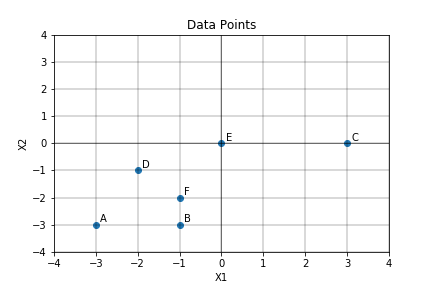
\includegraphics[width=0.5\paperwidth]{old/start-points.png}
	\end{align*}

	\begin{align*}
	\begin{tabular}{lllll}
	\toprule
	{} & Coordinates & Dist. to Red & Dist. to Green & Cluster Assgn. \\
	\midrule
	A &    (-3, -3) &          n/a &            n/a &            n/a \\
	B &    (-1, -3) &          n/a &            n/a &            n/a \\
	C &      (3, 0) &          n/a &            n/a &            n/a \\
	D &    (-2, -1) &          n/a &            n/a &            n/a \\
	E &      (0, 0) &          n/a &            n/a &            n/a \\
	F &    (-1, -2) &          n/a &            n/a &            n/a \\
	\bottomrule
	\end{tabular}
	\end{align*} \newline

	Let's say we wish to have 2 cluster centers. We then randomly initialize those cluster centers by selecting two data points. Let's say we select B and F. We identify our cluster centers with a red and green `X' respectively:

	\begin{align*}
		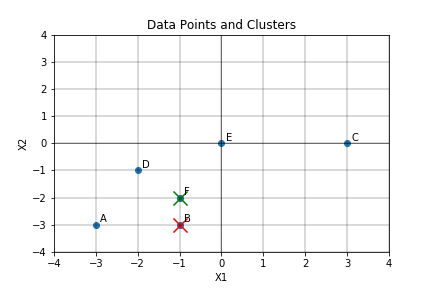
\includegraphics[width=0.5\paperwidth]{old/start-clusters.png}
	\end{align*}

	We now begin Lloyd's algorithm by assigning each data point to its closest cluster center:

	\begin{align*}
		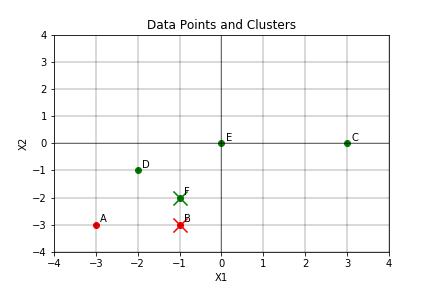
\includegraphics[width=0.5\paperwidth]{old/assign-points.png}
	\end{align*}

	\begin{align*}
	\begin{tabular}{lllll}
	\toprule
	{} & Coordinates & Dist. to Red & Dist. to Green & Cluster Assgn. \\
	\midrule
	A &    (-3, -3) &         n/a &            n/a &              Red \\
	B &    (-1, -3) &         n/a &            n/a &              Red \\
	C &      (3, 0) &         n/a &            n/a &            Green \\
	D &    (-2, -1) &         n/a &            n/a &            Green \\
	E &      (0, 0) &         n/a &            n/a &            Green \\
	F &    (-1, -2) &         n/a &            n/a &            Green \\
	\bottomrule
	\end{tabular}
	\end{align*} \newline

	We then update our cluster centers by averaging the data points assigned to each:

	\begin{align*}
		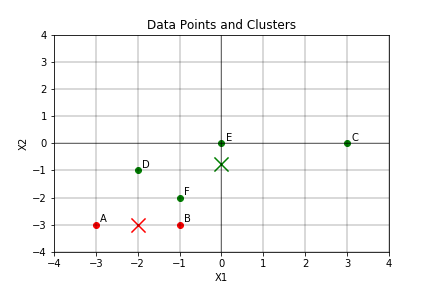
\includegraphics[width=0.5\paperwidth]{old/update-clusters.png}
	\end{align*}

	\begin{align*}
	\begin{tabular}{lllll}
	\toprule
	{} & Coordinates & Dist. to Red & Dist. to Green & Cluster Assgn. \\
	\midrule
	A &    (-3, -3) &         2.00 &           2.24 &            Red \\
	B &    (-1, -3) &         0.00 &           1.00 &            Red \\
	C &      (3, 0) &         5.00 &           4.47 &          Green \\
	D &    (-2, -1) &         2.24 &           1.41 &          Green \\
	E &      (0, 0) &         3.16 &           2.24 &          Green \\
	F &    (-1, -2) &         1.00 &           0.00 &          Green \\
	\bottomrule
	\end{tabular}
	\end{align*}

	We proceed like this, updating our cluster centers and assignments, until convergence. At convergence, we've achieved these cluster centers and assignments:

	\begin{align*}
		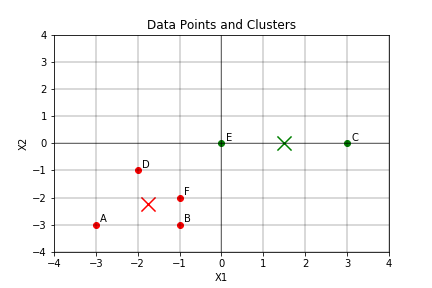
\includegraphics[width=0.5\paperwidth]{old/final-points-and-clusters.png}
	\end{align*}

	\begin{align*}
	\begin{tabular}{lllll}
	\toprule
	{} & Coordinates & Dist. to Red & Dist. to Green & Cluster Assgn. \\
	\midrule
	A &    (-3, -3) &         1.46 &           5.41 &            Red \\
	B &    (-1, -3) &         1.06 &           3.91 &            Red \\
	C &      (3, 0) &         5.26 &           1.50 &          Green \\
	D &    (-2, -1) &         1.27 &           3.64 &            Red \\
	E &      (0, 0) &         2.85 &           1.50 &          Green \\
	F &    (-1, -2) &         0.79 &           3.20 &            Red \\
	\bottomrule
	\end{tabular}
	\end{align*}

	Where our red cluster is at (-1.75, -2.25) and our green cluster is at (1.5 ,  0). Note that for this random initialization of cluster centers, we deterministically identified the locally optimal set of assignments and cluster centers. For a specific initialization, running Lloyd's algorithm will always identify the same set of assignments and cluster centers. However, different initializations will produce different results
\end{example}

\subsection{Number of Clusters}
You may have wondered about a crucial, omitted detail: how do we choose the proper number of clusters for our data set? There doesn't actually exist a `correct' number of clusters. The fewer clusters we have, the larger our loss will be, and as we add more clusters, our loss will get strictly smaller. That being said, there is certainly a tradeoff to be made here.

Having a single cluster is obviously useless - we will group our entire data set into the same cluster. Having $N$ clusters is equally useless - each data point gets its own cluster.

One popular approach to identifying a good number of clusters is to perform K-Means with a varying number of clusters, and then to plot the number of clusters against the loss. Typically, that graph will look like Figure \ref{fig:knee}.

\begin{figure}
    \centering
    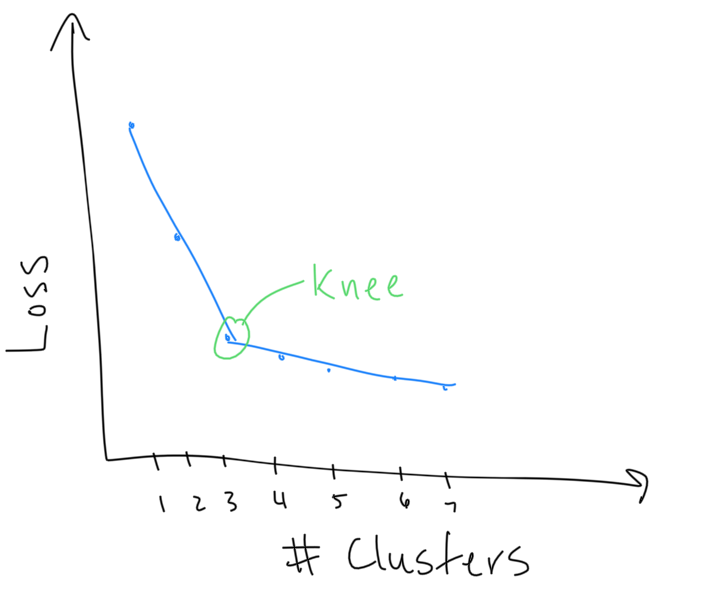
\includegraphics[width=0.5\paperwidth]{old/knee.png}
    \caption{Finding the Knee.}
    \label{fig:knee}
\end{figure}

Notice that at $x=...$ clusters, there appears to be a slight bend in the decrease of our loss. This is often called the \textbf{knee}, and it is common to choose the number of clusters to be where the knee occurs.

Intuitively, the idea here is that up to a certain point, adding another cluster significantly decreases the loss by more properly grouping our data points. However, eventually the benefit of adding another cluster stops being quite so significant. At this point, we have identified a natural number of groups for our data set.

\subsection{Initialization and K-Means++}
Up until now, we have assumed that we should randomly initialize our cluster centers and execute Lloyd's algorithm until convergence. We also suggested that since Lloyd's algorithm only produces a local minimum, it makes sense to perform several random initializations before settling on the most optimal assignment we've identified.

While this is a viable way to perform K-Means, there are other ways of initializing our original cluster centers that can help us find more optimal results without needing so many random initializations. One of those techniques is known as \textbf{K-Means++}.

The idea behind K-Means++ is that our cluster centers will typically be spread out when we've reached convergence. As a result, it might not make sense to initialize those cluster centers in an entirely random manner. For example, Figure \ref{fig:bad-init} would be a poor initialization.

\begin{figure}
    \centering
    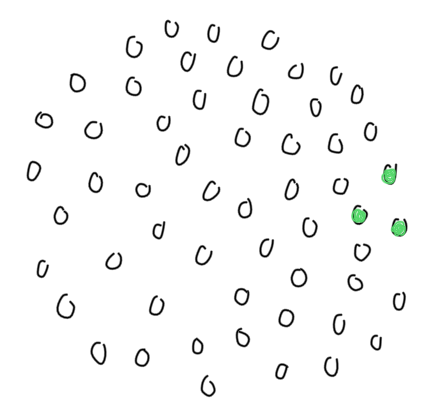
\includegraphics[width=0.5\paperwidth]{old/bad-initialization.png}
    \caption{Bad Cluster Initialization.}
    \label{fig:bad-init}
\end{figure}

We would much rather start with a random initialization that looks like Figure \ref{fig:good-init}.

\begin{figure}
    \centering
    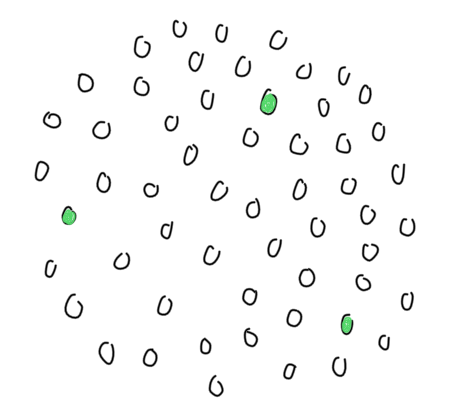
\includegraphics[width=0.5\paperwidth]{old/good-initialization.png}
    \caption{Good Cluster Initialization.}
    \label{fig:good-init}
\end{figure}

We can use the hint that we want our cluster centers somewhat spread out to find a better random initialization. This is where the initialization algorithm presented by K-Means++ comes in.

For K-Means++, we choose the first cluster center by randomly selecting a point in our data set, same as before. However, for all subsequent cluster center initializations, we select points in our data set with probability proportional to the squared distance from their nearest cluster center. The effect of this is that we end up with a set of initializations that are relatively far from one another, as in Figure \ref{fig:good-init}.

\subsection{K-Medoids Alternative}
Recall that in the cluster center update step (Equation \ref{update-cluster-centers}) presented in the derivation of Lloyd's algorithm, we average the data points assigned to each cluster to compute the new cluster centers. Note that in some cases, this averaging step doesn't actually make sense (for example, if we have categorical variables as part of our feature set). In these cases, we can use an alternative algorithm known as \textbf{K-Medoids}. The idea behind K-Medoids is simple: instead of averaging the data points assigned to that cluster, update the new cluster center to be the data point assigned to that cluster which is most like the others.

\section{Hierarchical Agglomerative Clustering}
The motivating idea behind K-Means was that we could use a distance measurement to assign data points to a fixed number of clusters, iteratively improving our assignments and cluster locations until convergence.

Moving on to Hierarchical Agglomerative Clustering (also known as \textbf{HAC} - pronounced `hack'), the motivating idea is instead to group data from the bottom up. This means every data point starts as its own cluster, and then we merge clusters together based on a distance metric that we define. This iterative merging allows us to construct a tree over our data set that describes relationships between our data. These trees are known as \textit{dendrograms}, with an example found in Figure \ref{fig:dendrogram-example}. Notice that the individual data points are the leaves of our tree, and the trunk is the cluster that contains the entirety of our data set.

\begin{figure}
    \centering
    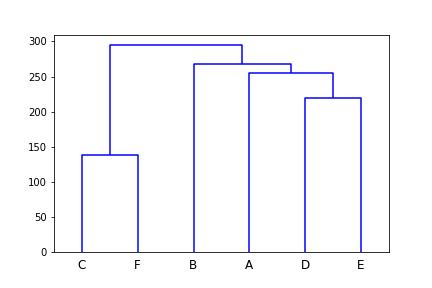
\includegraphics[width=0.5\paperwidth]{old/dendrogram-example.png}
    \caption{Dendrogram Example.}
    \label{fig:dendrogram-example}
\end{figure}

We now formally define the HAC algorithm, and in the process, explain how we construct such a tree.

\subsection{HAC Algorithm}
\begin{enumerate}
    \item Start with $N$ clusters, one for each data point.
    \item Measure the distance between clusters. This will require an inter-cluster distance measurement that we will define shortly.
    \item Merge the two `closest' clusters together, reducing the number of clusters by 1. Record the distance between these two merged clusters.
    \item Repeat step 2 until we're left with only a single cluster.
\end{enumerate}

In the remainder of the chapter, we'll describe this procedure in greater detail (including how to measure the distance between clusters), explain the clustering information produced by the tree, and discuss how HAC differs from K-Means. But first, to make this algorithm a little more clear, let's perform HAC one step at a time on a toy data set, constructing the dendrogram as we go.

\begin{example}{HAC Algorithm Example}{hac-algo-example}
Let's say we have a data set of five points A, B, C, D, E that we wish to perform HAC on. These points will simply be scalar data that we can represent on a number line. We start with 5 clusters and no connections at all:

\begin{align*}
	
\includegraphics[width=0.5\paperwidth]{old/number-line.png}
\end{align*}

We find the closest two clusters to merge first. A and B are nearest (it's actually tied with C and D, but we can arbitrarily break these ties), so we start by merging them. Notice that we also annotate the distance between them in the tree, which in this case is 1:

\begin{align*}
	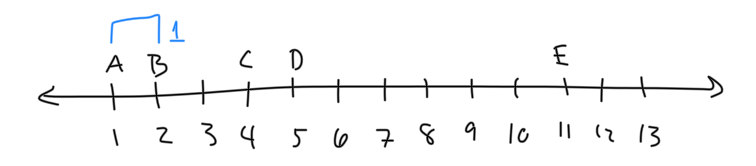
\includegraphics[width=0.5\paperwidth]{old/a-b-merged.png}
\end{align*}

We now have four clusters: (A, B), C, D, and E. We again find the closest two clusters, which in this case is C and D:

\begin{align*}
	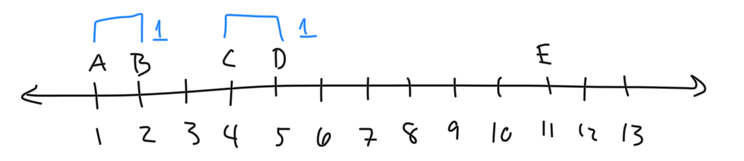
\includegraphics[width=0.5\paperwidth]{old/c-d-merged.png}
\end{align*}

We now have three remaining clusters: (A, B), (C, D), and E. We proceed as before, identifying the two closest clusters to be (A, B) and (C, D). Merging them:

\begin{align*}
	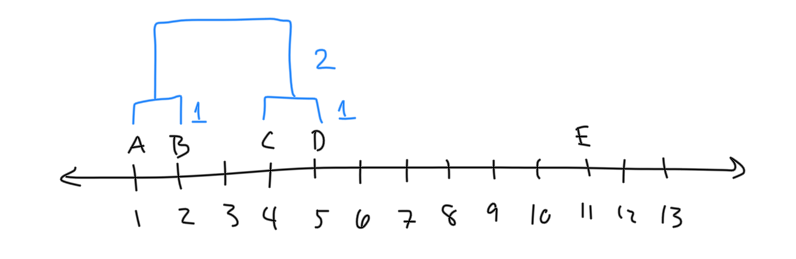
\includegraphics[width=0.5\paperwidth]{old/a-b-c-d-merged.png}
\end{align*}

Finally we are left with two clusters: (A, B, C, D) and E. The remaining two clusters are obviously the closest together, so we merge them:

\begin{align*}
	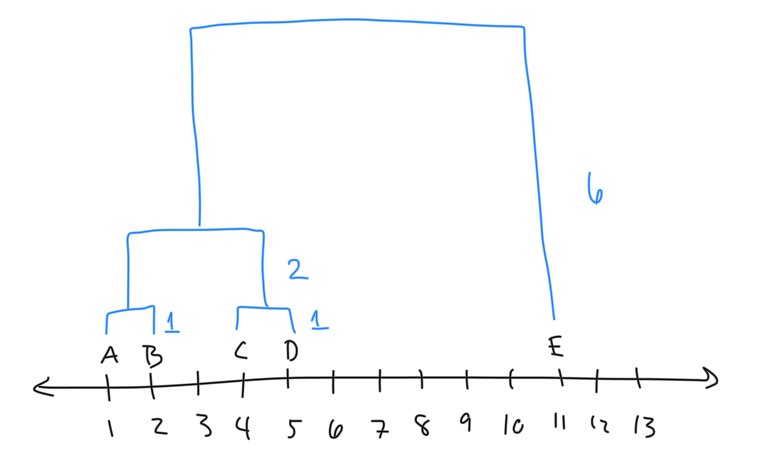
\includegraphics[width=0.5\paperwidth]{old/a-b-c-d-e-merged.png}
\end{align*}

At this point there is only a single cluster. We have constructed our tree and are finished with HAC.
\end{example}

Notice how the distance between two merged clusters manifests itself through the height of the dendrogram where they merge (which is why we tracked those distances as we constructed the tree). Notice also that we now have many layers of clustering: if we're only only interested in clusters whose elements are at least $k$ units away from each other, we can `cut' the dendrogram at that height and examine all the clusters that exist below that cut point.

Finally, we need to handle the important detail of how to compute the distance between clusters. In the preceding example, we designated the distance between two clusters to be the minimum distance between any two data points in the clusters. This is what is known as the \textbf{Min-Linkage Criterion}. However, there are certainly other ways we could have computed the distance between clusters, and using a different distance measurement can produce different clustering results. We now turn to these different methods and the properties of clusters they produce.

\subsection{Linkage Criterion}
Here are a few of the most common linkage criteria.

\subsubsection{Min-Linkage Criteria}
We've already seen the Min-Linkage Criterion in action from the previous example. Formally, the criterion says that the distance $d_{C, C'}$ between each cluster pair $C$ and $C'$ is given by
\begin{equation} \label{min-linkage-crit}
	d_{C, C'} = \underset{k, k'}{\min} || \textbf{x}_{k} - \textbf{x}_{k'} ||
\end{equation}
where $\textbf{x}_{k}$ are data points in cluster $C$ and $\textbf{x}_{k'}$ are data points in cluster $C'$. After computing these pairwise distances, we choose to merge the two clusters that are closest together.

\subsubsection{Max-Linkage Criterion}
We could also imagine defining the distance $d_{C, C'}$ between two clusters as being the distance between the two points that are farthest apart in each cluster. This is known as the Max-Linkage Criterion. The distance between two clusters is then given by:
\begin{equation} \label{max-linkage-crit}
	d_{C, C'} = \underset{k, k'}{\max} || \textbf{x}_{k} - \textbf{x}_{k'} ||
\end{equation}
As with the Min-Linkage Criterion, after computing these pairwise distances, we choose to merge the two clusters that are closest together.

\begin{warning}
    Be careful not to confuse the linkage criterion with which clusters we choose to merge. We \textbf{always} merge the clusters that have the smallest distance between them. How we compute that distance is given by the linkage criterion.
\end{warning}

\subsubsection{Average-Linkage Criterion}
The Average-Linkage Criterion averages the pairwise distance between each point in each cluster. Formally, this is given by:
\begin{equation} \label{avg-linkage-crit}
	d_{C, C'} = \frac{1}{K K'} \sum_{k=1}^{K} \sum_{k'=1}^{K'} || \textbf{x}_{k} - \textbf{x}_{k'} ||
\end{equation}

\subsubsection{Centroid-Linkage Criterion}
The Centroid-Linkage Criterion uses the distance between the centroid of each cluster (which is the average of the data points in a cluster). Formally, this is given by:
\begin{equation} \label{cent-linkage-crit}
	d_{C, C'} = || \frac{1}{K} \sum_{k=1}^{K} \textbf{x}_{k} - \frac{1}{K'} \sum_{k'=1}^{K'} \textbf{x}_{k'} ||
\end{equation}

\subsubsection{Different Linkage Criteria Produce Different Clusterings}
It's important to note that the linkage criterion you choose to use will influence your final clustering results. For example, the min-linkage criterion tends to produce `stringy' clusters, while the max-linkage criterion tends to produce more compact clusters. You can see the difference between the results of these two linkage criteria in Figure \ref{fig:diff-linkage-criteria}.

\begin{figure}
    \centering
    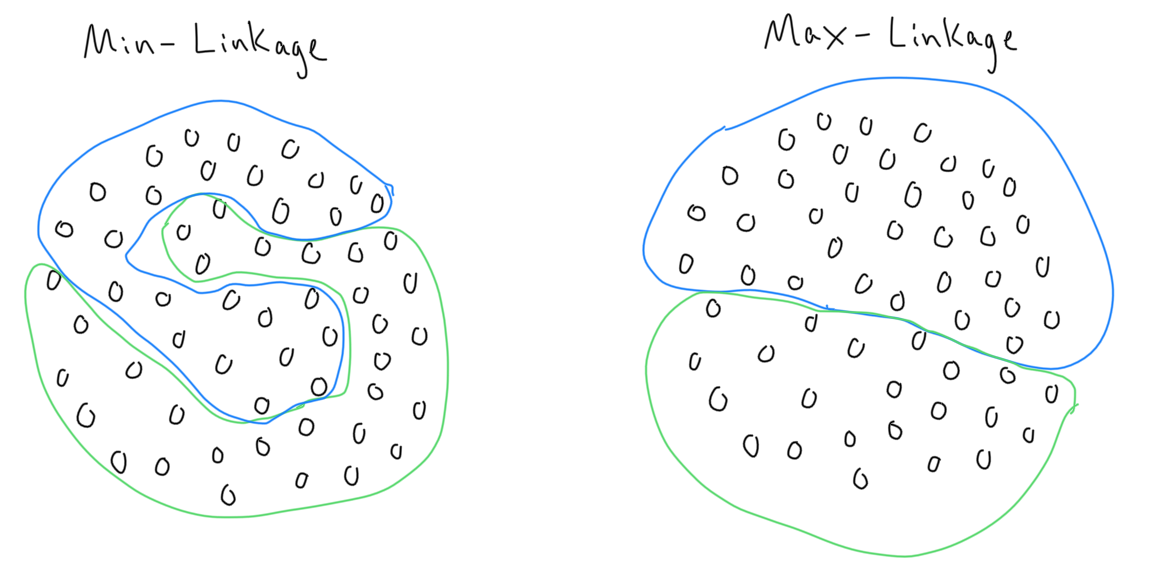
\includegraphics[width=0.5\paperwidth]{old/diff-linkage-criteria.png}
    \caption{Different Linkage Criteria.}
    \label{fig:diff-linkage-criteria}
\end{figure}

\begin{warning}
    You should convince yourself of the different flavors of linkage criteria. For example, when using the min-linkage criterion, we get these `stringy' results because we're most inclined to extend existing clusters by grabbing whichever data points are closest.
\end{warning}

\subsection{How HAC Differs from K-Means}
Now that we're aware of two distinct clustering techniques and their variants, we consider the differences between the two methods.

First of all, there is a fundamental difference in determinism between HAC and K-Means. In general, K-Means incurs a certain amount of randomness and needs to be run multiple times to ensure a good result. On the other hand, once you've selected a linkage criterion for HAC, the clusters you calculate are deterministic. You only need to run HAC a single time.

Another difference between HAC and K-Means comes from the assumptions we make. For K-Means, we need to specify the number of clusters up front before running our algorithm, potentially using something like the knee-method to decide on the number of clusters. On the other hand, you don't need to assume anything to run HAC, which simplifies its usage. However, the downside for HAC is that when you wish to present your final clustering results, you need to decide on the max distance between elements in each cluster (so that you can cut the dendrogram).

The fact that you need to make a decision about where to cut the dendrogram means that running HAC once gives you several different clustering options. Furthermore, the dendrogram in and of itself can be a useful tool for visualizing data. We don't get the same interactivity from K-Means clustering.

\begin{warning}
    We often use dendrograms to visualize evolutionary lineage.
\end{warning}
  % \chapter{Dimensionality Reduction}
In previous chapters covering supervised learning techniques, we often used basis functions to project our data into higher dimensions prior to applying an inference technique. This allowed us to construct more expressive models, which ultimately produced better results. While it may seem counterintuitive, in this chapter we're going to focus on doing exactly the opposite: reducing the dimensionality of our data through a technique known as Principal Component Analysis (PCA). We will also explore why it is useful to reduce the dimensionality of some data sets.

\section{Motivation}
Real-world data is often very high dimensional, and it's common that our data sets contain information we are unfamiliar with because the dimensionality is too large for us to comb through all the features the by hand.

In these situations, it can be very difficult to manipulate or utilize our data effectively. We don't have a sense for which features are `important' and which ones are just noise. Fitting a model to the data may be computationally expensive, and even if we were to fit some sort of model to our data, it may be difficult to interpret why we obtain specific results. It's also hard to gain intuition about our data through visualization since humans struggle to think in more than three dimensions. All of these are good reasons that we may wish to reduce the dimensionality of a data set.

\begin{mlcube}{Dimensionality Reduction}
Dimensionality reduction operates primarily on continuous feature spaces, is fully unsupervised, and is non-probabilistic for the techniques we explore in this chapter.
\begin{center}
    \begin{tabular}{c|c|c}
    \textit{\textbf{Domain}} & \textit{\textbf{Training}} & \textit{\textbf{Probabilistic}} \\
    \hline
    Continuous & Unsupervised & No \\
    \end{tabular}
\end{center}
\end{mlcube}

While dimensionality reduction is considered an unsupervised technique, it might also be thought of as a tool used to make data more manageable prior to taking some other action. In fact, it's an important preprocessing step for a host of use cases.

\section{Applications}
As described above, we need a tool like dimensionality reduction in situations where high-dimensional data hinders us. Here are a few specific situations where we would use such a technique:

\begin{enumerate}
    \item Presenting differences between complex molecules in two dimensions (via a graph).
    \item Understanding the results of a credit trustworthiness algorithm.
    \item Efficiently training a neural network to predict supermarket sales on a data set with many input features.
    \item Identifying which costly measurements are worth collecting when experimenting with new chemicals.
\end{enumerate}

With a few of these use cases in mind, we now turn to the math that underpins the dimensionality reduction technique known as Priniciple Component Analysis.

\section{Principal Component Analysis}
The main idea behind Principal Component Analysis (PCA) is that we can linearly project our data set onto a subspace without losing too much information. For example, three-dimensional data might primarily exist in a subspace that is actually a two-dimensional plane.

One way to think about this is to identify and preserve the features along which there is the most variance. For example, imagine we had a data set comprised of the heights and weights of individual bears. As an extreme case, let's suppose all the bears were exactly the same height but had a wide range of weights.

\begin{figure}
    \centering
    \textbf{Bear Heights and Weights}\par\medskip
    
\includegraphics[width=0.5\paperwidth]{old/bear-graph.png}
    \caption{Graph of bear heights and weights.}
    \label{fig:bear-graph}
\end{figure}

To differentiate our data points, we obviously only need to report the weights of the bears. The variance of the heights is 0, and the variance of the weights is some non-zero number. Intuitively, the most interesting features from our data sets are those that vary the most.

\begin{warning}
    In this simple example, the direction of maximal variance occurs exactly along the $x_1$ axis, but in general it will occur on a plane described by a combination of our input features.
\end{warning}

The second way to think about PCA is that we are minimizing the error we incur when we move from the lower-dimensional representation back to the original representation. This is known as \textit{reconstruction loss}. We can consider the meaning of this using our bear example.

Let's say we project the data set from Figure \ref{fig:bear-graph} here down to a single dimension by recording only the weights:

\begin{figure}
    \centering
    \textbf{Bear Weights}\par\medskip
    
\includegraphics[width=0.5\paperwidth]{old/bear-weights-line.png}
    \caption{Bear weights.}
    \label{fig:bear-weights-line}
\end{figure}

Then, to reconstruct our original graph, we need only to keep track of a slope and bias term in the form of the familiar equation $x_2 = mx_1 + b$. In this case our slope is $m=0$ and our bias $b=3$. Note that this storage overhead is constant (just remembering the slope and bias) regardless of how big our data set gets. Thus we can go from our low-dimensional representation back to our original data:

\begin{figure}
    \centering
    \textbf{Converting Between Reduced and Original Data}\par\medskip
    \includegraphics[width=0.5\paperwidth]{old/bear-conversion.png}
    \caption{Converting between the reduced data and original data.}
    \label{fig:bear-conversion}
\end{figure}

It will be our goal to determine a low-dimensional representation of our data that allows us to return to our high-dimensional data while losing as little information as possible. We wish to preserve everything salient about the data while discarding as much redundant information as possible. We now turn to how this can be achieved.

\subsection{Reconstruction Loss}
We identified a key tenet of dimensionality reduction in the previous section: finding subspaces of our data that preserve as much information as possible. Concretely, this means we want to convert our original data point $\textbf{x}_n$ in $D$ dimensions into a data point $\textbf{x}'_{n}$ in $D'$ dimensions where $D' < D$.

\begin{warning}
    We're going to assume that our data set has been mean-centered such that each feature in $\textbf{x}_{n}$ has mean 0. This will not affect the application of the method (we can always convert back to the uncentered data by adding back the mean of each feature), but will make our derivations more convenient to work with.
\end{warning}


Let's consider a simple case first: $D'=1$. This means that we're projecting our $D$ dimensional data down onto just a single dimension, or in geometric terms, we're projecting our data points $\textbf{x}_{n}$ onto a line through the origin. We can define this line as the unit vector $\textbf{w} \in \mathbb{R}^{D \times 1}$, and the projection is given by the dot product $\textbf{x} \cdot \textbf{w}$.

\begin{warning}
    The unit vector $\textbf{w}$ onto which we project our data is known as a \textit{principal component}, from which PCA gets its name.
\end{warning}

This projection produces a scalar, and that scalar defines how far our projection $\textbf{x} \cdot \textbf{w}$ is from the origin. We can convert this scalar back to $D$ dimensional space by multiplying it with the unit vector $\textbf{w}$. This means that $(\textbf{x} \cdot \textbf{w})\textbf{w}$ is the result of projecting our data point $\textbf{x}$ down into one-dimension and then converting it to its coordinate location in $D$ dimensions. We refer to these as our \textit{projection vectors}, and we can observe what this looks like geometrically in Figure \ref{fig:data-reconstruction}.

\begin{figure}
    \centering
    \textbf{Data Reconstruction}\par\medskip
    \includegraphics[width=0.5\paperwidth]{old/data-reconstruction.png}
    \caption{Far left: our original data. Middle: our reduced data in scalar form after the projection given by $\textbf{x} \cdot \textbf{w}$. Right: our reconstructed data points given by $(\textbf{x} \cdot \textbf{w})\textbf{w}$. Notice that our reconstructed data points are not the same as our original data.}
    \label{fig:data-reconstruction}
\end{figure}

The projection vectors we recover from the expression $(\textbf{x} \cdot \textbf{w})\textbf{w}$ will be in $D$ dimensions, but they will obviously not be identical to the original $D$ dimensional vectors (Figure \ref{fig:data-reconstruction} demonstrates why that is the case). This difference between the original and projection vectors can be thought of as error, since it is information lost from our original data. For a given data point $\textbf{x}_{n}$ and unit vector $\textbf{w}$, we can measure this error through the expression:
\begin{equation} \label{reconstruction-loss}
	||\textbf{x}_{n} - (\textbf{x} \cdot \textbf{w})\textbf{w}||^{2}
\end{equation}
which is known as \textbf{reconstruction loss} because it measures the error incurred when reconstructing our original data from its projection.

\begin{definition}[reconstruction loss]
    Reconstruction loss is the difference (measured via a distance metric such as Euclidean distance) between an original data set and its reconstruction from a lower dimensional representation. It indicates how much information is lost during dimensionality reduction.
\end{definition}

Reconstruction loss is then a metric for evaluating how `good' a subspace in $D'$ dimensions is at representing our original data in $D$ dimensions. The better it is, the less information we lose, and the reconstruction loss is lower as a result.

\subsection{Minimizing Reconstruction Loss}
We now know that our goal is to find a good subspace to project onto, and we also know that finding this good subspace is equivalent to minimizing the reconstruction loss it incurs. We can now formalize this as an optimization problem.

First, we simplify the reconstruction loss for a single data point $\textbf{x}_n$ as follows:
\begin{align*}
	||\textbf{x}_{n} - (\textbf{x}_{n} \cdot \textbf{w})\textbf{w}||^{2} &= (\textbf{x}_{n} - (\textbf{x}_{n} \cdot \textbf{w})\textbf{w})(\textbf{x}_{n} - (\textbf{x}_{n} \cdot \textbf{w})\textbf{w}) \\
	&= ||\textbf{x}_{n}||^{2} - 2(\textbf{x}_{n} \cdot \textbf{w})^{2} + (\textbf{x}_{n} \cdot \textbf{w})^{2}||\textbf{w}||^{2} \\
	&= ||\textbf{x}_{n}||^{2} - (\textbf{x}_{n} \cdot \textbf{w})^{2} \\
\end{align*}
where $||\textbf{w}||^{2} = 1$ because it is a unit vector. Note that we can define reconstruction loss over our entire data set as follows:
\begin{equation} \label{full-reconstruction-loss}
    RL(\textbf{w}) = \frac{1}{N} \sum_{n=1}^{N} ||\textbf{x}_{n}||^{2} - (\textbf{x}_{n} \cdot \textbf{w})^{2} \\
\end{equation}
Recall that our goal is to minimize reconstruction loss over our data set by optimizing the subspace defined by $\textbf{w}$. Let's first rewrite Equation \ref{full-reconstruction-loss} as:
\begin{align*}
    RL(\textbf{w}) = \frac{1}{N} \sum_{n=1}^{N} ||\textbf{x}_{n}||^{2} - \frac{1}{M} \sum_{n=1}^{N} (\textbf{x}_{n} \cdot \textbf{w})^{2} \\
\end{align*}
where we can see that our optimization will depend only on maximizing the second term:
\begin{equation} \label{max-for-recon-loss}
    \max_{\textbf{w}} \frac{1}{N} \sum_{n=1}^{N} (\textbf{x}_{n} \cdot \textbf{w})^{2}
\end{equation}
since it is the only one involving \textbf{w}. Recall that the sample mean of a data set is given by the expression $\frac{1}{N} \sum_{n=1}^{N} \textbf{x}_{n}$, and note that Equation \ref{max-for-recon-loss} is the sample mean of $(\textbf{x} \cdot \textbf{w})^{2}$. Using the definition of variance for a random variable $\textbf{Z}$ (which is given by $Var(\textbf{Z}) = \mathbb{E}(\textbf{Z}^{2}) - (\mathbb{E}(\textbf{Z}))^{2}$), we can rewrite Equation \ref{max-for-recon-loss} as:
\begin{align*}
    \frac{1}{N} \sum_{n=1}^{N} (\textbf{x}_{n} \cdot \textbf{w})^{2} &= Var\big[\{\textbf{x}_{n} \cdot \textbf{w}\}_{n=1}^{N}\big] + \big( \mathbb{E} \big[\{\textbf{x}_{n} \cdot \textbf{w}\}_{n=1}^{N}\big] \big)^{2}
\end{align*}
Recall that we centered our data $\textbf{x}_{n}$ to have mean 0 such that the expression above simplifies to:
\begin{equation} \label{variance-equivalence}
    \frac{1}{N} \sum_{n=1}^{N} (\textbf{x}_{n} \cdot \textbf{w})^{2} = Var\big[\{\textbf{x}_{n} \cdot \textbf{w}\}_{n=1}^{N}\big] \\
\end{equation}
and therefore $Var\big[\{\textbf{x}_{n} \cdot \textbf{w}\}_{n=1}^{N}\big]$ is the term we wish to maximize. \textbf{This means that minimizing the reconstruction loss is equivalent to maximizing the variance of our projections $\{\textbf{x}_{n} \cdot \textbf{w}\}_{n=1}^{N}$}.

\begin{warning}
    Note the intuitiveness of this result. We should like to find a subspace that maintains the spread in our data.
\end{warning}

\subsection{Multiple Principal Components}
Up until now, we've been considering how we would project onto a single principal component $\textbf{w} \in \mathbb{R}^{D \times 1}$. This will reduce our data down to one dimension, just a scalar. In general, we will wish to preserve more of our data than just a single dimension (in order to capture more of the variance in our data and reduce reconstruction loss), which means that we will need to have multiple principal components. For now we'll assume that our principal components are orthogonal (we will prove this later), which then allows us to describe the projection of our data $\textbf{x}_{n}$ onto this subspace as the sum of the projections onto $D'$ orthogonal vectors:
\begin{equation} \label{orthogonal-projections}
    \sum_{d'=1}^{D'} (\textbf{x}_{n} \cdot \textbf{w}_{d'})\textbf{w}_{d'}
\end{equation}

\subsection{Identifying Directions of Maximal Variance in our Data}
We now know from the previous section that we find our principal components (and thus the subspace we will project onto) by identifying the directions of maximum variance in our projected data set. We know from Equation \ref{variance-equivalence} that the variance is equivalent to:
\begin{equation*}
    \sigma^{2}_{\textbf{w}} \equiv Var\big[\{\textbf{x}_{n} \cdot \textbf{w}\}_{n=1}^{N}\big] = \frac{1}{N} \sum_{n=1}^{N} (\textbf{x}_{n} \cdot \textbf{w})^{2}
\end{equation*}
Rewriting this in terms of matrix notation we have that:
\begin{equation*}
    \sigma^{2}_{\textbf{w}} = \frac{1}{N} (\textbf{X} \textbf{w})^{T} (\textbf{X} \textbf{w})
\end{equation*}
We can further simplify this:
\begin{align*}
    \sigma^{2}_{\textbf{w}} &= \frac{1}{N} \textbf{w}^{T}\textbf{X}^{T} \textbf{X} \textbf{w} \\
    \sigma^{2}_{\textbf{w}} &= \textbf{w}^{T} \frac{\textbf{X}^{T}\textbf{X}}{N} \textbf{w} \\
    \sigma^{2}_{\textbf{w}} &= \textbf{w}^{T} \textbf{S} \textbf{w} \\
\end{align*}
where, since we assume the design matrix $\mathbf{X}$ is {\bf mean-centered}, then  $\textbf{S} = \frac{\textbf{X}^{T}\textbf{X}}{N}$ is the empirical covariance matrix of our data set.

\begin{warning}
    Notice that by convention we describe the empirical covariance of a data set with the term $\textbf{S}$ instead of the usual covariance term $\Sigma$.
\end{warning}

Our goal is to maximize the term $\sigma^{2}_{\textbf{w}} = Var\big[\{\textbf{x}_{n} \cdot \textbf{w}\}_{n=1}^{N}\big]$ with respect to $\textbf{w}$. Furthermore, $\textbf{w}$ is a unit vector, so we must optimize subject to the constraint $\textbf{w}^{T}\textbf{w} = 1$. Recalling the discussion of Lagrange multipliers from Chapter 6 on Support Vector Machines, we incorporate this constraint by reformulating our optimization problem as the Lagrangian equation:
\begin{align*}
    \mathcal{L}(\textbf{w}, \lambda) &= \textbf{w}^{T} \textbf{S} \textbf{w} - \lambda(\textbf{w}^{T}\textbf{w} - 1) \\
\end{align*}
As usual, we proceed by taking the derivative with respect to each parameter:
\begin{align*}
    \frac{d\mathcal{L}(\textbf{w}, \lambda)}{d\textbf{w}} &= 2\textbf{S} \textbf{w} - 2\lambda\textbf{w} \\
    \frac{d\mathcal{L}(\textbf{w}, \lambda)}{d\lambda} &= \textbf{w}^{T}\textbf{w} - 1 \\
\end{align*}
We can now set these equal to 0 and solve for the optimal values:
\begin{align*}
    \textbf{S} \textbf{w} &= \lambda\textbf{w} \\
    \textbf{w}^{T}\textbf{w} &= 1 \\
\end{align*}
This result is very significant! As we knew already, we needed $\textbf{w}$ to be a unit vector. However, we also see that $\textbf{w}$ is an eigenvector of the empirical covariance matrix $\textbf{w}$. Futhermore, the eigenvector that will maximize our quantity of interest $\sigma^{2}_{\textbf{w}} = \textbf{w}^{T} \textbf{S} \textbf{w}$ will be the eigenvector with the largest eigenvalue $\lambda$.

Linear algebra gives us many tools for finding eigenvectors, and as a result we can efficiently identify our principal components. Note also that the eigenvectors of a symmetric matrix are orthogonal, which proves our earlier assumption that our principal components are orthogonal.

\begin{warning}
    Each eigenvector is a principal component. The larger the eigenvalue associated with that principal component, the more variance there is along that principal component.
\end{warning}

To recap, we've learned that the optimal principal components (meaning the vectors describing our projection subspace) are the eigenvectors of the empirical covariance matrix of our data set. The vector preserving the most variance in our data (and thus minimizing the reconstruction loss) is given by the eigenvector with the largest eigenvalue, followed by the eigenvector with the next largest eigenvalue, and so on. Furthermore, while it is somewhat outside the scope of this textbook, we are guaranteed to have $D$ distinct, orthogonal eigenvectors with eigenvalues $\geq 0$. This is a result of linear algebra that hinges on the fact that our empirical covariance matrix $\textbf{S}$ is symmetric and positive semi-definite.

\subsection{Choosing the Optimal Number of Principal Components}
We now know that the eigenvectors of the empirical covariance matrix $\textbf{S}$ give us the principal components that form our projection subspace. Note that the exact procedure for finding these eigenvectors is a topic better suited for a book on linear algebra, but one approach is to use
{\em singular value decomposition } (SVD).
%For our purposes, we will assume there is a black box that accepts $\textbf{S}$ and returns a list of the $D$ principal components.

The {\em eigenvalue decomposition} of a square matrix is $\mathbf{S}=\mathbf{VLV}^\top$, where the columns of $\mathbf{V}$ are the eigenvectors of $\mathbf{S}$, and $\mathbf{L}$ is a diagonal matrix whose entries are the corresponding eigenvalues $\{\lambda_i\}_i$.
%
%
The SVD of a real-valued, square or rectangular matrix $\mathbf{X}$ is $\mathbf{X}=\mathbf{U}\mathbf{Z}\mathbf{V}^\top$ with diagonal matrix $\mathbf{Z}$, and orthogonal matrices $\mathbf{U}$ and $\mathbf{V}$ (i.e., $\mathbf{U}^\top\mathbf{U}=\mathbf{I}$ and $\mathbf{V}^\top\mathbf{V}=\mathbf{I}$). Matrix $\mathbf{V}$ is the {\em  right singular matrix}, and its columns the {\em right singular vectors}. The entries in $\mathbf{Z}$ are the corresponding
{\em singular values}. The column vectors in $\mathbf{V}$ also the eigenvectors of $\mathbf{X}^\top\mathbf{X}$. To see this, we have $\mathbf{X}^\top\mathbf{X}=\mathbf{VZU}^\top\mathbf{UZV}^\top=\mathbf{VZ}^2\mathbf{V}^\top$, where we substitute the SVD for $\mathbf{X}$. We also see that the eigenvalues $\lambda_i=z_i^2$, so that they are the squared singular values.
%

For a mean-centered design matrix $\mathbf{X}$, so that $(1/N)\mathbf{X}^\top\mathbf{X}=\mathrm{cov}(\mathbf{X})$, we can compute the SVD on the design matrix $\mathbf{X}$, and then read off the eigenvectors of the covariance as the columns of the right singular matrix and the eigenvalues as $\lambda_i=z_i^2/N$. Alternatively, you can first divide the mean-centered design matrix by $\sqrt{N}$ before taking its SVD, in which case the square of the singular values corresponds to the eigenvalues.

Because the principal components are orthogonal, the projections they produce will be entirely uncorrelated. This means we can project our original data onto each component individually and then sum those projections to create our lower dimensional data points. Note that it doesn't make sense that we would use every one of our $D$ principal components to define our projection subspace, since that wouldn't lead to a reduction in the dimensionality of our data at all (the $D$ orthogonal principal components span the entire $D$ dimensional space of our original data set). We now need to decide how many principal components we will choose to include, and therefore what subspace we will be projecting onto.

The `right' number of principal components to use depends on our goals. For example, if we simply wish to visualize our data, then we would project onto a 2D or 3D space. Therefore, we would choose the first 2 or 3 principal components, and project our original data onto the subspace defined by those vectors. This might look something like Figure \ref{fig:dim-red-iris}.

\begin{figure}
    \centering
    \textbf{Four Dimensional Iris Data Set in Three Dimensions}\par\medskip
    \includegraphics[width=0.5\paperwidth]{old/dim-red-iris.png}
    \caption{PCA applied to Fisher's Iris data set, which is originally in four dimensions. We reduce it to three dimensions for visualization purposes and label the different flower types. This example is taken from the sklearn documentation.}
    \label{fig:dim-red-iris}
\end{figure}

However, it's more complicated to choose the optimal number of principal components when our goal is not simply visualization. We're now left with the task of trading off how much dimensionality reduction we wish to achieve with how much information we want to preserve in our data.

One way to do this is similar to the informal `elbow' method described for K-Means clustering. We graph our reconstruction loss against the number of principal components used, as seen in Figure \ref{fig:RL-vs-PC}. The idea is to add principal components to our subspace one at a time, calculating the reconstruction loss as we go. The first few principal components will greatly reduce the reconstruction loss, before eventually leveling off. We can identify the `elbow' where the reduction in loss starts to diminish, and choose to use that number of principal components.

\begin{figure}
    \centering
    \textbf{Reconstruction Loss vs. Number of Principal Components}\par\medskip
    \includegraphics[width=0.5\paperwidth]{old/RL-vs-PC.png}
    \caption{Reconstruction loss versus the number of principal components. Notice the similarity to the `elbow' method of K-Means clustering.}
    \label{fig:RL-vs-PC}
\end{figure}

Another way to do this is to consider how much variance we wish to preserve in our data. Each principal component is associated with an eigenvalue $\lambda_{d}$ that indicates what proportion of the variance that principal component is responsible for in our data set. Then the fraction of variance retained from our data set if we choose to keep $D'$ principal components is given by:
\begin{equation} \label{variance-retention}
    \text{retained variance} = \frac{\sum_{d'=1}^{D'} \lambda_{d'}}{\sum_{d=1}^{D} \lambda_{d}}
\end{equation}
For different applications, there may be different levels of acceptable variance retention, which can help us decide how many principal components to keep.

Finally, once we have selected our principal components, we have also defined the subspace onto which we will be projecting our original data. And although this subspace is defined by the basis given by our principal components, these principal components are not a unique description of that subspace. We could choose to use any basis after we've identified our subspace through the principal components. The importance of this idea is simply that although our principal components are unique, they are not the only basis we could use to define the same projection subspace.

\section{Conclusion}
Principal component analysis is useful for visualization purposes, removing redundant information, or making a data set more computationally manageable. PCA is also a good tool for data exploration, particularly when digging into an unfamiliar data set for the first time.

It is not essential that we know by heart the exact derivation for arriving at the principal components of a data set. The same can be said of the linear algebra machinery needed to compute principal components. However, it is important to have an intuitve grasp over how variance in our data set relates to principal components, as well as an understanding of how subspaces in our data can provide compact representations of that data set. These are critical concepts for working effectively with real data, and they will motivate related techniques in machine learning.

  % \chapter{Graphical Models}
Mathematics, statistics, physics, and other academic fields have useful notational systems. As a hybrid of these and other disciplines, machine learning borrows from many of the existing systems. Notational abstractions are important to enable consistent and efficient communication of ideas, for both teaching and knowledge creation purposes. Much of machine learning revolves around modeling data processes, and then performing inference over those models to generate useful insights. In this chapter, we will be introducing a notational system known as the directed graphical model (DGM) that will help us reason about a broad class of models.

\section{Motivation}
Up until this point, we've defined notation on the fly, relied on common statistical concepts, and used diagrams to convey meaning about the problem setup for different techniques. We've built up enough working knowledge and intuition at this point to switch to a more general abstraction for defining models: directed graphical models (DGMS). DGMs will allow us to both consolidate our notation and convey information about arbitrary problem formulations. An example of what a DGM looks like for a linear regression problem setup is given in Figure \ref{fig:lin-reg-dgm}, and over the course of the chapter, we'll explain how to interpret the symbols in this diagram.
\begin{figure}
    \centering
    \includegraphics[width=0.5\paperwidth]{old/LinearRegressionDGM.png}
    \caption{Linear regression model expressed with a DGM.}
    \label{fig:lin-reg-dgm}
\end{figure}

We need graphical models for a couple of reasons. First, and most importantly, a graphical model unambiguously conveys a problem setup. This is useful both to share models between people (communication) and to keep all the information in a specific model clear in your own head (consolidation). Once we understand the meaning of the symbols in a DGM, it will be far easier to examine one of them than it will be to read several sentences describing the type of model we're imagining for a specific problem. Another reason we use DGMs is that they help us reason about independence properties between different parts of our model. For simple problem setups this may be easy to keep track of in our heads, but as we introduce more complicated models it will be useful to reason about independence properties simply by examining the DGM describing that model.

Ultimately, directed graphical models are a tool to boost efficiency and clarity. We'll examine the core components of a DGM, as well as some of their properties regarding independence and model complexity. The machinery we develop here will be used heavily in the coming chapters.

\section{Directed Graphical Models (Bayesian Networks)}
There are a few fundamental components to all of the models we've examined so far. In fact, we can model just about everything we've discussed to this point using just random variables, deterministic parameters, and arrows to indicate the relationships between them. Let's consider linear regression as a simple but comprehensive example. We have a random variable $y_n$, the object of predictive interest, which depend on deterministic parameters in the form of data $\textbf{x}_n$ and weights $\textbf{w}$. This results in the DGM given by Figure \ref{fig:lin-reg-dgm}. There are four primary pieces of notation that the linear regression setup gives rise to, and these four components form the backbone of every DGM we would like to construct.

\begin{figure}
    \centering
    \includegraphics[width=0.5\paperwidth]{old/RandomVar.png}
    \caption{Random variables are denoted with an open circle, and it is shaded if the variable is observed.}
    \label{fig:random-var}
\end{figure}
\begin{figure}
    \centering
    \includegraphics[width=0.5\paperwidth]{old/DeterministicParam.png}
    \caption{Deterministic parameters are denoted with a tight, small dot.}
    \label{fig:deterministic-param}
\end{figure}
\begin{figure}
    \centering
    \includegraphics[width=0.7\paperwidth]{old/arrows.png}
    \caption{Arrows indicate dependence relationships.}
    \label{fig:arrows}
\end{figure}
\begin{figure}
    \centering
    \includegraphics[width=0.7\paperwidth]{old/plates.png}
    \caption{Plates indicate repeated sets of variables. Often there will be a number in one of the corners (N in this case) indicating how many times that variable is repeated.}
    \label{fig:plates}
\end{figure}

First, we have random variables represented by an open circle, shown in Figure \ref{fig:random-var}. Note that if we observe a random variable of a given model, then we shade it in. Otherwise, it's left open.

Second, we have deterministic parameters represented by a tight, small dot, shown in Figure \ref{fig:deterministic-param}.

Third, we have arrows that indicate the dependence relationship between different random variables and parameters, shown in Figure \ref{fig:arrows}. Note that an arrow from $X$ into $Y$ means that $Y$ depends on $X$.

And finally, we have plate notation to indicate that we have repeated sets of variables in our model setup, shown in Figure \ref{fig:plates}.

With these four simple constructs, we can describe complex model setups with a simple diagram. We can have an arbitrary number of component with any sort of dependence structure baked in. DGMs can be useful as a reference while working on a problem, and they also make it easy to iterate on an existing model setup.

\subsection{Joint Probability Distributions}
We'll now consider how DGMs simplify the task of reasoning about a joint probability distribution over multiple random variables. Note that for any joint probability distribution, regardless of our knowledge about the dependence structure in the model, it's always valid to write a generic joint probability distribution as follows:
\begin{align*}
	p(A, B, C)
\end{align*}
where in this setup, we are interested in the joint distribution between three random variables $A, B, C$. However, this doesn't tell us anything about the structure of the problem at hand: where there is independence and how we can use that to simplify our model. For example, if we knew that $B$ and $C$ were independent and we also knew the conditional distribution of $A | B, C$ then we would much rather setup our joint probability equation as:
\begin{equation} \label{joint-distr-example}
	p(A, B, C) = p(B)p(C)p(A | B, C)
\end{equation}
DGMs assist in this process of identifying the appropriate factorization, as their structure allows us to read off valid factorizations directly. For example, the joint distribution given by Equation \ref{joint-distr-example} can be read from Figure \ref{fig:joint-distr-example-dgm}.
\begin{figure}
    \centering
    \includegraphics[width=0.5\paperwidth]{old/joint-distr-example-dgm.png}
    \caption{DGM for the joint distribution give by Equation \ref{joint-distr-example}.}
    \label{fig:joint-distr-example-dgm}
\end{figure}

We can move between a DGM and a valid factorized joint distribution by identifying the arrows indicating dependencies. If a random variable has no dependencies (as neither $B$ nor $C$ do in this example), they can be written on their own as marginal probabilities $p(B)$ and $p(C)$. For random variables with arrows coming into them, indicating dependence, we include them in the joint factorization conditioned on the variables that they depend on, i.e. $P(A | B, C)$. In this way we can move back and forth between DGMs and factorized joint distributions with ease.

\subsection{Generative Models}
While DGMs allow us to move quickly between a factorized joint distribution and a corresponding graphical model, they also show us the process by which data comes into existence (sometimes referred to as the data generating story or generative process). What this means is that if presented with a DGM, it is possible for us to identify how the data gets created, and if we have the proper tools, how we could generate new data ourselves.

\begin{definition}[generative models]
    A generative model describes the entire process by which data comes into existence. While this is not always necessary if our goal is only to make predictions or perform some other kind of inference, it does have the added benefit of enabling the creation of new data by sampling from the generative model.
\end{definition}

\begin{warning}
    Note that we can create graphical models for both generative and discriminative models. Discriminative models will only model the conditional distribution $p(Y|Z)$, while generative models will model the full joint distribution $p(Z, Y)$.
\end{warning}

Let's consider a simple example to see how this works in practice.
\begin{figure}
    \centering
    \includegraphics[width=0.5\paperwidth]{old/GenerativeRVExample.png}
    \caption{Example of a generative model.}
    \label{fig:generative-rv}
\end{figure}
Consider the flow of information present in Figure \ref{fig:generative-rv}. First, there is some realization of the random variable $Z$. Then conditioned on that value of $Z$, there is some realization of the random variable $Y$. Obviously, the joint factorization for this DGM is given by $p(Z)p(Y|Z)$, but on a more intuitive level, the data is created by first sampling from $Z$'s distribution, and then based on that value, sampling from the conditional distribution of $Y$.

To make this concrete, we could consider $Z$ to be a random variable that determines a specific breed of dog, and $Y$ to be the random variable that, conditioned on the breed of dog, determines the snout length of that type of dog. Notice that we have not specified anything about the specific distributional form from which $Z$ and $Y$ come, only the story of how they relate to each other.

This story also shows us that if we had some model for $Z$ and $Y|Z$, we could generate data points ourselves. Our procedure would simply be to sample from $Z$ and then to sample from $Y$ conditioned on that value of $Z$. We could perform this process as many times as we like to generate new data. This is in contrast to sampling directly from the joint $p(Z, Y)$, which is difficult if we don't know the exact form of the joint distribution (which we often do not) or if the joint distribution is hard to sample from directly.

The technique of sampling from distributions in the order indicated by their DGM is known as \textbf{ancestral sampling}, and it is a major benefit of generative models.

\begin{definition}[ancestral sampling]
	Ancestral sampling is a technique used to generate data from an arbitrary DGM. It works by sampling from the random variables in topological order, meaning that we first sample from all random variables without any dependence, then from the random variables that depend on those intially sampled random variables, and so on until all the random variables have been sampled. This is demonstrated in Figure \ref{fig:ancestral-sampling}.
\end{definition}
\begin{figure}
	\centering
	\includegraphics[width=0.5\paperwidth]{old/AncestralSampling.png}
    \caption{Notice we have to sample these in topological order: A, D, B, E, C.}
	\label{fig:ancestral-sampling}
\end{figure}

\subsection{Generative Modeling vs. Discriminative Modeling}
In the previous section, we described generative modeling. You may have wondered if there was any other type of modeling possible, if not the model that describes how data comes into existence. There is another type of model known as a discriminative model, and we have already seen several examples of them.

A discriminitive model skips the step of describing how data was generated (i.e. it doesn't model the joint $p(Z, Y)$), and instead it cuts right to our predictive objective (i.e. it models the conditional $p(Y|Z)$). For example, if we wish to predict what value a response variable will take on, we can consider the input data points to be parameters without an underlying distribution, and then our model is simply tasked with predicting the response variable based on those parameters. This is in contrast to a generative model, which would model how all the various data points came into existence by assigning a distribution to each of them.

Discriminative modeling is exactly what we did with linear and logistic regression, and it's commonly what we do with SVMs and neural networks as well. Let's consider the DGM describing linear regression again, from Figure \ref{fig:lin-reg-dgm}. Notice that the data points $\textbf{x}_n$ are not random variables but merely parameters of the DGM. If we wanted a generative model, we would instead have a DGM that looks that of Figure \ref{fig:lin-reg-model-x}.
\begin{figure}
	\centering
	\includegraphics[width=0.5\paperwidth]{old/lin-reg-model-x.png}
    \caption{Linear regression DGM, modeling $\textbf{x}_n$ as a random variable.}
	\label{fig:lin-reg-model-x}
\end{figure}

The difference between these model setups is significant. The generative model for linear regression would allow us to generate new data points, but it is also significantly more complex to handle because now instead of having just a single response variable to predict, we also have to contend with how we model the generation of the data points $\textbf{x}_n$. This may be difficult on both conceptual and computational levels. This doesn't mean we'll never try to do this, but if our goal is simply to make predictions about the response variable $y_n$, it may be overkill to use a generative model.

In essence, the distinction between generative and discriminative models comes down to whether or not the model tries to describe how the data is realized or if the model simply tries to perform a specific inference task without modeling the entirety of the data generating process. Neither one is better, they are just different techniques that will apply differently depending on your modeling and inferential needs.

\subsection{Understanding Complexity}
We've already motivated one of the primary uses of DGMs as being the ability to convert a joint distribution into a factorization. At the heart of that task was recognizing and exploiting independence properties in a model over multiple random variables. Another benefit of this process is that it allows us to easily reason about the size (also called `complexity') of a joint factorization over discrete random variables. In other words, it allows us to determine how many parameters we will have to learn to describe the factorization for a given DGM.

Let's consider an example to make this concept clear. Let's say we have four categorical random variables A, B, C, D which take on 2, 4, 8, and 16 values respectively. If we were to assume full dependence between each of these random variables, then a joint distribution table over all of these random variables would require $(2 * 4 * 8 * 16) - 1$ total parameters (where each parameter corresponds to the probability of a specific permutation of the values A, B, C, D).

\begin{warning}
    Notice that the number of parameters we need is $(2 * 4 * 8 * 16) - 1$ and not $(2 * 4 * 8 * 16)$. This is simply because if we know the first $(2 * 4 * 8 * 16) - 1$ parameters, we can calculate the value of the final one exactly.
\end{warning}

However, if we knew that some of these random variables were conditionally independent, then the number of parameters would change. For example, consider the joint distribution given by $p(A, B, C, D) = p(A)p(B|A)p(C|A)p(D|A)$. This would imply that conditioned on $A$, each of $B, C, D$ were conditionally independent. This can also be shown by the DGM in Figure \ref{fig:complexity-dgm}.
\begin{figure}
	\centering
	\includegraphics[width=0.5\paperwidth]{old/complexity-dgm.png}
    \caption{Conditioned on A, we have that B, C, and D are independent.}
	\label{fig:complexity-dgm}
\end{figure}

In this case, a table of parameters to describe this joint distribution would only require $2 * ((4 - 1) + (8 - 1) + (16 - 1))$ parameters, which is significantly less.

This leads to the natural conclusion that the more conditional independence we can identify in a given model, the easier it becomes from a modeling and computational perspective. This is another major benefit of DGMs: it's possible to visually reason about the independence properties of a given model. We turn to how this works next.

\subsection{Independence and D-Separation}
We can use the form of a graphical model directly to determine which variables are independent under specific observation assumptions. We have three base cases for the relationship between variables from which we can reason about the structure in any arbitrarily complex model. The three cases look like what's found in Figure \ref{fig:indep-structure}.
\begin{figure}
	\centering
	\includegraphics[width=0.5\paperwidth]{old/indep-structure.png}
    \caption{The three random variable relationships that will tell us about independence relationships.}
	\label{fig:indep-structure}
\end{figure}
For each of these cases, there is a notion of information either flowing from one random variable to the other or being `blocked' (implying independence) by an observation. Specifically, case 1 and case 2 have information between nodes A and C `blocked' by observing node B, and case 3 has information between nodes A and C `blocked' by \textit{not} observing node B.

Let's consider each of these cases more carefully, and gain a better notion of what it means for observations to cause information to be blocked. This will lead naturally to an understanding of independence assumptions between random variables. Considering the first example random variable structure, shown in Figure \ref{fig:first-case-unobserved}.

\begin{figure}
	\centering
	\includegraphics[width=0.5\paperwidth]{old/first-case-unobserved.png}
	\caption{First structure, unobserved.}
	\label{fig:first-case-unobserved}
\end{figure}

We can factorize this as follows:
\begin{align*}
	p(A, B, C) = p(B) p(A | B) p(C | B)
\end{align*}

We know that for this case, A and C are not independent (note that we have not observed B). Therefore, we say that information flows from A to C. However, once we've observed B, we have that A and B are conditionally independent, shown in Figure \ref{fig:first-case-observed}.

\begin{figure}
	\centering
	\includegraphics[width=0.5\paperwidth]{old/first-case-observed.png}
	\caption{First structure, observed.}
	\label{fig:first-case-observed}
\end{figure}

We now say that the flow of information from A to C is `blocked' by the observation of B. Thus they are conditionally independent. Intuitively, if we observe A but not B, then we have some information about what B might be and therefore also what C might be. The same applies in the other direction: observing C but not B.

Moving on to the second random variable structure, shown in Figure \ref{fig:second-case-unobserved}, we again consider the unobserved case first.
\begin{figure}
	\centering
	\includegraphics[width=0.5\paperwidth]{old/second-case-unobserved.png}
	\caption{Second structure, unobserved.}
	\label{fig:second-case-unobserved}
\end{figure}

This allows us to write the joint distribution as:

\begin{align*}
	p(A, B, C) = p(A) p(B | A) p(C | B)
\end{align*}

We have that for this case, A and C are not independent if we have not observed C. Information is flowing from A to B through C. However, once we've observed B, then we have that A and C are again conditionally independent, shown in Figure \ref{fig:second-case-observed}.

\begin{figure}
	\centering
	\includegraphics[width=0.5\paperwidth]{old/second-case-observed.png}
	\caption{Second structure, observed.}
	\label{fig:second-case-observed}
\end{figure}

We again say that the flow of information from A to C is `blocked' by the observation of B. Intuitively, if we observed A but not B, we have some information about what B might be and therefore what C might be as well.  The same applies in the other direction: observing C but not B.

Notice that these first two cases behave in the same manner: observing a random variable in between two other random variable `blocks' information from flowing between the two outer random variables. In the third and final case the opposite is true. Not observing data in this case will `block' information, and we will explain this shift through an idea known as `explaining away'.

We have the third and final random variable structure, shown in Figure \ref{fig:third-case-unobserved}. We consider the unobserved case first.
\begin{figure}
	\centering
	\includegraphics[width=0.5\paperwidth]{old/third-case-unobserved.png}
	\caption{Third structure, unobserved.}
	\label{fig:third-case-unobserved}
\end{figure}

In this setup, we say that information from A to C is being `blocked' by the unobserved variable B. Thus A and C are currently conditionally independent. However, once we've observed B, as shown in Figure \ref{fig:third-case-observed}, the information flow changes.
\begin{figure}
	\centering
	\includegraphics[width=0.5\paperwidth]{old/third-case-observed.png}
	\caption{Third structure, observed.}
	\label{fig:third-case-observed}
\end{figure}

Now, information is flowing between A and C through the observed variable B, and thus A and C are now conditionally dependent. This phenomenon, where the observation of the random variable in the middle creates conditional dependence is known as \textit{explaining away}. The idea relies on the fact that now that we know the value for B, we have some idea of how much A or C may have contributed to B adopting that value. An example might make this phenomenon more clear.

Let's consider that the random variable A corresponds to whether or not it rained on a certain day, the random variable B corresponds to the lawn being wet, and the random variable C corresponds to the sprinkler being on. Let's say we observe B: the lawn is wet. Let's say we then observe variable A: it has not rained today. Intuitively, we would now assume that variable C would have the value that the sprinkler has been on, because that's the only way for the lawn to be wet. This is exactly the phenomenon of explaining away. Observing B unblocks the flow of information between A and C because we can now use an observation to `explain' how B got its value, and therefore determine what the other unobserved value might have been.

Notice that we've only described three simple cases relating dependence relationships between random variables in a DGM, but with just these three cases, we can determine the dependence structure of any arbitrarily complicated DGM. We just have to consider how information flows from node to node. If information gets `blocked' at any point in our DGM network because of an observation (or lack thereof), then we gain some knowledge about independence within our model.

Consider the dependence between random variables A and F in Figure \ref{fig:information-flow-example}. Initially, before any observations are made, we can see that A and F are dependent (information flows from A through B). However, after observing B, A and F become independent (because information blocked at both the observed B and unobserved D). Finally, after observing D, A and F are once again dependent. Now we have information that flows from A through D.
\begin{figure}
	\centering
	\includegraphics[width=0.5\paperwidth]{old/information-flow-example.png}
    \caption{Notice how the independence between A and F depends on observations made within the network.}
	\label{fig:information-flow-example}
\end{figure}

\begin{warning}
    In some other resources, you'll come upon the idea of `D-separation' or `D-connection'. D-separation is simply applying the principles outlined above to determine if two nodes are independent, or D-separated. On the other hand, two-nodes that are D-connected are dependent on one another.
\end{warning}

\section{Example: Naive Bayes}
Recall from the chapter on classification the Naive Bayes model. As a quick recap, Naive Bayes makes the assumption that for a single observation coming from a specific class (for example, our classes could be different dog breeds), the data associated with that observation are independent (for example, the data could be fur color, snout length, weight, etc.).

We can set up the Naive Bayes problem specification using the DGM form, as we see in Figure \ref{fig:naive-bayes}.
\begin{figure}
	\centering
	\includegraphics[width=0.5\paperwidth]{old/naive-bayes-dgm.png}
    \caption{DGM for Naive Bayes problem setup.}
	\label{fig:naive-bayes}
\end{figure}

Even if we hadn't heard of Naive Bayes before, we would understand this model and the implications of the model, simply by an examination of the DGM that describes it. We can directly read off the factorization described above that is the whole point of Naive Bayes:
\begin{align*}
	p(y_n, x_{n1}, ..., x_{nJ}) = p(y_n) p(x_{n1} | y_n) \cdot \cdot \cdot p(x_{nJ} | y_n)
\end{align*}
Writing this factorization is facilitated directly by our DGM, even if we've never heard of Naive Bayes before. It provides a common language for us to move fluidly between detailed probability factorizations and general modeling intuition.

\section{Conclusion}
Directed graphical models are indispensible for model visualization and effective communication of modeling ideas. With an understanding of what DGMs are meant to represent, it's much easier to dig into more complex probabilistic models. In a lot of ways, this chapter is preparation for where we head next. The topics of the following chapters will rely heavily on DGMs to explain their structure, use cases, and interesting variants.
  % \chapter{Mixture Models}
The real world often generates observable data that falls into a combination of unseen categories. For example, at a specific moment in time I could record sound waves on a busy street that come from a combination of cars, pedestrians, and animals. If I were to try to model my data points, it would be helpful if I could group them by source, even though I didn't observe where each sound wave came from individually.

In this chapter we explore what are known as mixture models. Their purpose is to handle data generated by a combination of unobserved categories. We would like to discover the properties of these individual categories and determine how they mix together to produce the data we observe. We consider the statistical ideas underpinning mixture models, as well as how they can be used in practice.

\section{Motivation}
Mixture models are used to model data involving \textit{latent variables}.

\begin{definition}[latent variable]
    A latent variable is a piece of data that is not observed, but that influences the observed data. We often wish to create models that capture the behavior of our latent variables.
\end{definition}

We are sometimes unable to observe all the data present in a given system. For example, if we measure the snout length of different animals but only get to see the snout measurements themselves, the latent variable would be the type of animal we are measuring for each data point. For most data generating processes, we will only have access to a portion of the data and the rest will be hidden from us. However, if we can find some way to also model the latent variables, our model will potentially be much richer, and we will also be able to probe it with more interesting questions. To build some intuition about latent variable models, we present a simple directed graphical model with a latent variable $\textbf{z}_n$ in Figure \ref{fig:lvm-dgm}.

\begin{figure}
    \centering
    \includegraphics[width=0.3\paperwidth]{old/latent-variable-dgm.png}
    \caption{Directed graphical model with a latent variable $\textbf{z}$.}
    \label{fig:lvm-dgm}
\end{figure}

One common means of modeling data involving latent variables, and the topic of this chapter, is known as a \textit{mixture model}.

\begin{definition}[mixture model]
    A mixture model captures the behavior of data coming from a combination of different distributions.
\end{definition}

At a high level, a mixture model operates under the assumption that our data is generated by first sampling a discrete class, and then sampling a data point from within that category according to the distribution for that category. For the example of animal snouts, we would first sample a species of animal, and then based on the distribution of snout lengths in that species, we would sample an observation to get a complete data point.

Probabilistically, sampling a class (which is our latent variable, since we don't actually observe it) happens according to a Categorical distribution, and we typically refer to the latent variable as $\textbf{z}$. Thus:
\begin{align*}
    p(\textbf{z} = C_{k} ; \boldsymbol{\theta}) = \theta_{k}
\end{align*}
where $C_{k}$ is class $k$, and $\boldsymbol{\theta}$ is the parameter to the Categorical distribution that specifies the probability of drawing each class. We write the latent variable in bold $\textbf{z}$ because  we will typically
consider it to be one-hot encoded (of dimension $K$, for $K$ classes).
Then, once we have a class, we have a distribution for the observed data point coming from that class:
\begin{align*}
    p(\textbf{x} | \textbf{z} = C_{k}; \textbf{w})
\end{align*}
\begin{warning}
    The distribution given by $p(\textbf{x} | \textbf{z} = C_{k}; \textbf{w})$ is known as the \textit{class-conditional distribution}.
\end{warning}
This distribution depends on the type of data we are observing, and is parameterized by an arbitrary parameter $\textbf{w}$ whose form depends on what is chosen as the class-conditional distribution. For the case of snout lengths, and many other examples, this conditional distribution is often modeled using a Gaussian distribution, in which case our model is known as a \textbf{Gaussian Mixture Model}. We will discuss Gaussian Mixture Models in more detail later in the chapter.

If we can effectively model the distribution of our observed data points and the latent variables responsible for producing the data, we will be able to ask interesting questions of our model. For example, upon observing a new data point $\textbf{x}'$ we will be able to produce a probability that it came from a specific class $\textbf{z}' = C_k$ using Bayes' rule and our model parameters:
\begin{align*}
    p(\textbf{z}' = C_k | \textbf{x}') = \frac{p(\textbf{x}' | \textbf{z}' = C_{k}; \textbf{w})p(\textbf{z}' = C_{k} ; \boldsymbol{\theta})}{\sum_{k'} p(\textbf{x}' | \textbf{z}' = C_{k'}; \textbf{w})p(\textbf{z}' = C_{k'} ; \boldsymbol{\theta})}
\end{align*}
Furthermore, after modeling the generative process, we will be able to generate new data points by sampling from our categorical class distribution, and then from the class-conditional distribution for that category:
\begin{align*}
    \textbf{z} \sim Cat(\boldsymbol{\theta}) \\
    \textbf{x} \sim p(\textbf{x} | \textbf{z} = C_{k}; \textbf{w})
\end{align*}
Finally, it will also be possible for us to get a sense of the cardinality of $\textbf{z}$ (meaning the number of classes our data falls into), even if that was not something we were aware of a priori.

\begin{mlcube}[mixture models]{Discrete}{Unsupervised}{Yes}
    The classes of data \textbf{z} in a mixture model will typically be discrete. Notice also that this is an unsupervised technique: while we have a data set $\textbf{X}$ of observations, our goal is not to make predictions. Rather, we are trying to model the generative process of this data by accounting for the latent variables that generated the data points. Finally, this is a probabilistic model both for the latent variables and for our observed data.
\end{mlcube}

\section{Applications}
Since much of the data we observe in our world has some sort of unobserved category associated with it, there are a wide variety of applications for mixture models. Here are just a few:
\begin{enumerate}
    \item Handwriting image recognition. The categories are given by the characters (letters, numbers, etc.) and the class-conditional is a distribution over what each of those characters might look like.
    \item Noise classification. The categories are given by the source of a noise (e.g. we could have different animal noises), and the class-conditional is a distribution over what the sound waves for each animal noise look like.
    \item Vehicle prices. The categories are given by the brand of vehicle (we could alternatively categorize by size, safety, year, etc.), and the class-conditional is a distribution over the price of each brand.
\end{enumerate}

\section{Fitting a Model}
We've defined the general form of a mixture model: we have a distribution $p(\textbf{z}; \boldsymbol{\theta})$ over our classes and a distribution $p(\textbf{x}|\textbf{z} = C_k; \textbf{w})$ as our class-conditional distribution. A natural approach would be to compute the maximum likelihood values for our parameters $\boldsymbol{\theta}$ and $\textbf{w}$. Let's consider how we might go about this for a mixture model.

\subsection{Maximum Likelihood for Mixture Models}
Our goal is to maximize the likelihood of our observed data. Because we don't actually observe the latent variables $\textbf{z}_n$ which determine the class of each observed data point $\textbf{x}_n$, we can simply sum over the possible classes for each of our $N$ data points as follows:
\begin{align*}
    p(\textbf{X}; \boldsymbol{\theta}, \textbf{w}) = \prod_{n=1}^{N} \sum_{k=1}^{K} p(\textbf{x}_{n}, z_{n, k}; \boldsymbol{\theta}, \textbf{w})
\end{align*}

This uses $p(\textbf{x}_n; \boldsymbol{\theta}, \textbf{w})=\sum_k p(\textbf{x}_n, z_{n,k}; \boldsymbol{\theta}, \textbf{w})$ (marginalizing out over the latent class).
Taking the logarithm to get our log-likelihood as usual:
\begin{align} \label{intractable-log-likelihood}
    \log p(\textbf{X}; \boldsymbol{\theta}, \textbf{w}) = \sum_{n=1}^{N} \log \bigg[ \sum_{k=1}^{K} p(\textbf{x}_{n}, z_{n, k}; \boldsymbol{\theta}, \textbf{w}) \bigg]
\end{align}
It may not be immediately obvious, but under this setup, the maximum likelihood calculation for our parameters $\boldsymbol{\theta}$ and $\textbf{w}$ is now intractable. The summation over the $K$ classes of our latent variable $\textbf{z}_{n}$, which is required because we don't actually observe those classes, is inside of the logarithm, which prevents us from arriving at
an analytical solution (it may be helpful to try to solve this yourself, you'll realize that consolidating a summation inside of a logarithm is not possible). You could still try to use gradient descent, but the problem is non-convex and we'll see a much more elegant approach. The rest of this chapter will deal with how we can optimize our mixture model in the face of this challenge.

\subsection{Complete-Data Log Likelihood}

We have a problem with computing the MLE for our model parameters. If we only knew which classes our data points came from, i.e., if we had $\textbf{z}_n$ for each example $n$, then
we would be able to calculate $\log p(\textbf{x}, \textbf{z})$ with relative ease because we would no longer require a summation inside the logarithm:
%
\begin{align} \label{complete-data-log-likelihood}
    \log p(\textbf{X}, \textbf{Z}) &= \sum_{n=1}^{N} \log p(\textbf{x}_n, \textbf{z}_n; \boldsymbol{\theta}, \textbf{w}) \\
    &= \sum_{n=1}^{N} \log[p(\textbf{x}_n | \textbf{z}_n; \textbf{w}) p(\textbf{z}_n; \boldsymbol{\theta})] \\
    &= \sum_{n=1}^{N} \log p(\textbf{x}_n | \textbf{z}_n; \textbf{w}) + \log p(\textbf{z}_n; \boldsymbol{\theta}) 
\end{align}

Notice that because we've now observed $\textbf{z}_{n}$, we don't have to marginalize over its possible values. This motivates an interesting approach that takes advantage of our ability to work with $p(\textbf{x}, \textbf{z})$ if we only knew $\textbf{z}$.

The expression p(\textbf{x}, \textbf{z}) is known as the \textit{complete-data likelihood} because it assumes that we have both our observation $\textbf{x}$ and the class $\textbf{z}$ that $\textbf{x}$ came from. Our ability to efficiently calculate the complete-data log likelihood $\log p(\textbf{x}, \textbf{z})$ is the crucial piece of the algorithm we will present to optimize our mixture model parameters. This algorithm is known as \textbf{Expectation-Maximization}, or \textbf{EM} for short.

\section{Expectation-Maximization (EM)}
The motivation for the EM algorithm, as presented in the previous section, is that we do not have a closed form optimization for our mixture model parameters due to the summation inside of the logarithm. This summation was required because we didn't observe a crucial piece of data, the class $\textbf{z}$, and therefore we had to sum over its values.

EM uses an iterative approach to optimize our model parameters. It proposes a soft value for $\textbf{z}$ using an expectation calculation (we can think about this as giving a distribution on $\textbf{z}_n$ for each $n$), and then based on that proposed value, it maximizes the {\em expected} complete-data log likelihood with respect to the model parameters $\boldsymbol{\theta}$ and $\textbf{w}$ via a standard MLE procedure.

Notice that EM is composed of two distinct steps: an ``E step'' that finds the expected value of the latent class variables given the current set of parameters, and an ``M step'' that improves the model parameters by maximizing expected complete-data log likelihood given these soft assignments to class variables. These two steps give the algorithm its name, and more generally, this type of approach is also referred to as \textbf{coordinate ascent}. The idea behind coordinate ascent is that we can replace a hard problem (maximizing the log likelihood for our mixture model directly) with two easier problems, namely the E- and M-step. We alternate between the two easier problems, executing each of them until we reach a point of convergence or decide that we've done enough. We may also restart because EM will provide a local but not global optimum.

We'll walk through the details of each of these two steps and then tie them together with the complete algorithm.

\begin{warning}
    K-Means, an algorithm we discussed in the context of clustering, is also a form of coordinate ascent. K-Means is sometimes referred to as a  ``maximization-maximization'' algorithm because we iteratively maximize our assignments (by assigning each data point to just a single cluster) and then update our cluster centers to maximize their likelihood with respect to the new assignments. That is, it does a ``max'' in place of the E-etep, making a hard rather than soft assignment.
\end{warning}

\subsection{Expectation Step}

The purpose of the E-step is to find expected values of the latent variables $\textbf{z}_n$ for each example given the current parameter values. Let's consider what this looks like with a concrete example.

Let's say our data points $\textbf{x}_n$ can come from one of three classes. Then, we can represent the latent variable $\textbf{z}_n$ associated with each data point using a one-hot encoded vector. For example, if $\textbf{z}_n$ came from class $C_1$, we would denote this:
\begin{align*}
    \textbf{z}_n = 
        \begin{bmatrix}
            1 \\
            0 \\
            0 \\
        \end{bmatrix}
\end{align*}
As we've already explained, we don't know the true value of this latent variable. Instead, we will compute its conditional expectation based on the current setting of our model parameters and our observed data $\textbf{x}_n$. We denote the expectation of our latent variables as $\textbf{q}_n$, and we calculate them as follows:
\begin{align*}
    \textbf{q}_n = \mathbb{E}[\textbf{z}_n | \textbf{x}_n] &= \begin{bmatrix}
            p(\textbf{z}_n = C_1 | \textbf{x}_n; \boldsymbol{\theta}, \textbf{w}) \\
            p(\textbf{z}_n = C_2 | \textbf{x}_n; \boldsymbol{\theta}, \textbf{w}) \\
            p(\textbf{z}_n = C_3 | \textbf{x}_n; \boldsymbol{\theta}, \textbf{w}) \\
        \end{bmatrix} 
        \propto \begin{bmatrix}
            p(\textbf{x}_n | \textbf{z}_n = C_1; \textbf{w})p(\textbf{z}_n = C_1; \boldsymbol{\theta}) \\
            p(\textbf{x}_n | \textbf{z}_n = C_2; \textbf{w})p(\textbf{z}_n = C_2; \boldsymbol{\theta}) \\
            p(\textbf{x}_n | \textbf{z}_n = C_3; \textbf{w})p(\textbf{z}_n = C_3; \boldsymbol{\theta}) \\
        \end{bmatrix} \\
\end{align*}

The expectation of a 1-hot encoded vector is equivalent to a distribution on the values that the latent variable might take on.
Notice that we can switch from proportionality in our $\textbf{q}_n$ values to actual probabilities by simply dividing each unnormalized value by the sum of all the unnormalized values. Then, our $\textbf{q}_n$ values will look something like the following, where a larger number indicates a stronger belief that the data point $\textbf{x}_n$ came from that class:
\begin{align*}
    \textbf{q}_n = \begin{bmatrix}
            0.8 \\
            0.1 \\
            0.1 \\
        \end{bmatrix}
\end{align*}
There are two important things to note about the expectation step. First, the model parameters $\boldsymbol{\theta}$ and \textbf{w} are held fixed. We're computing the expectation of our latent variables based on the current setting of those model parameters. Those parameters are randomly initialized if this is our first time running the expectation step.

Second, we have a value of $\textbf{q}_n$ for every data point $\textbf{x}_n$ in our data set. As a result, $\textbf{q}_n$ are sometimes called ``local parameters,'' since there is one assigned to each data point. This is in contrast to our model parameters $\boldsymbol{\theta}$ and \textbf{w}, which are ``global parameters.'' The size of the global model parameters doesn't fluctuate based on the size of our data set.

After performing the E-step, we now have an expectation for our latent variables, given by $\textbf{q}_n$. In the maximization step, which we describe next, we use these $\textbf{q}_n$ values to improve our global parameters.

\subsection{Maximization Step}

After the expectation step, we have a $\textbf{q}_n \in [0,1]^K$ (and summing to one) associated with each data point $\textbf{x}_n$, which describes our belief that the data point came from each class $C_k$. Now that we have these expected `class assignments', it's possible for us to maximize the expected complete-data likelihood with respect to our model parameters $\boldsymbol{\theta}$ and $\textbf{w}$.

Recall that optimizing our parameters using the complete-data log likelihood is tractable because we avoid summing over the classes inside of the logarithm. Although we do not have the actual complete-data, since we don't know the true $\textbf{z}_n$ values, we  now have a distribution over these latent variables (given by $\textbf{q}_n$).

Notice that our $\textbf{q}_n$ values are `soft' assignments - meaning that unlike the $\textbf{z}_n$ values, which are one-hot encodings of assignments to a class, the $\textbf{q}_n$ values have a probability that a data point $\textbf{x}_n$ came from each class.
Recall the expression for complete-data log likelihood:
%
\begin{align}
    \log p(\textbf{X}, \textbf{Z}) = \sum_{n=1}^{N} \log p(\textbf{x}_n | \textbf{z}_n; \textbf{w}) + \log p(\textbf{z}_n; \boldsymbol{\theta}) 
\end{align}


We work instead with the expected complete-data log likelihood, using $\textbf{q}_n$ to provide the distribution on
$\textbf{z}_n$ for each example $n$:
%
\begin{align} \label{tractable-eqn}
    \mathrm{E}_{\textbf{z}_n | \textbf{x}_n} [\log p(\textbf{X}, \textbf{Z})] &= \mathrm{E}_{\textbf{z}_n | \textbf{x}_n} \bigg[ \sum_{n=1}^{N} \log p(\textbf{x}_n | \textbf{z}_n; \textbf{w}) + \log p(\textbf{z}_n; \boldsymbol{\theta}) \bigg] \\
    &= \sum_{n=1}^{N} \mathrm{E}_{\textbf{z}_n | \textbf{x}_n} \bigg[ \log p(\textbf{x}_n | \textbf{z}_n ; \textbf{w}) + \log p(\textbf{z}_n ; \boldsymbol{\theta}) \bigg] \\
    &= \sum_{n=1}^{N} \sum_{k=1}^{K} p(\textbf{z}_n = C_k | \textbf{x}_n) \big( \log p(\textbf{x}_n | \textbf{z}_n = C_k; w) + \log p(\textbf{z}_n = C_k; \boldsymbol{\theta}) \big) \\
    &= \sum_{n=1}^{N} \sum_{k=1}^{K} q_{n, k} \big( \log p(\textbf{x}_n | \textbf{z}_n = C_k; \textbf{w}) + \log p(\textbf{z}_n = C_k; \boldsymbol{\theta}) \big) 
\end{align}

Notice the crucial difference between this summation and that of Equation \ref{intractable-log-likelihood}: the summation over the classes is now outside of the logarithm! Recall that using the log-likelihood directly was intractable precisely because the summation over the classes was inside of the logarithm. This maximization became possible by taking the expectation over our latent variables (using the values we computed in the E-step), which moved the summation over the classes outside of the logarithm.

We can now complete the M-step by maximizing Equation \ref{tractable-eqn} with respect to our model parameters $\boldsymbol{\theta}$ and $\textbf{w}$. This has an analytical solution. We take the derivative with respect to the parameter of interest, set to 0, solve, and update the parameter with the result.

\subsection{Full EM Algorithm}

Now that we have a grasp on the purpose of the EM algorithm, as well as an understanding of the expectation and maximization steps individually, we are ready to put everything together to describe the entire EM algorithm.

\begin{itemize}
    \item[1.] Begin by initializing our model parameters $\textbf{w}$ and $\boldsymbol{\theta}$, which we can do at random. Since the EM algorithm is performed over a number of iterative steps, we will denote these initial parameter values $\textbf{w}^{(0)}$ and $\boldsymbol{\theta}^{(0)}$. We will increment those values as the algorithm proceeds.
    \item[2.] E-step: compute the values of $\textbf{q}_n$ based on the current setting of our model parameters.
    \begin{align*}
        \textbf{q}_n = \mathbb{E}[\textbf{z}_n | \textbf{x}_n] = \begin{bmatrix}
                p(\textbf{z}_n = C_1 | \textbf{x}_n; \boldsymbol{\theta}^{(i)}, \textbf{w}^{(i)}) \\
                \vdots \\
                p(\textbf{z}_n = C_K | \textbf{x}_n; \boldsymbol{\theta}^{(i)}, \textbf{w}^{(i)}) \\
            \end{bmatrix} 
            \propto \begin{bmatrix}
            p(\textbf{x}_n | \textbf{z}_n = C_1; \textbf{w}^{(i)})p(\textbf{z}_n = C_1; \boldsymbol{\theta}^{(i)}) \\
            \vdots \\
            p(\textbf{x}_n | \textbf{z}_n = C_K; \textbf{w}^{(i)})p(\textbf{z}_n = C_K; \boldsymbol{\theta}^{(i)}) \\
        \end{bmatrix} \\
    \end{align*}
  \item[3.] M-step: compute the values of $\textbf{w}$ and $\boldsymbol{\theta}$ that maximize our expected complete-data log likelihood for the current setting of the values of $\textbf{q}_n$:
    %
    \begin{align}
        \textbf{w}^{(i + 1)}, \boldsymbol{\theta}^{(i + 1)} \in \underset{\textbf{w}, \boldsymbol{\theta}}{\arg\max} \; \mathbb{E}_{\textbf{Z}|\textbf{X}}[\log p(\textbf{X}, \textbf{Z}; \textbf{w}, \boldsymbol{\theta})]
    \end{align}
    %
    \item[4.] Return to step 2, repeating this cycle until our likelihood converges. Note that the likelihood is guaranteed to (weakly) increase at each step using this procedure.
    \end{itemize}

It is also typical to re-start the procedure because we are guaranteed a local but not global optimum.

\subsection{Connection to K-Means Clustering}

At this point, it's worth considering the similarity between the EM algorithm and another coordinate ascent algorithm that we considered in the context of clustering: K-Means.

Recall that K-Means proceeds according to a similar iterative algorithm: we first make hard assignments of data points to existing cluster centers, and then we update the cluster centers based on the most recent data point assignments.

In fact, the main differences between K-Means clustering and the EM algorithm are that:
\begin{itemize}
    \item[1.] In the EM setting, we make soft cluster assignments through our $\textbf{q}_n$ values, rather than definitively assigning each data point to only one cluster.
    \item[2.] The EM algorithm is able to take advantage of flexible, class-conditional distributions 
      to capture the behavior of the observed data, whereas K-Means clustering relies only on distance measurements to make assignments and update cluster centers.
    \end{itemize}

    In the context of a mixture-of-Gaussian model, which we get to later in the chapter, we can confirm that K-means is equal to the limiting case of EM where the variance of each class-conditional Gaussian goes to 0, the prior probability of each class is uniform, and the distributions are spherical.

    \subsection{Dice Example: Mixture of Multinomials}
    
    Consider the following example scenario: we have two biased dice (with 6 faces) and one biased coin (with 2 sides). Data is generated as follows: first, the biased coin is flipped. Suppose it lands heads. Then dice 1 is rolled $c=10$ times. This gives the first example, i.e., $\mathbf{x}_1$ would correspond to the number of times of rolling each of a $1, 2, \ldots, 6$. Then we repeat, flipping the biased coin. Suppose it lands tails. Then Dice 2 is rolled 10 times. We record the result of the dice rolls as $\mathbf{x}_2$. We keep repeating, obtaining additional examples. 

   For example, our observations for the first 10 rolls may look like: 
    $    1, 5, 3, 4, 2, 2, 3, 1, 6, 2$ and we'd record as our first example
\begin{align*}
    \textbf{x}_1 =
        \begin{bmatrix}
            2 \\
            3 \\
            2 \\
            1 \\
            1 \\
            1
        \end{bmatrix} 
\end{align*}


We're going to try to infer the parameters of each of the dice based on these observations.
%
Let's consider how this scenario fits into our idea of a mixture model. First, the latent variable $\textbf{z}_n$ has a natural interpretation as being which dice was rolled for the $n^{th}$ observed data point $\textbf{x}_n$. We can represent $\textbf{z}_n$ using a one-hot vector, so that if the $n^{th}$ data point came from Dice 1, we'd denote that:
\begin{align*}
    \textbf{z}_n =
        \begin{bmatrix}
            1 \\
            0 \\
        \end{bmatrix} \\
\end{align*}

We denote the probability vector associated with the biased coin as $\boldsymbol{\theta} \in [0,1]^{2}$, summing to 1, with $\theta_1$ being the probability of the biased coin landing heads and $\theta_2$ being the probability of the biased coin landing tails. Furthermore, we need parameters to describe the behavior of the biased dice. We use $\boldsymbol{\pi_1}, \boldsymbol{\pi}_2 \in [0,1]^{6}$, summing to 1, where each 6-dimensional vector describes the probability that the respective dice lands on each face.

For a given dice, this defines a multinomial distribution. For $c$ trials, and counts $x_1, \ldots, x_6$ for each of 6 faces on a 6-sided dice, and probabilities $\boldsymbol{\pi}$, this is
%
\begin{align}
  p(\mathbf{x}; \boldsymbol{\pi})&=\frac{c!}{x_1!\cdot \ldots \cdot x_6!}\pi_1^{x_1}\cdot \ldots \cdot \pi_6^{x_6}
\end{align}

For our purposes, let $ p(\textbf{x}_n | \textbf{z}_n = C_k; \boldsymbol{\pi}_1, \boldsymbol{\pi}_2)$ denote the
multinomial distribution on observation $\textbf{x}_{nj}$ when latent vector $\textbf{z}_n = C_k$.

%
%
The model parameters are $\textbf{w} = \{\boldsymbol{\theta}, \boldsymbol{\pi}_1, \boldsymbol{\pi}_2 \}$.
We can optimize the model parameters using EM. We start by initializing the parameters $\boldsymbol{\theta}^{(0)}, \boldsymbol{\pi}^{(0)}$.

In the E-step, we compute the soft assignment values, $\textbf{q}_n$. For dice $k$, this given by
%
\begin{align} \label{E-for-multinomial}
q_{nk} = 
&  p(\textbf{z}_n = C_k | \textbf{x}_n; \boldsymbol{\theta}^{(i)}, \boldsymbol{\pi}^{(i)})
\\
&  =
     \frac{  p(\textbf{x}_n | \textbf{z}_n = C_k; \boldsymbol{\pi}^{(i)})p(\textbf{z}_n = C_k; \boldsymbol{\theta}^{(i)})}
     {\sum_{k=1}^K  p(\textbf{x}_n | \textbf{z}_n = C_k; \boldsymbol{\pi}^{(i)})p(\textbf{z}_n = C_k; \boldsymbol{\theta}^{(i)})}
  \\
  &  =
     \frac{  p(\textbf{x}_n | \textbf{z}_n = C_k; \boldsymbol{\pi}^{(i)})\theta_k^{(i)}}
     {\sum_{k=1}^K  p(\textbf{x}_n | \textbf{z}_n = C_k; \boldsymbol{\pi}^{(i)})\theta_k^{(i)}}
\end{align}


We could also use the ``product trick'' to write a single expression
%
\begin{align*}
  p(\textbf{z}_n  | \textbf{x}_n; \boldsymbol{\theta}^{(i)}, \boldsymbol{\pi}^{(i)})& =
 \frac{  \prod_{k=1}^K\left(  p(\textbf{x}_n | \textbf{z}_n = C_k; \boldsymbol{\pi}^{(i)})\theta_k^{(i)}\right) ^{z_{nk}}}
                                                                                      {\sum_{k=1}^K  p(\textbf{x}_n | \textbf{z}_n = C_k; \boldsymbol{\pi}^{(i)})\theta_k^{(i)}}
  \\
  & =
 \frac{  \prod_{k=1}^K p(\textbf{x}_n | \textbf{z}_n = C_k; \boldsymbol{\pi}^{(i)})^{z_{nk}}\prod_{k=1}^K(\theta_k^{(i)})^{z_{nk}}}
                                                                                      {\sum_{k=1}^K  p(\textbf{x}_n | \textbf{z}_n = C_k; \boldsymbol{\pi}^{(i)})\theta_k^{(i)}}
  \end{align*}

The vector $\textbf{q}_n$  is defined as:
%
\begin{align}
  \label{E-for-multinomial}
    \textbf{q}_n &= \begin{bmatrix}
                p(\textbf{z}_n = C_1 | \textbf{x}_n; \boldsymbol{\theta}^{(i)}, \boldsymbol{\pi}^{(i)}) \\
                p(\textbf{z}_n = C_2 | \textbf{x}_n; \boldsymbol{\theta}^{(i)}, \boldsymbol{\pi}^{(i)}) 
            \end{bmatrix} 
\end{align}


After computing the values of $\textbf{q}_n$, we are ready to perform the M-step.
Recall that we are maximizing the expected complete-data log likelihood, which takes the form:
%
\begin{align} \label{M-for-multinomial}
    \mathbb{E}_{\textbf{Z}|\textbf{X}}[\log p(\textbf{X}, \textbf{Z})] &= \mathbb{E}_{\textbf{q}_n} \bigg[\sum_{n=1}^{N} \log p(\textbf{z}_n; \boldsymbol{\theta}^{(i+1)}, \boldsymbol{\pi}^{(i+1)}) + \log p(\textbf{x}_n | \textbf{z}_n; \boldsymbol{\theta}^{(i+1)}, \boldsymbol{\pi}^{(i+1)})\bigg] \\ 
                                                                       &= \sum_{n=1}^{N} \mathbb{E}_{\textbf{z}_n|\textbf{x}_n} \bigg[ \log p(\textbf{z}_n; \boldsymbol{\theta}^{(i+1)}, \boldsymbol{\pi}^{(i+1)}) + \log p(\textbf{x}_n | \textbf{z}_n; \boldsymbol{\theta}^{(i+1)}, \boldsymbol{\pi}^{(i+1)})\bigg]
\end{align}

We can then substitute in for the multinomial expression and simplify,
and dropping constants we have that we're looking for
parameters that solve
%
\begin{align}
&  \arg\max_{\boldsymbol{\theta}^{(i+1)}, \boldsymbol{\pi}^{(i+1)}}\left\{
                \sum_{n=1}^{N} \sum_{k=1}^{2} q_{n, k}  \log \theta_k^{(i+1)} +
  \sum_{n=1}^{N} \sum_{k=1}^{2}q_{n,k}\log\left(\pi_{k,1}^{x_n,1}\cdot\ldots\cdot\pi_{k,6}^{x_n,6}\right) \right\}
 \notag \\
  &=  \arg\max_{\boldsymbol{\theta}^{(i+1)}, \boldsymbol{\pi}^{(i+1)}}\left\{
                \sum_{n=1}^{N} \sum_{k=1}^{2} q_{n, k}  \log \theta_k^{(i+1)} +
    \sum_{n=1}^{N} \sum_{k=1}^{2}\sum_{j=1}^6 q_{n,k}x_{n,j}\log(\pi_{k,j})\right\}
    \label{eq:dpnew1}
\end{align}

To maximize the expected complete-data log likelihood, it's necessary to introduce Lagrange multipliers to enforce the constraints $\sum_{k} \theta_k^{(i+1)} = 1$ and $\sum_{j} \pi_{k, j}^{(i+1)} = 1$, for each $k$. After doing this,
and solving, we recover the following update equations for the model parameters:
%
\begin{align*}
    \theta_{k}^{(i+1)} \leftarrow \frac{\sum_{n=1}^{N} q_{n, k}}{N}
\end{align*}
\begin{align*}
    \boldsymbol{\pi}_{k}^{(i+1)} \leftarrow \frac{\sum_{n=1}^{N} q_{n, k} \textbf{x}_{n}}{c \sum_{n=1}^{N} q_{n, k} },
\end{align*}
%
where $c=10$ in out example.

We now have everything we need to perform EM for this setup. After initializing our parameters $\textbf{w}^{(0)}$, we perform the E-step by evaluating \ref{E-for-multinomial}. After calculating our values of $\textbf{q}_n$ in the E-step, we update our parameters $\textbf{w} = \{\boldsymbol{\theta}, \boldsymbol{\pi}_1, \boldsymbol{\pi}_2 \}$ in the M-step by maximizing \ref{eq:dpnew1} with respect to $\boldsymbol{\theta}, \boldsymbol{\pi}_1, \boldsymbol{\pi}_2$. We perform these two steps iteratively, until convergence of our parameters. We may also do a restart.

\section{Gaussian Mixture Models (GMM)}
Our previous example was a simple but somewhat restricted application of the EM algorithm to solving a latent variable problem. We now turn to a more practical example, used widely in different contexts, called a Gaussian Mixture Model (GMM). As you might expect, a GMM consists of a combination of multiple Gaussian distributions. Among other things, it is useful for modeling scenarios where the observed data is continuous.

Let's go over a more rigorous formulation of the GMM setup. First, we have observed continous data $\textbf{x}_n \in \mathbb{R}^{m}$ and latent variables $\textbf{z}_n$ which indicate which Gaussian `cluster' our observed data point was drawn from. In other words:
\begin{align*}
    p(\textbf{x}_n | \textbf{z}_n = C_k) = \mathcal{N}(\textbf{x}_n; \boldsymbol{\mu}_k, \boldsymbol{\Sigma}_k)
\end{align*}
where $\boldsymbol{\mu}_k, \boldsymbol{\Sigma}_k$ are the mean and covariance parameters respectively for the $k^{th}$ cluster center.

The data generation process works as follows: we first sample a cluster center from a Categorical distribution parameterized by $\boldsymbol{\theta} \in \mathrm{R}^{K}$. Then, based on the sampled cluster center, we sample a data point $\textbf{x}_n \in \mathrm{R}^{m}$, which is the only piece of data that we actually observe. As usual for a mixture model, it is our goal to use the observed data to determine the cluster means and covariances, as well as the parameters of the Categorical distribution that selects the cluster centers.

Fortunately, this problem setup is perfectly suited for EM. We can apply the same machinery we've discussed throughout the chapter and used in the previous example.
\begin{itemize}
    \item[1.] First, we randomly initialize our parameters $\boldsymbol{\theta}, \{ \boldsymbol{\mu}_k, \boldsymbol{\Sigma}_k \}_{k=1}^{K}$.
    \item[2.] [E-Step] Calculate the posterior distribution over $\textbf{z}_n$ given by $\textbf{q}_n$:
        \begin{align*}
            \textbf{q}_n = \mathrm{E}[\textbf{z}_n | \textbf{x}_n] &= \begin{bmatrix}
                p(\textbf{z}_n = C_1 | \textbf{x}_n; \theta_1, \boldsymbol{\mu}_1, \boldsymbol{\Sigma}_1) \\
                \vdots \\
                p(\textbf{z}_n = C_K | \textbf{x}_n; \theta_K, \boldsymbol{\mu}_K, \boldsymbol{\Sigma}_K) \\
            \end{bmatrix} \\
            &\propto \begin{bmatrix}
                \theta_1 \mathcal{N}(\textbf{x}_n; \boldsymbol{\mu}_1, \boldsymbol{\Sigma}_1) \\
                \vdots \\
                \theta_K \mathcal{N}(\textbf{x}_n; \boldsymbol{\mu}_K, \boldsymbol{\Sigma}_K) \\
            \end{bmatrix} \\
        \end{align*}
        This is the current expectation for our latent variables $\textbf{z}_n$ given our data $\textbf{x}_n$ and the current setting of our model parameters $\boldsymbol{\theta}, \{ \boldsymbol{\mu}_k, \boldsymbol{\Sigma}_k \}_{k=1}^{K}$.
    \item[3.] [M-Step] Using our values of $\textbf{q}_n$, calculate the expected complete-data log likelihood, and then use that term to optimize our model parameters:
        \begin{align*}
            \mathbb{E}_{\textbf{q}_n}[\log p(\textbf{X}, \textbf{Z})] &= \mathbb{E}_{\textbf{q}_n} \bigg[ \sum_{n=1}^{N} \ln(p(\textbf{x}_n, \textbf{z}_n; \boldsymbol{\theta}, \{ \boldsymbol{\mu}_k, \boldsymbol{\Sigma}_k \}_{k=1}^{K})) \bigg] \\
            &= \sum_{n=1}^{N} \sum_{k=1}^{K} q_{n, k} \ln \theta_k + q_{n, k} \ln \mathcal{N}(\textbf{x}_n; \boldsymbol{\mu}_k, \boldsymbol{\Sigma}_k) \\
        \end{align*}
        We can then use this expected complete-data log likelihood to optimize our model parameters $\boldsymbol{\theta}, \{ \boldsymbol{\mu}_k, \boldsymbol{\Sigma}_k \}_{k=1}^{K}$ by computing the MLE as usual. Using a Lagrange multiplier to enforce $\sum_{k=1}^{K} \theta_k = 1$, we recover the update equations:
        \begin{align*}
            \theta_k^{(i + 1)} &\leftarrow \frac{\sum_{n=1}^{N} q_{n, k}}{N} \\
            \boldsymbol{\mu}_k^{(i + 1)} &\leftarrow \frac{\sum_{n=1}^{N} q_{n, k} \textbf{x}_n}{\sum_{n=1}^{N} q_{n, k}} \\
            \boldsymbol{\Sigma}_k^{(i + 1)} &\leftarrow \frac{\sum_{n=1}^{N} q_{n, k} (\textbf{x}_n - \boldsymbol{\mu}_k^{(i + 1)})(\textbf{x}_n - \boldsymbol{\mu}_k^{(i + 1)})^{T}}{\sum_{n=1}^{N} q_{n, k}} \\
        \end{align*}
    \item[4.] Return to step 2. Repeat until convergence.
\end{itemize}

Finally, it's worth comparing EM and K-Means clustering as applied to GMMs. First, as discussed previously, EM uses soft assignments of data points to clusters rather than hard assignments. Second, the standard K-Means algorithm does not estimate the covariance of each cluster. However, if we enforce as a part of our GMM setup that the covariance matrices of all the clusters are given by $\epsilon \textbf{I}$, then as $\epsilon \rightarrow 0$, EM and K-Means will in fact produce the same results.

\section{Admixture Models: Latent Dirichlet Allocation (LDA)}
With a grasp on mixture models, it is not too difficult to understand admixture models. In a sentence: an admixture model is a mixture of mixture models. Latent Dirichlet Allocation (LDA) is a common form of admixture models, and it is sometimes also referred to as \textit{topic modeling}, for reasons that will become apparent shortly. Describing LDA using an example will hopefully make the idea of an admixture model more concrete.

\subsection{LDA for Topic Modeling}
Consider the following data generating process for a set of text documents. We have a Dirichlet distribution $\boldsymbol{\theta} \sim Dir(\boldsymbol{\alpha})$ over the possible topics a document can take on.

\begin{warning}
    If you haven't seen the Dirichlet before, it is a distribution over an $n$-dimensional vector whose components sum to 1. For example, a sample from a dirichlet distribution in 3-dimensions could produce a sample that is the vector $$\begin{bmatrix} 0.2 \\ 0.5 \\ 0.3 \\ \end{bmatrix}$$.
\end{warning}

We sample from that Dirichlet distribution to determine the mixture of topics $\boldsymbol{\theta}_n$ in our document $D_n$:
\begin{align*}
    \boldsymbol{\theta}_n \sim Dir(\boldsymbol{\alpha})
\end{align*}
Then, for each possible topic, we sample from a Dirichlet distribution to determine the mixture of words $\boldsymbol{\phi}_k$ in that topic:
\begin{align*}
    \boldsymbol{\phi}_k \sim Dir(\boldsymbol{\beta})
\end{align*}
Then, for each word $\textbf{w}_{n, j}$ in the document $D_n$, we first sample from a Categorical parameterized by the topic mixture $\boldsymbol{\theta}_n$ to determine which topic that word will come from:
\begin{align*}
    \textbf{z}_{n, j} \sim Cat(\boldsymbol{\theta}_n)
\end{align*}
Then, now that we have a topic given by $\textbf{z}_{n, j}$ for this word $\textbf{w}_{n, j}$, we sample from a Categorical parameterized by that topic's mixture over words given by $\boldsymbol{\phi}_{\textbf{z}_{n, j}}$:
\begin{align*}
    \textbf{w}_{n, j} \sim Cat(\boldsymbol{\phi}_{\textbf{z}_{n, j}})
\end{align*}

Notice the mixture of mixtures at play here: we have a mixture model over the topics to produce each document in our corpus, and then for every word in a given document, we have a mixture over the topics to generate each individual word.

The indexing is particularly confusing because there are several layers of mixtures here, but to clarify: $n \in 1..N$ indexes each document $D_n$ in our corpus, $k \in 1..K$ indexes each possible topic, and $j \in 1..J$ indexes each word $\textbf{w}_{n,j}$ in document $D_n$, and $e \in 1..E$ indexes each word in our dictionary (note that $\textbf{w}_{n,j} \in \mathbb{R}^{E}$).

$\boldsymbol{\theta}_n$ specifies the distribution over topics in document $D_n$, and $\boldsymbol{\alpha}$ is the hyperparameter for the distribution that produces $\boldsymbol{\theta}_n$. Similarly, $\boldsymbol{\phi}_k$ specifies the distribution over words for the $k^{th}$ topic, and $\boldsymbol{\beta}$ is the hyperparameter for the distribution that produces $\boldsymbol{\phi}_k$.

\subsection{Applying EM to LDA}
Now that the problem setup and notation are taken care of, let's consider how we can apply EM to optimize the parameters $\boldsymbol{\theta}_n$ (the mixture over topics in a document) and $\boldsymbol{\phi}_k$ (the mixture over words for a topic). Note that we can simplify the problem slightly by considering $\boldsymbol{\theta}_n$ and $\boldsymbol{\phi}_k$ to be deterministic parameters for optimization (rather than random variables parameterized by $\boldsymbol{\alpha}$ and $\boldsymbol{\beta}$). Then, EM proceeds as follows:

\begin{itemize}
    \item[1.] First, we randomly initialize our parameters \{$\boldsymbol{\theta}_n \}_{n=1}^{N}, \{ \boldsymbol{\phi}_k\}_{k=1}^{K}$.
    \item[2.] [E-Step] Fix the topic distribution of the document given by $\boldsymbol{\theta}_n$ and the word distribution under a topic given by $\boldsymbol{\phi}_k$. Calculate the posterior distribution $\textbf{q}_{n, j} = p(\textbf{z}_{n, j} | \textbf{w}_{n, j})$, and note that this is the distribution over the possible topics of a word:
        \begin{align*}
            \textbf{q}_{n, j} = \mathrm{E}[\textbf{z}_{n, j} | \textbf{w}_{n, j}] &= \begin{bmatrix}
                p(\textbf{z}_{n, j} = C_1 | \textbf{w}_{n, j}; \boldsymbol{\theta}_n, \boldsymbol{\phi}_1) \\
                \vdots \\
                p(\textbf{z}_{n, j} = C_K | \textbf{w}_{n, j}; \boldsymbol{\theta}_n, \boldsymbol{\phi}_K) \\
            \end{bmatrix} \\
            &\propto \begin{bmatrix}
                p(\textbf{w}_{n, j} | \textbf{z}_{n, j} = C_1; \boldsymbol{\phi}_1) p(\textbf{z}_{n, j}  = C_1; \boldsymbol{\theta}_n) \\
                \vdots \\
                p(\textbf{w}_{n, j} | \textbf{z}_{n, j} = C_K; \boldsymbol{\phi}_K) p(\textbf{z}_{n, j}  = C_K; \boldsymbol{\theta}_n) \\
            \end{bmatrix} \\
            &= \begin{bmatrix}
                \phi_{1, \textbf{w}_{n, j}} \cdot \theta_{n, 1} \\
                \vdots \\
                \phi_{K, \textbf{w}_{n, j}} \cdot \theta_{n, K} \\
            \end{bmatrix} \\
        \end{align*}
    \item[3.] [M-Step] Using our values of $\textbf{q}_n$, calculate the expected complete-data log likelihood (which marginalizes over the unknown hidden variables $\textbf{z}_{n, j}$), and then use that expression to optimize our model parameters $\boldsymbol{\theta}_n$ and $\boldsymbol{\phi}_k$:
        \begin{align*}
            \mathbb{E}_{\textbf{q}_n}[\log p(\textbf{W}, \textbf{Z})] &= \mathbb{E}_{\textbf{q}_n} \bigg[ \sum_{n=1}^{N} \sum_{j=1}^{J} \ln(p(\textbf{w}_{n, j}, \textbf{z}_{n, j}; \{\boldsymbol{\theta}_n \}_{n=1}^{N}, \{ \boldsymbol{\phi}_k\}_{k=1}^{K} \bigg] \\
            &= \sum_{n=1}^{N} \sum_{j=1}^{J} \sum_{k=1}^{K} q_{n, j, k} \ln \theta_{n, k} + q_{n, j, k} \ln \phi_{k, \textbf{w}_{n, j}} \\
        \end{align*}
        We can then use this expected complete-data log likelihood to optimize our model parameters $\{\boldsymbol{\theta}_n \}_{n=1}^{N}, \{ \boldsymbol{\phi}_k\}_{k=1}^{K}$ by computing the MLE as usual. Using Lagrange multipliers to enforce $\forall n \sum_{k=1}^{K} \theta_{n, k} = 1$ and $\forall k \sum_{e=1}^{E} \phi_{k, e} = 1$ (where $e$ indexes each word in our dictionary), we recover the update equations:
        \begin{align*}
            \theta_{n, k}^{(i + 1)} &\leftarrow \frac{\sum_{j=1}^{J} q_{n, j, k}}{J} \\
            \phi_{k, d}^{(i + 1)} &\leftarrow \frac{\sum_{n=1}^{N} \sum_{j=1}^{J} q_{n, j, k} w_{n, j, d}}{\sum_{n=1}^{N} \sum_{j=1}^{J} q_{n, j, k}} \\
        \end{align*}
    \item[4.] Return to step 2. Repeat until convergence.
\end{itemize}

The largest headache for applying the EM algorithm to LDA is keeping all of the indices in order, and this is the result of working with a mixture of mixtures. Once the bookkeeping is sorted out, the actual updates are straightforward.

\section{Conclusion}
Mixture models are one common way of handling data that we believe is generated through a combination of unobserved, latent variables. We've seen that training these models directly is intractable (due to the marginalization over the latent variables), and so we turned to a coordinate ascent based algorithm known as Expectation-Maximization to get around this difficulty. We then explored a couple of common mixture models, including a multinomial mixture, Gaussian Mixture Model, and an admixture model known as Latent Dirichlet Allocation. Mixture models are a subset of a broader range of models known as latent variable models, and the examples seen in this chapter are just a taste of the many different mixture models available to us. Furthermore, EM is just a single algorithm for optimizing these models. A good grasp on the fundamentals of mixture models and the EM algorithm will be useful background for expanding to more complicated, expressive latent variable models.

  % \chapter{Hidden Markov Models}
Many of the techniques we've considered so far in this book have been motivated by the \textit{types} of data we could expect to work with. For example, the supervised learning techniques (forms of regression, neural networks, support vector machines, etc.) were motivated by the fact that we had labelled training data. We ventured into clustering to group unlabelled data and discussed dimensionality reduction to handle overly high-dimensional data. In the previous chapter, we examined techniques for managing \textit{incomplete} data with latent variable models. In this chapter we turn to a technique for handling
temporal data.

\section{Motivation}

One major type of data we have not yet paid explicit attention to is \textit{time series} data. Most of the information we record comes with some sort of a timestamp. For example, any time we take an action online, there is a high probability that the database storing that data also tracks it with a timestamp. Physical sensors in the real world always record timestamps because it would be very difficult to make sense of their information if it is not indexed by time. When we undergo medical exams, the results are recorded along with a timestamp. It's almost inconceivable at this point that we would record information without also keeping track of when that data was generated, or at the very least when we saved that data.

For these reasons, its interesting to develop models that are specialized to temporal data.
% As we've already discussed, it's a near-universal feature because we so frequently record timestamp information. It's difficult to imagine a data set that couldn't come with timestamps attached to the individual data points.
%
Certainly, 
time encodes a lot of information that we take for granted about the physical and digital worlds. For example, if the sensors on a plane record the position of the plane at a specific point in time, we would expect the surrounding data points to be relatively similar, or at least move in a consistent direction. In a more general sense, we expect that time constrains other aspects of the data it is attached to in specific ways.

% Because we know time posseses these unique properties, it follows that we should exploit them to create more expressive models.

In this chapter, we will focus on one such model known as a \textbf{Hidden Markov Model} or \textbf{HMM}. At a high level, the goal of an HMM is to model the state of an entity over time, with the caveat that we never actually observe the state itself. Instead, we observe a data point $\textbf{x}_t$ at each time step (often called an `emission' or `observation') that depends on
the state $\textbf{s}_t$. For example, we could model the position of a robot over time given a noisy estimation of the robot's current position at each time step. Furthermore, we will assume that one state $\textbf{s}_t$ transitions to the next state $\textbf{s}_{t+1}$ according to a probabilistic model. Graphically, an HMM looks like Figure \ref{fig:HMM-DGM}, which encodes the relationships between emissions and hidden states.  Here, there are $n$ time steps in total.
%
\begin{figure}
    \centering
    \includegraphics[width=0.5\paperwidth]{old/HMM_DGM.png}
    \caption{The directed graphical model for an HMM.}
    \label{fig:HMM-DGM}
\end{figure}

We will probe HMMs in more detail over the course of the chapter, but for now let's consider their high-level properties.

\begin{mlcube}{hidden markov models}{Discrete}{Unsupervised}{Yes}
First, HMMs handle discrete states, and for the purpose of this text, we will only consider discrete-valued emissions as well. Second, since a HMM does not have access to the states, these are hidden (or latent) and in this sense we can view training as ``unsupervised.'' Finally, we assume a probabilistic relationship between hidden states and observed emissions as well as the transitions between hidden states.
\end{mlcube}

\begin{warning}
    Models that treat continuous state variables are commonly referred to as dynamical systems.
\end{warning}

\section{Applications}

Unsurprisingly, there are many applications for models like HMMs that explicitly account for time and unobserved states, especially those that relate to the physical world. Examples include:
\begin{enumerate}
    \item The position of a robot arm when its movements may be non-deterministic and sensor readings are noisy. [State= robot arm position; observation  = sensor reading]
    \item Speech recognition. [State = phoneme; observation = sound]
    \item Analyzing sequences that occur in the natural world, such as DNA [State = codon, a genetic code in a DNA molecule; observation= one of the four bases, i.e., A, C, T, or G]
\end{enumerate}

\section{HMM Data, Model, and Parameterization}

As explained above, HMMs model the state of an entity over time given some noisy observations, as shown in Figure \ref{fig:HMM-DGM}.

\subsection{HMM Data}

The data for a HMM consists of the sequence of one-hot encoded emissions $\textbf{x}_1, ..., \textbf{x}_n$, for $n$ total time steps. There corresponding states, $\textbf{s}_1, ..., \textbf{s}_n$, are latent and unobserved.

Each state corresponds to one of $K$ possible options, i.e., with one-hot coding,
$\textbf{s}_t \in \{0,1\}^K$. Each emission corresponds to one of $M$ possible options, with one-hot coding, $\textbf{x}_t \in \{0,1\}^M$.
% It's our goal to infer the hidden states.

\begin{warning}
    In general the observed emissions don't have to be discrete, but for the sake of being explicit, we present the discrete interpretation here.
\end{warning}

% Note that a single \textit{data point} consists of a sequence of $n$ emissions $\textbf{x}_1, ..., \textbf{x}_n$.

A data set has $N$ data points, meaning $N$ sequences where each sequence is composed of $n$ emissions (in general they can be of different lengths, we assume same length for simplicity).
To summarize:
%
\begin{itemize}
	\item A data set consists of $N$ sequences.
	\item Each sequence is composed of $n$ observed emissions $\textbf{x}_1, ..., \textbf{x}_n$.
%	\item It's our goal to infer the hidden states $\textbf{s}_1, ..., \textbf{s}_n$ for each sequence.
	\item Each emission $\textbf{x}_{t}$ takes on one of $M$ possible values.
	\item Each hidden state $\textbf{s}_{t}$ take on one of $K$ possible values.
\end{itemize}

\subsection{HMM Model Assumptions}


In modeling the joint distribution over hidden states and observed emissions
\begin{equation} \label{large-joint}
	p(\textbf{s}_1, ..., \textbf{s}_n, \textbf{x}_1, ..., \textbf{x}_n) = p(\textbf{s}_1, ..., \textbf{s}_n) p(\textbf{x}_1, ..., \textbf{x}_n | \textbf{s}_1, ..., \textbf{s}_n),
\end{equation}
%
the HMM model makes the following two assumptions:
%
\begin{itemize}
    \item[1.] State $\textbf{s}_{t+1}$ depends only on the previous state $\textbf{s}_t$:
	    \begin{align*}
	    	p(\textbf{s}_{t+1} | \textbf{s}_{1}, ..., \textbf{s}_{t}, \textbf{x}_{1}, ..., \textbf{x}_{t}) = p(\textbf{s}_{t+1} | \textbf{s}_{t}) 
	    \end{align*}
            This is the \textit{Markov Property}, and it means that given knowledge of the state at the previous time step, we can ignore all other earlier states and emissions. Here, we also assume the transition is stationary, so that the transition model doesn't depend on time.
            %l
          \item[2.] At each time step $t$, the observed emission $\textbf{x}_t$ depends only on the current state $\textbf{s}_t$:
            %
    	\begin{align*}
	    	p(\textbf{x}_{t} | \textbf{s}_{1}, ..., \textbf{s}_{t}, \textbf{x}_{1}, ..., \textbf{x}_{t-1}) = p(\textbf{x}_{t} | \textbf{s}_{t}) 
	    \end{align*}
          \end{itemize}
          
          \begin{warning}
            The Markovian assumption for transitions, as well as the fact that we don't observe the true states, gives rise to the \textit{Hidden Markov Model} name.
          \end{warning}

          These two assumptions allow us to factorize the large joint distribution given by Equation \ref{large-joint} as follows:
          %
\begin{equation} \label{factorized-joint}
	p(\textbf{s}_1, ..., \textbf{s}_n) p(\textbf{x}_1, ..., \textbf{x}_n | \textbf{s}_1, ..., \textbf{s}_n) = p(\textbf{s}_1) \prod_{t=1}^{n-1} p(\textbf{s}_{t+1} | \textbf{s}_t) \prod_{t=1}^{n} p(\textbf{x}_t | \textbf{s}_t)
      \end{equation}
      
This factorization will prove important for making HMM training and inference tractable.

\subsection{HMM Parameterization}

Now that we understand the form of the data as well as the modeling assumptions made by a HMM, we can specify the model parameterization explicitly. Referencing the factorized joint distribution from Equation \ref{factorized-joint}, we will need three distinct sets of parameters.
%
\begin{itemize}
	\item[1.]  Parameters for the prior over the initial hidden state $p(\textbf{s}_1)$. This will be denoted $\boldsymbol{\theta} \in [0,1]^{K}$, with $\sum_k\theta_k=1$, such that:
	\begin{align*}
		p(\textbf{s}_1 = k) = \theta_k.
	\end{align*}
%
	\item[2.] Parameters for the transition probabilities between states $p(\textbf{s}_{t+1} | \textbf{s}_t)$. This will be denoted $\textbf{T} \in [0,1]^{K \times K}$, with $\sum_j T_{i,j}=1$ for each $i$, such that:
	\begin{align*}
		p(\textbf{s}_{t+1} = j | \textbf{s}_t = i) = T_{i,j},
	\end{align*}
	where $T_{i,j}$ is the probability of transitioning from state $i$ to state $j$.
%
	\item[3.] Parameters for the conditional probability of the emission, $p(\textbf{x}_t | \textbf{s}_t)$,  given the state. This will be denoted $\boldsymbol{\pi} \in [0,1]^{K \times M}$, with $\sum_m \pi_{k,m}=1$ for each $k$, such that:
	\begin{align*}
		p(\textbf{x}_t = m | \textbf{s} = k) = \pi_{k, m}.
	\end{align*}

	For each state, there is a distribution on possible emissions.
        %has an $M$-dimensional vector describing the probability of an emission given that state.
\end{itemize}

In sum, we have three sets of parameters $\boldsymbol{\theta} \in [0,1]^{K}$, $\textbf{T} \in [0,1]^{K \times K}$, and $\boldsymbol{\pi} \in [0,1]^{K \times M}$ that we need to learn from our data set.
Then, using a trained model, we will be able to perform several types of inference over our hidden states, as detailed next.

\section{Inference in HMMs}


We will see how to estimate the parameters of a HMM (``training'') in Section~\ref{sec:hmmEM}. For now we want to understand how to do efficient inference in HMMs. Given parameters $\boldsymbol{\theta}, \textbf{T}$, and $\boldsymbol{\pi}$, and given a sequence of observations, $\textbf{x}_1, ..., \textbf{x}_n$ (or $\textbf{x}_1, ..., \textbf{x}_t$) there are various queries we may like to perform:
%
\begin{itemize}
	\item ``p(seq)'' $p(\mathbf{x}_1,\ldots,\mathbf{x}_n)$  (what is the distribution on sequences of emissions?)
	\item Prediction $p(\mathbf{x}_{t+1}|\mathbf{x}_1,\ldots,\mathbf{x}_t)$ (what is the prediction of the next emission given what is known so far?)
	\item Smoothing $p(\mathbf{s}_t|\mathbf{x}_1,\ldots,\mathbf{x}_n)$ (after the fact, what do we predict for some earlier state?)
	\item Transition $p(\mathbf{s}_t,\mathbf{s}_{t+1}|\mathbf{x}_1,\ldots,\mathbf{x}_n)$ (after the fact, what do we predict for the joint distribution on some pair of temporally adjacent states?)
        \item Filtering $p(\mathbf{s}_t|\mathbf{x}_1,\ldots,\mathbf{x}_t)$ (what is the prediction, in real-time, of the current state?)
          %
          \item Best path $\max p(\mathbf{s}_1,\ldots,\mathbf{s}_n|\mathbf{x}_1,\ldots,\mathbf{x}_n)$ (after the fact, what is the most likely sequence of states?)
\end{itemize}

For just one example, let's consider smoothing $p(\textbf{s}_t | \textbf{x}_1, ..., \textbf{x}_n)$. To
compute this 
would require marginalizing over all the unobserved states other than $\textbf{s}_{t}$, as follows:
\begin{align*}
  p(\textbf{s}_t |\textbf{x}_1, ..., \textbf{x}_n) &\propto p(\textbf{s}_t, \textbf{x}_1, ..., \textbf{x}_n)\\
                                                   &=\sum_{s_1,\ldots,s_{t-1},s_{t+1},\ldots,s_n} p(\textbf{s}_1, \ldots, \textbf{s}_n, \textbf{x}_1, \ldots, \textbf{x}_n)
  \\
                                                   &=\sum_{s_1,\ldots,s_{t-1},s_{t+1},\ldots,s_n}p(\textbf{s}_1) \prod_{t=1}^{n-1} p(\textbf{s}_{t+1} | \textbf{s}_t) \prod_{t=1}^{n} p(\textbf{x}_t | \textbf{s}_t).
\end{align*}

Without making use of variable elimination, this requires summing over all possible states other that $t$, which is very costly.
%
Moreover, suppose we then query this for another state. We'd need to sum again over all the states except for this new state,
which duplicates a lot of work.
%
Rather than performing these summations over and over again, we can instead ``memoize'' (or reuse) these kinds of summations using the Forward-Backward algorithm. This  algorithm also makes uses of variable elimination to improve the efficiency of inference.

\subsection{ The Forward-Backward Algorithm}


The Forward-Backward algorithm uses variable elimination methods to compute two sets of quantities, that we refer to as the ``alpha'' and ``beta'' values. The algorithm makes elegant use of dynamic programming. It can be viewed as a preliminary inference step such that the alpha and beta values can then be used for all inference tasks of interest as well as within EM for training a HMM model.

The Forward-Backward algorithm is also an example of a \textit{message-passing} scheme, which means we can conceptualize it is passing aound compact messages along edges of the graphical model that corresponds to a HMM.
%The goal is to avoid duplicating work, instead using the messages directly. If you've encounted dynamic programming before, the Forward-Backward Algorithm is an example.
%
The algorithm passes messages  forwards and backwards through `time', meaning up and down the chain shown in the graphical model representation in Figure~\ref{fig:HMM-DGM}. The forward messages are defined at each state as $\alpha_t(\textbf{s}_t)$, while the backward messages are defined at each state as $\beta_t(\textbf{s}_t)$. Let's define these $\alpha$ and $\beta$ values explicitly.

The $\alpha_t$'s represent the joint probability of all our observed emissions from time $1,...,t$ as well as the state at time $t$:
%
\begin{equation} \label{unfactorized-alphas}
	\alpha_t(\textbf{s}_t) = p(\textbf{x}_1, ..., \textbf{x}_t, \textbf{s}_t)
\end{equation}
Graphically, the $\alpha_t$'s are capturing the portion of the HMM  shown in Figure \ref{fig:HMM-DGM-alpha}.


\begin{figure}[h!]
    \centering
    \includegraphics[width=0.5\paperwidth]{old/HMM_DGM_alpha.png}
    \caption{$\alpha_t$'s capture the joint probability for the boxed portion; shown for $\alpha_3(\mathbf{s}_3)$}
    \label{fig:HMM-DGM-alpha}
\end{figure}



% Note that Equation \ref{unfactorized-alphas} is an unfactorized joint probability over observed emissions and a hidden state.

We can factorize this joint probability using what we know about the conditional independence properties of HMMs as follows:
%
\begin{align} 
  \alpha_t(\textbf{s}_t) &= p(\textbf{x}_1, ..., \textbf{x}_t, \textbf{s}_t) \notag \\
                         &=p(\textbf{x}_t|\textbf{x}_1,\ldots,\textbf{x}_{t-1},\textbf{s}_t)p(\textbf{x}_1,\ldots,\textbf{x}_{t-1},\textbf{s}_t)\notag \\
                         &=p(\textbf{x}_t|\textbf{s}_t)\sum_{s_{t-1}}p(\textbf{x}_1,\ldots,\textbf{x}_{t-1},\textbf{s}_{t-1},\textbf{s}_t) \label{eq:hmmdcp1} \\
                         &=p(\textbf{x}_t|\textbf{s}_t)\sum_{s_{t-1}}p(\textbf{s}_t|\textbf{x}_1,\ldots,\textbf{x}_{t-1},\textbf{s}_{t-1})p(\textbf{x}_1,\ldots,\textbf{x}_{t-1},\textbf{s}_{t-1})\\
  &= p(\textbf{x}_t | \textbf{s}_t) \sum_{s_{t-1}} p(\textbf{s}_t | \textbf{s}_{t-1}) \alpha_{t-1}(\textbf{s}_{t-1})\label{eq:alpharecurse}
\end{align}

The first term in Equation~\eqref{eq:hmmdcp1} follows from the Markov property, and for the second term we've expressed this joint probability by explicitly introducing $\textbf{s}_{t-1}$ and marginalizing out over this variable. Equation~\ref{eq:alpharecurse} follows from the Markov property, and by
substituting for the definition of the alpha value. 



Notice that our expression for $\alpha_t(\textbf{s}_t)$ includes the expression for $\alpha_{t-1}(\textbf{s}_{t-1})$, which is the $\alpha$ from the previous time step.
This means we can define our messages \textit{recursively}.
%
After we've computed the $\alpha$'s at one time step,
we \textit{pass} them forwards along the chain and use them in the computation of
alpha values for the next time step.
%
In other words, we compute the $\alpha$ values for period 1, then pass that message along to compute the $\alpha$ values  in period 2, and so forth until we reah the end of the chain and have all the $\alpha$'s in hand.

\begin{warning}
  These $\alpha$ values will be useful for inference and will also be used during training a HMM via EM (in the E-step)
\end{warning}

At this point, we've handled the forward messages, which send information from the beginning to the end of the chain. We also send information from the end of the chain back to the beginning, which constitutes the backwards portion. This is where we will compute our $\beta$ values.
%
The $\beta_t$'s represent the joint probability over all the observed emissions from time $t+1, ..., n$ conditioned on the state at time $t$:
\begin{equation} \label{unfactorized-betas}
	\beta_t(\textbf{s}_t) = p(\textbf{x}_{t+1}, ..., \textbf{x}_n | \textbf{s}_t)
\end{equation}
Graphically, this means that the $\beta_t$'s are capturing the portion of the HMM shown in Figure \ref{fig:HMM-DGM-beta}.
%
\begin{figure}[b!]
    \centering
    \includegraphics[width=0.5\paperwidth]{old/HMM_DGM_beta.png}
    \caption{$\beta_t$'s capture the joint probability for the boxed portion of the HMM. Shown here for $\beta_2(\mathbf{s}_2)$} 
    \label{fig:HMM-DGM-beta}
\end{figure}



We can factorize Equation~\ref{unfactorized-betas} in a similar way to how we factorized the distribution described by the $\alpha$'s:
%
\begin{align}
  \beta_t(\textbf{s}_t) &= p(\textbf{x}_{t+1}, ..., \textbf{x}_n | \textbf{s}_t) \notag \\
&=\sum_{\textbf{s}_{t+1}} p(\textbf{x}_{t+1}, ..., \textbf{x}_n, \textbf{s}_{t+1} | \textbf{s}_t) 
 \label{eq:dcp1hmm} \\
                        &= \sum_{\textbf{s}_{t+1}} p(\textbf{s}_{t+1} | \textbf{s}_t) p(\textbf{x}_{t+1} | \textbf{s}_t, \textbf{s}_{t+1}) p(\textbf{x}_{t+2}, ..., \textbf{x}_n | \textbf{x}_{t+1}, \textbf{s}_t,\textbf{s}_{t+1}) \label{eq:dcp2hmm} \\
&  = \sum_{\textbf{s}_{t+1}} p(\textbf{s}_{t+1} | \textbf{s}_t) p(\textbf{x}_{t+1} | \textbf{s}_{t+1})
p(\textbf{x}_{t+2}, ..., \textbf{x}_n | \textbf{s}_{t+1})
  \label{eq:dcp3hmm}\\
	&= \sum_{\textbf{s}_{t+1}} p(\textbf{s}_{t+1} | \textbf{s}_t) p(\textbf{x}_{t+1} | \textbf{s}_{t+1}) \beta_{t+1}(\textbf{s}_{t+1}). \label{eq:dcp4hmm}
\end{align}

Here, Equation~\eqref{eq:dcp1hmm} introduces $\textbf{s}_{t+1}$ and marginalizes out over this variable.
Equation~\eqref{eq:dcp2hmm} is the product rule. Equation~\eqref{eq:dcp3hmm} makes use of the Markov property in two places. Equation~\eqref{eq:dcp4hmm} substitutes in for the beta values.

Again, as we saw with our calculation of the $\alpha$'s, we have our $\beta$'s defined recursively. Once again, this means that we can propagate messages and compute the beta values
efficiently. In this case, we start at the end of the chain, and compute our $\beta$'s for each state by passing messages back toward the front.

To summarize, the Forward-Backward algorithm calculates the $\alpha$ and $\beta$ values as follows:\
%
\begin{align*}
	\alpha_t(\textbf{s}_t) &=
	\begin{cases} 
      p(\textbf{x}_t | \textbf{s}_t) \sum_{\textbf{s}_{t-1}} p(\textbf{s}_t | \textbf{s}_{t-1}) \alpha_{t-1}(\textbf{s}_{t-1}) & 1 < t \leq n \\
      p(\textbf{x}_1 | \textbf{s}_{1}) p(\textbf{s}_1) & \text{otherwise} \\
   \end{cases} \\
   \beta_t(\textbf{s}_t) &=
   \begin{cases} 
      \sum_{\textbf{s}_{t+1}} p(\textbf{s}_{t+1} | \textbf{s}_t) p(\textbf{x}_{t+1} | \textbf{s}_{t+1}) \beta_{t+1}(\textbf{s}_{t+1}) & 1 \leq t < n \\
      1 & \text{otherwise} \\
   \end{cases}
\end{align*}

\begin{warning}
    Notice that the base case for the $\beta$'s is 1. This is a quirk of our indexing, and it ensures we have valid messages when we pass messages back from the final state $\textbf{s}_n$.
\end{warning}

\subsection{Using $\alpha$'s and $\beta$'s for Training and Inference}

Now that we know how to compute these $\alpha$ and $\beta$ values,
let's see how to use them for inference.
%
Consider the product of the $\alpha$ and $\beta$ value at a specific time $t$:
%
\begin{align*}
	\alpha_t(\textbf{s}_t) \beta_t(\textbf{s}_t) = p(\textbf{x}_1, ..., \textbf{x}_t, \textbf{s}_t) p(\textbf{x}_{t+1}, ..., \textbf{x}_n | \textbf{s}_t) = p(\textbf{x}_1, ..., \textbf{x}_n, \textbf{s}_t).
\end{align*}

This is the joint distribution over all emissions and the state at time $t$. Using this as a building block, this can support many kinds of inference.


\subsubsection{p(Seq)}

For example, we might like to evaluate the joint distribution over the emissions.
%
\begin{equation} \label{joint-fn}
  p(\textbf{x}_1, ..., \textbf{x}_n) = \sum_{\textbf{s}_t}p(\textbf{x}_1, ..., \textbf{x}_n, \textbf{s}_t)=
\sum_{\textbf{s}_t}
  \alpha_t(\textbf{s}_t) \beta_t(\textbf{s}_t)
\end{equation}
where we can sum over the possible state values. This calculation be defined for any state $\textbf{s}_t$.

\subsubsection{Prediction}

Another common task is to predict the value of the next emission given the previous emissions.
%
\begin{align*} 
&	p(\textbf{x}_{t+1} | \textbf{x}_1, ..., \textbf{x}_t)
\end{align*}

To compute this we can sum over state $\textbf{s}_t$ and the
next state $\textbf{s}_{t+1}$ as follows:
%
\begin{align}
  p(\textbf{x}_{t+1} | \textbf{x}_1, ..., \textbf{x}_t) &\propto   p(\textbf{x}_1, ..., \textbf{x}_t, \textbf{x}_{t+1} )\notag
  \\
                                                        &=  \sum_{\textbf{s}_t} \sum_{\textbf{s}_{t+1}} p(\textbf{x}_1, ..., \textbf{x}_t, \textbf{x}_{t+1}, \textbf{s}_t, \textbf{s}_{t+1})\label{eq:dp33hmm}
  \\
  &= \sum_{\textbf{s}_t} \sum_{\textbf{s}_{t+1}} p(\textbf{x}_1, ..., \textbf{x}_t, \textbf{s}_t) p(\textbf{s}_{t+1} | \textbf{x}_1, ..., \textbf{x}_t, \textbf{s}_t) p(\textbf{x}_{t+1} | \textbf{x}_1, ..., \textbf{x}_t, \textbf{s}_t,\textbf{s}_{t+1}) \label{eq:dp44hmm}\\
	&= \sum_{\textbf{s}_t} \sum_{\textbf{s}_{t+1}} \alpha_{t}(\textbf{s}_t) p(\textbf{s}_{t+1} | \textbf{s}_t) p(\textbf{x}_{t+1} | \textbf{s}_{t+1}).\label{eq:dp55hmm}
\end{align}

Here, Equation~\eqref{eq:dp33hmm} follows by introducing states $\textbf{s}_t$  and $\textbf{s}_{t+1}$ and marginalizing out over them. Equation~\eqref{eq:dp44hmm} follows from the product rule, and Equation~\eqref{eq:dp55hmm} by using the Markov property  in two places and substituting for $\alpha_{t}(\textbf{s}_t)$.

%Again, we recover a proportional result from this operation. We can use the softmax over the emissions states to normalize.


\subsubsection{Smoothing}

Smoothing is the problem of predicting the state at time $t$ given all the observed emissions.  We can think about this as updating the beliefs that we would have had in real-time, given emissions up to and including $t$, given {\em all} observed evidence up to period $n$. Hence the phrasing ``smoothing.''
%
For this, we have 
\begin{equation} \label{smoothing-fn}
	p(\textbf{s}_t | \textbf{x}_1, ..., \textbf{x}_n) \propto p(\textbf{x}_1, ..., \textbf{x}_n, \textbf{s}_t) = \alpha_t(\textbf{s}_t) \beta_t(\textbf{s}_t).
\end{equation}

%Notice that the proportionality of the smoothing operation means we can normalize to recover %probabilities by taking the softmax over the possible values for the state $\textbf{s}_t$. 


\subsubsection{Transition}

Finally, we may wish to understand the joint distribution
on states $\textbf{s}_t$ and $\textbf{s}_{t+1}$ given all the observed evidence.
%
\begin{align} 
  p(\textbf{s}_{t}, \textbf{s}_{t+1} | \textbf{x}_1, ..., \textbf{x}_n) &
                                                                    \propto      p(\textbf{s}_{t}, \textbf{s}_{t+1} , \textbf{x}_1, ..., \textbf{x}_n)
\notag  \\
                                                                        &= p(\textbf{x}_1, ..., \textbf{x}_t, \textbf{s}_t) p(\textbf{s}_{t+1} | \textbf{x}_1, ..., \textbf{x}_t, \textbf{s}_{t}) p(\textbf{x}_{t+1} |\textbf{x}_1, ..., \textbf{x}_t, \textbf{s}_t, \textbf{s}_{t+1})
  \notag\\
            &\quad\quad     \quad\quad                                                         p(\textbf{x}_{t+2}, ..., \textbf{x}_{n} | \textbf{x}_1, ..., \textbf{x}_{t+1}, \textbf{s}_t, \textbf{s}_{t+1}) \label{eq:88dcp} \\
	&= \alpha_t(\textbf{s}_t) p(\textbf{s}_{t+1} | \textbf{s}_{t}) p(\textbf{x}_{t+1} | \textbf{s}_{t+1}) \beta_{t+1}(\textbf{s}_{t+1}). \label{eq:99dcp}
\end{align}

Here, Equation~\eqref{eq:88dcp} follows from the product rule, and~\eqref{eq:99dcp} by substituting for $\alpha_t(\textbf{s}_t)$, applying the Markov property three times, and substituting for  $\beta_{t+1}(\textbf{s}_{t+1})$.

\subsubsection{Filtering}

For filtering, we have
%
\begin{align}
  p(\textbf{s}_{t} | \textbf{x}_1, ..., \textbf{x}_t) & \propto p(\textbf{s}_{t} , \textbf{x}_1, ..., \textbf{x}_t)= \alpha_t(\textbf{s}_t).
 \end{align}

\subsubsection{Best path}

For the best path problem, we want to solve
%
$$
\arg\max_{\textbf{s}_1,\ldots,\textbf{s}_n}
p(\textbf{s}|\textbf{x})=\arg\max_{\textbf{s}_1,\ldots,\textbf{s}_n}p(\textbf{s}_1,\ldots,\textbf{s}_n,
\textbf{x}_1,\ldots,\textbf{x}_n)
$$

This sometimes referred to as the ``decoding'' (or explanation) problem. For this, we can define
the following function:
%
\begin{align}
\gamma_t(\textbf{s}_t)&= \max_{\textbf{s}_1,\ldots,\textbf{s}_{t-1}}
p(\textbf{s}_1,\ldots,\textbf{s}_t,\textbf{x}_1,\ldots,\textbf{x}_t).
\end{align}

This is the likelihood of $\textbf{x}_1,\ldots,\textbf{x}_t$, if the current state is $\textbf{s}_t$, and under the best explanation so far.
%
Recall that the recurrence for alpha is as follows:
\begin{align*}
\forall \textbf{s}_t:\ \ 
\alpha_t(\textbf{s}_t)&=
\left\{
\begin{array}{ll}
p(\textbf{x}_t| \textbf{s}_t)\sum_{\textbf{s}_{t-1}} p(\textbf{s}_t|\textbf{s}_{t-1})\alpha_{t-1}(\textbf{s}_{t-1}) &\mbox{if $1<t\leq n$}
\\
p(\textbf{x}_1| \textbf{s}_1)p(\textbf{s}_1) &\mbox{o.w.}
\end{array}
\right.
\end{align*}



Analogously, the recurrence for this $\gamma$-value can be shown to be:
%
\begin{align}
\forall \textbf{s}_t:\ \ 
\gamma_t(\textbf{s}_t)&=\left\{
\begin{array}{ll}
p(\textbf{x}_t| \textbf{s}_t)\max_{\textbf{s}_{t-1}} p(\textbf{s}_t|\textbf{s}_{t-1})\gamma_{t-1}(\textbf{s}_{t-1}) &\mbox{if $1<t\leq n$}\\
p(\textbf{x}_1| \textbf{s}_1)p(\textbf{s}_1) &\mbox{o.w.}
\end{array}
\right.
\end{align}

To be able to find the optimal sequence, we also
 store, for each $\textbf{s}_t$, the best choice of $\textbf{s}_{t-1}$:
\begin{align}
z^*_t(\textbf{s}_t)&=
\arg\max_{\textbf{s}_{t-1}}\ [p(\textbf{s}_t| \textbf{s}_{t-1})\gamma_{t-1}(\textbf{s}_{t-1})]
\end{align}

This recursive procedure is known as the Viterbi algorithm and provides an efficient way to infer the ``best path'' through states given a sequence of observations.


\section{Using EM to Train a HMM}
\label{sec:hmmEM}

Let's now turn to  using EM to train a HMM.
%
Recall the motivation for the Expectation-Maximization algorithm from the previous chapter: we had parameters we wished to optimize, but the presence of unobserved variables made direct optimization of those parameters intractable. We're faced with a similar problem in the context of HMMs.


Given a data set of observed emissions $\{ \textbf{x}^{i} \}_{i=1}^{N}$ where each data point $\textbf{x}^{i}$ represents the sequence $(\textbf{x}_{1}^{i}, ..., \textbf{x}_{n}^{i})$, our goal is to estimate the parameters $\boldsymbol{\theta}, \textbf{T}$, and $\boldsymbol{\pi}$.

With knowledge of the hidden states, this would be a relatively straightforward problem of MLE for the parameters. 
%
However, the states are latent variables, and for this reason we use the EM
algorithm.

This amounts to computing the probability on hidden states in the E-step, and then based on these probabilities, we update our parameters by maximizing the expected complete-data likelihood in the M-step. As usual, we perform these E and M steps iteratively until convergence.  We will make use of the Forward-Backward algorithm for the inference on probabilities of the latent states in the E-Step.

We initialize the parameters in EM arbitrarily. 

\subsection{E-Step}

For the E-Step, we take the parameters $\boldsymbol{\theta}, \textbf{T}, \boldsymbol{\pi}$ as fixed.  For each data point $\mathbf{x}^i$, we run Forward-Backward with these parameters to get the alpha and beta values for this data point.

The hidden variables are the states $\textbf{s}_1, ..., \textbf{s}_n$. For each data point $\textbf{x}^i = (\textbf{x}_1^i, ..., \textbf{x}_n^i)$, we are interested in computing the values $\textbf{q}^i \in [0,1]^{n \times K}$, for $K$ possible hidden state values. This represents the predicted probability of each hidden state value for each time period, for this
%
In particular,  we have 
\begin{align}
	q_{t, k}^i &= p(\textbf{s}_{t}^i = k \, |\,  \textbf{x}_1^i, ..., \textbf{x}_n^i).
\end{align}


This is the probability that state $\textbf{s}_{t}^i$ takes on value $k$ given the data point $\textbf{x}^i$.  This is the smoothing operation described in the previous section and we can use Equation \ref{smoothing-fn} to compute our $\textbf{q}^i$ values.

Ordinarily, we'd be done with the E-step after computing the marginal probability of each latent variable. But in this case we will also want to estimate the transition probabilities between  hidden states, i.e.,
parameter matrix $\textbf{T}$.
%
For this, we also need to calculate the joint distribution between temporally-adjacent pairs of latent variables. For data point $\textbf{x}^i$, and for periods $t$ and $t+1$, we denote this as $\textbf{Q}_{t, t+1}^i \in [0,1]^{K \times K}$, where the entries in this matrix sum to 1.
This represents the distribution on pairs of states in periods $t$ and $t+1$ for this data point. 
%
We write $\textbf{Q}^i$ to denote the corresponding values for all pairs of time periods.

%Formally:
%\begin{align}%
%%	\textbf{Q}_{t, t+1}^i = \mathbb{E}[\textbf{s}_t^i, \textbf{s}_{t+1}^i | (\textbf{x}_1^i, ..., \textbf{x}_n^i)]
%\end{align}

To see how the entries are calculated, we can use $Q_{t, t+1, k, \ell}^i$ to denote the transition from state $k$ at time step $t$ to state $\ell$ at time step $t+1$,
%
\begin{align}
  Q_{t, t+1, k, \ell}^i %&=
                       %\mathbb{E}[\textbf{s}_{t}^i = k, \textbf{s}_{t+1}^i = l | (\textbf{x}_1^i, ..., \textbf{x}_n^i)] \\
	&= p(\textbf{s}_{t}^i = k, \textbf{s}_{t+1}^i = \ell\, |\, \textbf{x}_1^i, ..., \textbf{x}_n^i). 
\end{align}

This is exactly the transition inference problem that we described in the previous section.  Because of this, we can directly use our $\alpha$ and $\beta$ values in the transition operation, as given by Equation~\eqref{eq:99dcp}.

With our $\textbf{q}^i$ and $\textbf{Q}^i$ values for each data point, we are ready to move on to the maximization step.

\subsection{M-Step}

We now solve for the expected complete-data log likelihood problem, making use of the
$\textbf{q}^i$ and $\textbf{Q}^i$ values from the E-step.
%

Given knowledge of states, the complete-data likelihood for one data point with observations $\mathbf{x}$ and states $\mathbf{s}$ is
$$
p(\mathbf{x},\mathbf{s})=
p(\mathbf{s}_1;\boldsymbol{\theta})\prod_{t=1}^{n-1}p(\mathbf{s}_{t+1}| \mathbf{s}_{t}; \textbf{T})
\prod_{t=1}^n p(\mathbf{x}_t| \mathbf{s}_t; \boldsymbol{\pi}).
$$

With one-hot coding of $\textbf{x}_t$ and $\textbf{s}_t$, and taking the log, this is 
$$
\ln[p(\mathbf{x},\mathbf{s})]=
\sum_{k=1}^K s_{1k}\ln\theta_k + \sum_{t=1}^{n-1} \sum_{k=1}^K \sum_{\ell=1}^K s_{t,k} s_{t+1,\ell} \ln T_{k,\ell}
+\sum_{t=1}^n \sum_{k=1}^K s_{t,k} \sum_{m=1}^M x_{t,m}\ln(\pi_{k,m}).
$$

From this, we would be able to solve for the MLE for the parameters for the complete-data log likelihood.

Now, 
the states are latent variables, and we need to work with the
{\em expected complete-data log likelihood}, which for
a single data point $\mathbf{x}^i$, is
%
\begin{align}
  \mathbb{E}_{\mathbf{s}^i}[\ln(p(\mathbf{x}^i,\mathbf{s}^i))]&=
  % \mathbb{E}_{\textbf{q}, \textbf{Q}}[\log p(\textbf{x}^i, \textbf{s}^i; \boldsymbol{\theta}, \textbf{T}, \boldsymbol{\pi})] \mathbb{E}_{\textbf{q}, \textbf{Q}} \bigg[ \log p(\textbf{x}^i | \textbf{s}^i; \boldsymbol{\pi}) + \log p(\textbf{s}^i; \boldsymbol{\theta}, \textbf{T}) \bigg] \notag\\
%
  \sum_{k=1}^{K} q_{1k}^{i} \ln \theta_k + \sum_{t=1}^{n-1} \sum_{k=1}^{K} \sum_{\ell=1}^{K} Q_{t, t+1, k,\ell}^{i} \ln T_{k, l}
+  \sum_{t=1}^{n} \sum_{k=1}^{K} q_{t, k}^{i} \sum_{m=1}^{M} x_{t,m}^i\ln \pi_{k, m}.
\end{align}

Applying the appropriate Lagrange multipliers, and maximizing with respect to each of the parameters of interest, we can show that we obtain
the following update equations for each of the parameters (for $N$ data points):
%
\begin{align}
  \theta_k &= \frac{\sum_{i=1}^{N} q_{1, k}^i}{N}, \quad \mbox{for all states $k$}\\
  T_{k, l} &= \frac{\sum_{i=1}^{N} \sum_{t=1}^{n-1} Q_{t, t+1, k, l}^i}{\sum_{i=1}^{N} \sum_{t=1}^{n-1} q_{t, k}^i}, \quad \mbox{for all states $k,\ell$}\\
	\pi_{k, m} &= \frac{\sum_{i=1}^{N} \sum_{t=1}^{n} q_{t, k}^i x_{t, m}^i}{\sum_{i=1}^{N} \sum_{t=1}^{n} q_{t, k}^i}, \quad \mbox{for all states $k$, observations $m$}
\end{align}

After updating our parameter matrices $\boldsymbol{\theta}, \textbf{T}$, and $\boldsymbol{\pi}$, we switch back to the E-step, continuing in this way until convergence. As with other uses of EM, it provides only a local optimum and it can be useful to try a few random restarts.


\section{Conclusion}

The Hidden Markov Model is a type of latent variable model motivated by the combination of time series and discrete observations and states.  We relied on the Expectation-Maximization algorithm to train a HMM, and developed the Forward-Backward algorithm to make both inference and training (the E-step) computationally
efficient. Many of the ideas developed in this chapter will offer good intuition for how to develop learning and inference methods for dynamical systems and other time series models.

\end{document}
